\documentclass[a4paper,12pt]{article}
\usepackage{epsfig}
\usepackage{amssymb}
\usepackage{amsmath}
\usepackage{theorem}
\usepackage{rotating}
\usepackage[dvips]{color}
\usepackage[square]{natbib}
\usepackage{times}
\usepackage{color}
\usepackage{bbm}
\usepackage{fancyhdr}
\usepackage{ulem}
\usepackage{framed}
\usepackage{subfigure}
\usepackage{url}
\usepackage{hyperref}
\setlength{\topmargin} {-1cm} %-1.5cm
\oddsidemargin  0.cm
\evensidemargin 0.cm
\setlength{\textwidth} {15.5cm}
\textheight 21.75cm
\setlength{\headsep} {1.5cm}

\parindent0mm


\newcommand{\mb}[1]{{\mbox{\boldmath$#1$\unboldmath}}}
\newcommand{\intd}{\,{\rm d}}
\newcommand{\p}{\partial}

\newcommand{\divergenz}{{\rm div}}
\newcommand{\Divergenz}{{\rm Div}}
\newcommand{\gradient}{{\rm grad}}
\newcommand{\Gradient}{{\rm Grad}}
\newcommand{\trace}{{\rm tr}}
\newcommand{\mydet}{\text{det}\,}
\newcommand{\myspat}{\text{spat}\,}
\newcommand{\sint}{\text{sin}\,}
\newcommand{\cost}{\text{cos}\,}

\newcounter{bild}
\newcommand{\Abb}[1]{\refstepcounter{bild}
                    {\footnotesize Figure \arabic{bild}: #1}}
\newcounter{tabelle}
\newcommand{\Tab}[1]{\refstepcounter{tabelle}
                    {\footnotesize Table \arabic{tabelle}: #1}}
\hypersetup{
    colorlinks = blue,
    linkcolor = blue,
    anchorcolor = blue,
    citecolor = blue,
    filecolor = blue,
    pagecolor = blue,
    urlcolor = blue
}

% Hier ist der Kopf definiert. 
\pagestyle{fancy}

\headheight 40pt 
\lhead{
\begin{minipage}[c]{6cm}
Partial Cells Project\\
Updated: \today\\
\end{minipage}
}
\rhead{
\begin{minipage}[c]{2.75cm}
M. Ben-Salah\\
P. Papadopoulos
\end{minipage}
}


%\lfoot{Meriem }
\cfoot{\arabic{page}}

\makeatletter
\newenvironment{tablehere}
  {\def\@captype{table}}
  {}

\newenvironment{figurehere}
  {\def\@captype{figure}}
  {}
\makeatother

\begin{document}


\vspace{30mm}


%\frontmatter
\setcounter{tabelle}{0}
\begin{Huge}
\begin{center}
\textbf{Partial Cells Project}
\end{center}
\end{Huge}
\tableofcontents
\newpage
\listoftables
\newpage
\listoffigures
\newpage
\begin{section}*{}
\begin{center}
This document summarizes the progress of the research project based on the weekly meetings with Prof. Papadopoulos. This document was started on March the 4th 2009 and will be updated every week. 
\end{center}

\end{section}

\section{One-dimensional Approach}
\subsection{Rectangular Finite Element Method and Cut Cell Approach- until 3/4/2009}
We have been working on the understanding of the cut cell approach from the finite element point of view. We started with a one-dimensional static linear elasticity problem. Note that we are using linear 
A one dimensional bar with a length $L$ fixed on one under body forces of magnitude $K$.
\begin{eqnarray}\label{eqn:problem}
Au_{,xx} + K = 0,\\
u_{x=0} = 0,\\
0<x<L.
\end{eqnarray}
Let the discretization of the domain be extended, such that a node trespasses the actual end of the domain, i.e. the position of a node would be greater than $L$. Thus, the last element, from now on the cut cell, would consist of the actual bar and an empty zone.\\ 
The questions are: How would you proceed in considering the last element? What if the actual end is subject to displacement or flux boundary conditions?
\subsection{First Attempt: Underintegration}
With a free end, the finite element treatment of the entire domain remains the same except the last element, where the stiffness and the force contributions are integrated using the quadrature points that lie in the actual domain of the body. Quadrature points that lie on the region of the element that is not covered by the body are not considered. This method converges towards the original solution when the mesh size decreases. See Figure \ref{fig:underintegrationdispbc}.\\
\begin{center}
\begin{figurehere}
\scalebox{0.5}{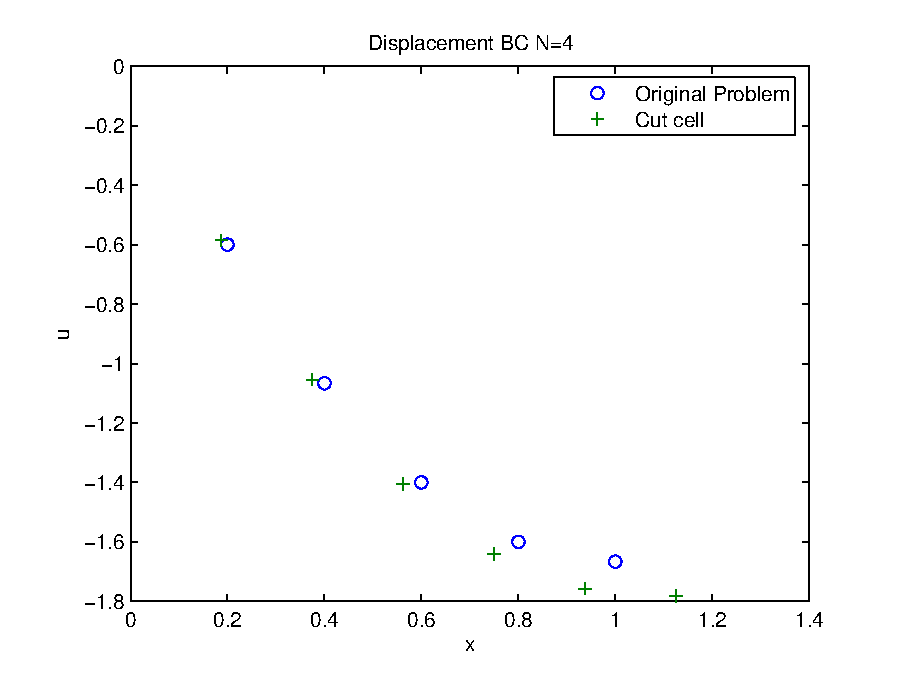
\includegraphics{underintegrationdispbcn4.eps}}
\scalebox{0.5}{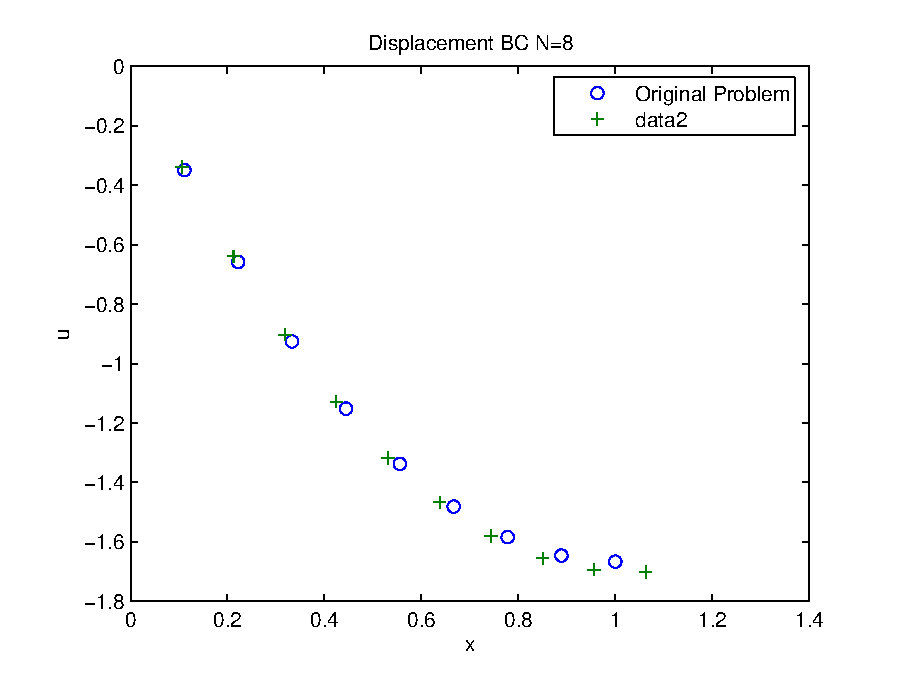
\includegraphics{underintegrationdispbcn8.eps}}\\
\scalebox{0.5}{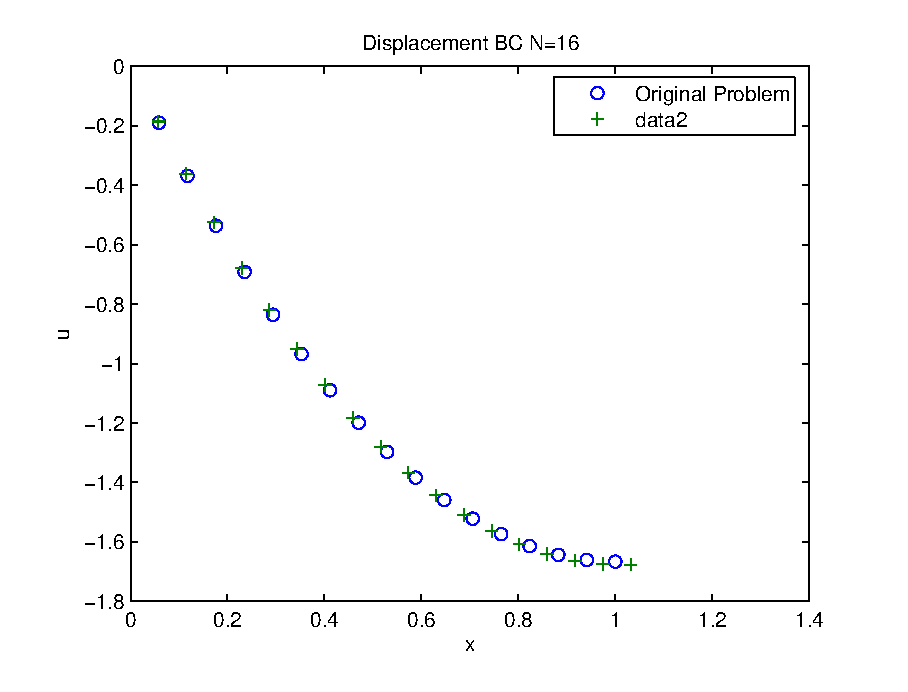
\includegraphics{underintegrationdispbcn16.eps}}
\scalebox{0.5}{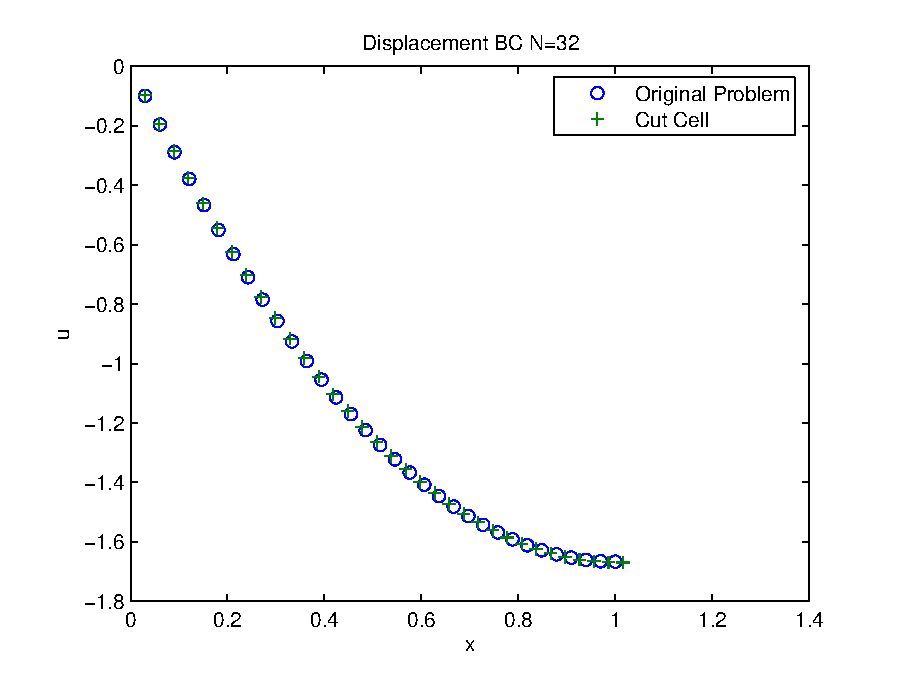
\includegraphics{underintegrationdispbcn32.eps}}\\
\scalebox{0.5}{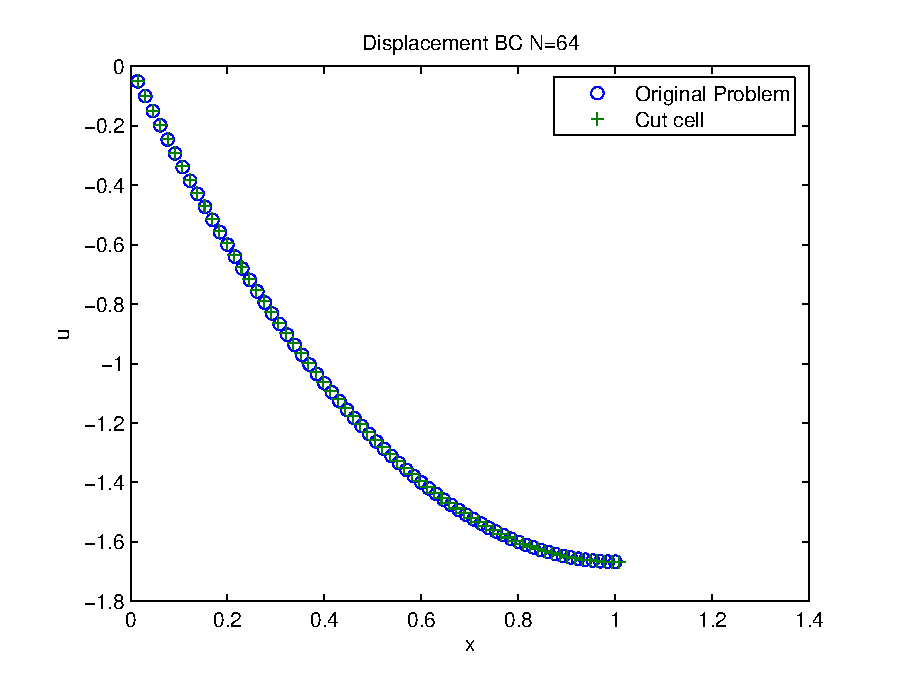
\includegraphics{underintegrationdispbcn64.eps}}\\
\caption{Convergence Study for regular FEM vs. Underintegrated Cut Cell}\label{fig:underintegrationdispbc}
\end{figurehere}
\end{center}
The same problem has been solved, when the actual end of the domain is subject to traction boundary conditions. The other end is still fixed.
\subsection{Second Attempt: Naive Approach}\label{sec:naiveApproach}
Obviously, the problem lies in how to impose the boundary condition, such that it is not associated with an unknown locator (node). A naive idea is to interpolation between some of the nodes, evaluate the intertoplation function at the location of the boundary condition, and obtain a constraint from that, that adds to the total system that needs to be solved.
\subsubsection{Linear Interpolation}
The actual end of the domain lies naturally, due to the choice of the discretization, in the last element. Since we are taking linear elements here, the end of the physical domain lies between two nodes. The solution at the last element is therefore linear, and can be written as (see also figure \ref{fig:linear}):
\begin{eqnarray}
u &=& N_{n-1}(x)u_{n-1}+N_n(x)u_n,\\
N_{n-1}(x) &=& -\frac{(x-\Delta x)}{\Delta x},\\
N_{n}(x) &=& \frac{x}{\Delta x},
\end{eqnarray}
where $u_j$ is the displacement at node $j$ and $\Delta x$ is the size of the element.\\
Imposing the boundary condition, $u\vert_L = \overline{u}$, assuming that the physical domain covers $\alpha \Delta x$ of the element, we obtain the following equation:
\begin{equation}
u = \overline{u} = N_{n-1}(\alpha \Delta x)u_{n-1}+N_n(\alpha \Delta x)u_n.
\end{equation}
\begin{center}
\begin{figurehere} 
\scalebox{0.7}{\input{linearInterpolation.pstex_t}}\\
\caption{Linear Interpolation (constraint on the last element)}\label{fig:linear}
\end{figurehere}
\end{center}
Note here, that the addition of this constraint does not account for a material property of the physical domain in the last element. Note here, that the last element does not get a contribution from the usual finite element setting.\\
In the case, where the body forces $K$ do vanish, the solution is not acceptable. The last element behaves like a foam, satisfies the imposed boundary condition, but does not propagate the information to the neighbor elements about its deformation. The neighbor elements are stiff compared to the last element and do not deform. We thought, that the use of one single element in the interpolation is not enough to forward the information to the entire domain. So, we tried to do the interpolation over the two last elements instead of one.
\subsubsection{Quadratic Interpolation}
The interpolation is done over the two last elements (see figure \ref{fig:quadratic}) and reads now:
\begin{eqnarray}
u &=& N_{n-2}u_{n-2}+N_{n-1}(x)u_{n-1}+N_n(x)u_n,\\
N_{n-2}(x) &=& \frac{(x-\Delta x)(x-2\Delta x)}{2\Delta x^2},\\
N_{n-1}(x) &=& -\frac{x(x-2\Delta x)}{\Delta x^2},\\
N_{n}(x) &=& \frac{x(x-\Delta x)}{2\Delta x^2}.\\
\end{eqnarray}
\begin{center}
\begin{figurehere}
\scalebox{0.7}{\input{quadraticInterpolationf.pstex_t}}\\
\caption{Quadratic Interpolation (constraint on the last two elements)}\label{fig:quadratic}
\end{figurehere}
\end{center}
We noticed the same behavior despite the use of a higher order interpolation. The information is not spread to the neighbor elements, and hence do not deform, due to the large difference in the material properties. 
The results are depicted in figure:
\begin{center}
\begin{figurehere}
\scalebox{0.7}{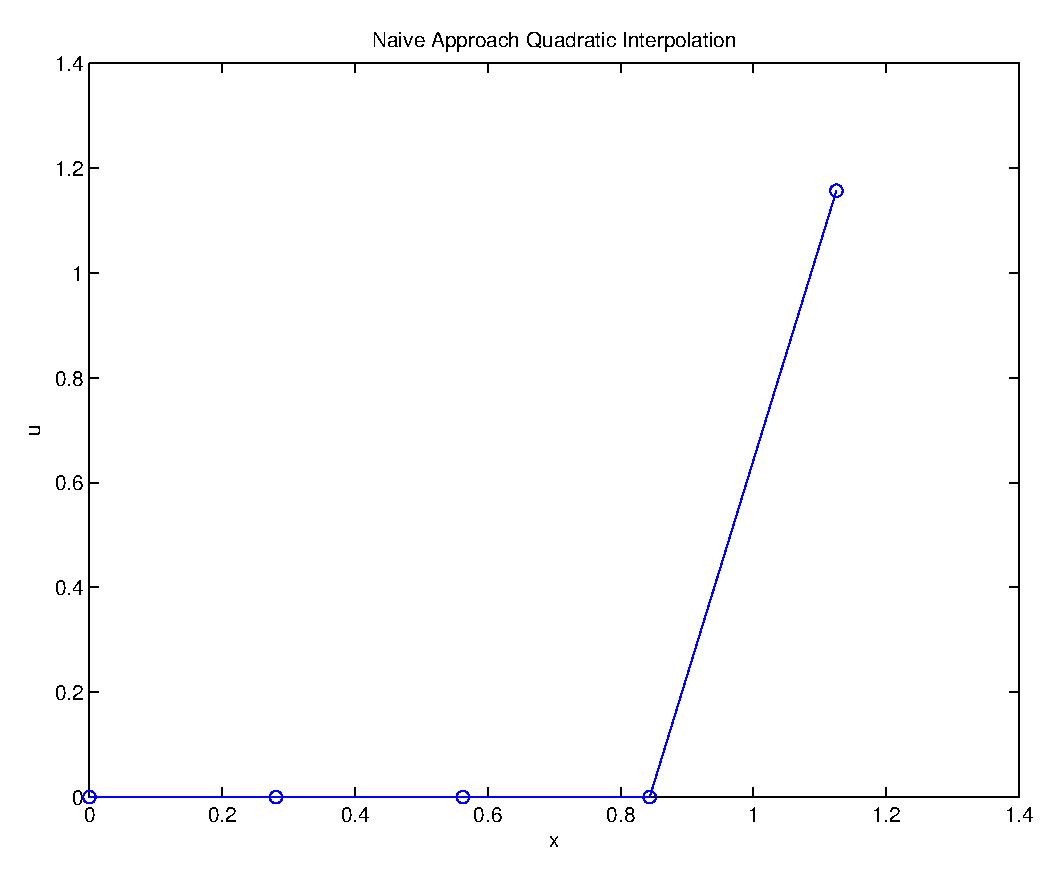
\includegraphics{quadraticResult.eps}}\\
\caption{Result of Quadratic Interpolation}\label{fig:quadraticResult}
\end{figurehere}
\end{center}
\subsubsection{Cubic Interpolation}
The information from three neighbor elements is used to interpolate the value of the displacement boundary condition. 
\begin{eqnarray}
u &=& N_{n-3}u_{n-3}+N_{n-2}u_{n-2}+N_{n-1}(x)u_{n-1}+N_n(x)u_n,\\
N_{n-3}(x) &=& -\frac{(x-\Delta x)(x-2\Delta x)(x-3\Delta x)}{6\Delta x^3}\\
N_{n-2}(x) &=& \frac{x(x-2\Delta x)(x-3\Delta x)}{2\Delta x^3},\\
N_{n-1}(x) &=& -\frac{x(x-\Delta x)(x-3\Delta x)}{2\Delta x^3},\\
N_{n}(x) &=& \frac{x(x-\Delta x)(x-2\Delta x)}{6\Delta x^3}.\\
\end{eqnarray}
\begin{center}
\begin{figurehere} 
\scalebox{0.7}{\input{cubicInterpolation.pstex_t}}\\
\caption{Cubic Interpolation (constraint on the last three elements)}\label{fig:cubic}
\end{figurehere}
\end{center}
The cubic interpolation did not help either, and we obtain the same behavior.
\subsection{Third Attempt: Tranair Approach}
The weak form of the problem given in (\ref{eqn:problem}) reads:
\begin{equation*}
Au_{,x}\xi\vert_0^L - \int Au_{,x}\xi_{,x}\intd x + \int K \xi \intd x= 0,
\end{equation*}
where $\xi$ is the testfunction. 
Since we do not have any traction boundary conditions prescribed, the weak form simplifies to:
\begin{equation*}
- \int Au_{,x}\xi_{,x}\intd x + \int K \xi \intd x= 0.
\end{equation*}
We add the following term, to enforce the Dirichlet boundary conditions:
\begin{equation*}
- \int Au_{,x}\xi_{,x}\intd x + \int K \xi \intd x +  (\xi(u-\overline{u}))\vert_{L}= 0.
\end{equation*}
The stiffness matrix reads:
\begin{equation*}
\mb{K} = - \int Au_{,x}\xi_{,x}\intd x+  (\xi u)\vert_{L}.
\end{equation*}
The force vector reads:
\begin{equation*}
\mb{f} = - \int K \xi \intd x +  \xi\vert_{L}(\overline{u}).
\end{equation*}
Alternatively, we solve using:
\begin{eqnarray*}
\mb{K} =  \int Au_{,x}\xi_{,x}\intd x -  (\xi u)\vert_{L},\\
\mb{f} = \int K \xi \intd x - \xi\vert_{L}(\overline{u}),
\end{eqnarray*}
in order to obtain positive definiteness of the stiffness matrix.
After discretization, the stiffness matrix reads:
\begin{equation*}
\mb{K} = - \int AN_{J,x}N_{I,x}\intd x + (N_I N_J)\vert_{L}.
\end{equation*}
The force vector reads:
\begin{equation*}
\mb{f} = - \int K N_I \intd x +  N_I\vert_{L}(\overline{u}).
\end{equation*}
Consistently considering the signs for positive definiteness, the discretized entries read:
\begin{eqnarray*}
\mb{K} &=&  \int AN_{J,x}N_{I,x}\intd x - (N_I N_J)\vert_{L},\\
\mb{f} &=&  \int K N_I \intd x -  N_I\vert_{L}(\overline{u}).
\end{eqnarray*}
The regular FEM solution to the above problem with a Dirichlet boundary condition $u(x=L) = 0.5$  is depicted in figure \ref{fig:regularFEMSolution}.
\begin{center}
\begin{figurehere} 
\scalebox{0.6}{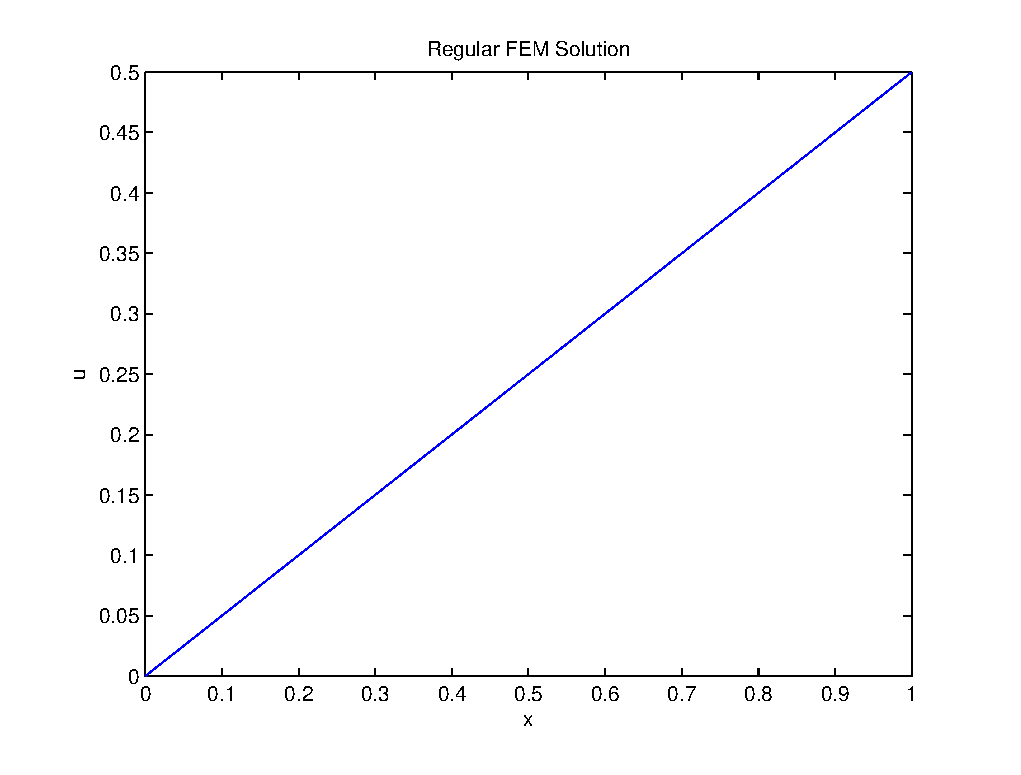
\includegraphics{regularSolutionDisp.eps}}
\caption{Regular FEM Solution}\label{fig:regularFEMSolution}
\end{figurehere}
\end{center}
\subsubsection{With consideration of the DE contribution to the entire element}
For the cut cell element, only the differential equation resolved over the part of the element that does belong to the physical domain is considered. Hence the multiplication with the ratio of the physical domain to the total element length $\alpha$.
If we consider the differential equation contribution to the last element, and we weight the contributions to the stiffness and the load vector with a penalty parameter $P^*$, i.e.
\begin{equation*}
\mb{K} = - \alpha \int AN_{J,x}N_{I,x}\intd x + P^*(N_I N_J)\vert_{L},
\end{equation*}
and
\begin{equation*}
\mb{f} = - \alpha \int K N_I \intd x +  P^*N_I\vert_{L}(\overline{u}),
\end{equation*}
and if we consistently consider the signs for positive definiteness
\begin{eqnarray*}
\mb{K} &=&  \alpha \int AN_{J,x}N_{I,x}\intd x - P^*(N_I N_J)\vert_{L},\\
\mb{f} &=&  \alpha \int K N_I \intd x -  P^*N_I\vert_{L}(\overline{u}),
\end{eqnarray*}
we obtain the results presented in \ref{fig:withcontDE}:
\begin{center}
\begin{figurehere}
\scalebox{0.4}{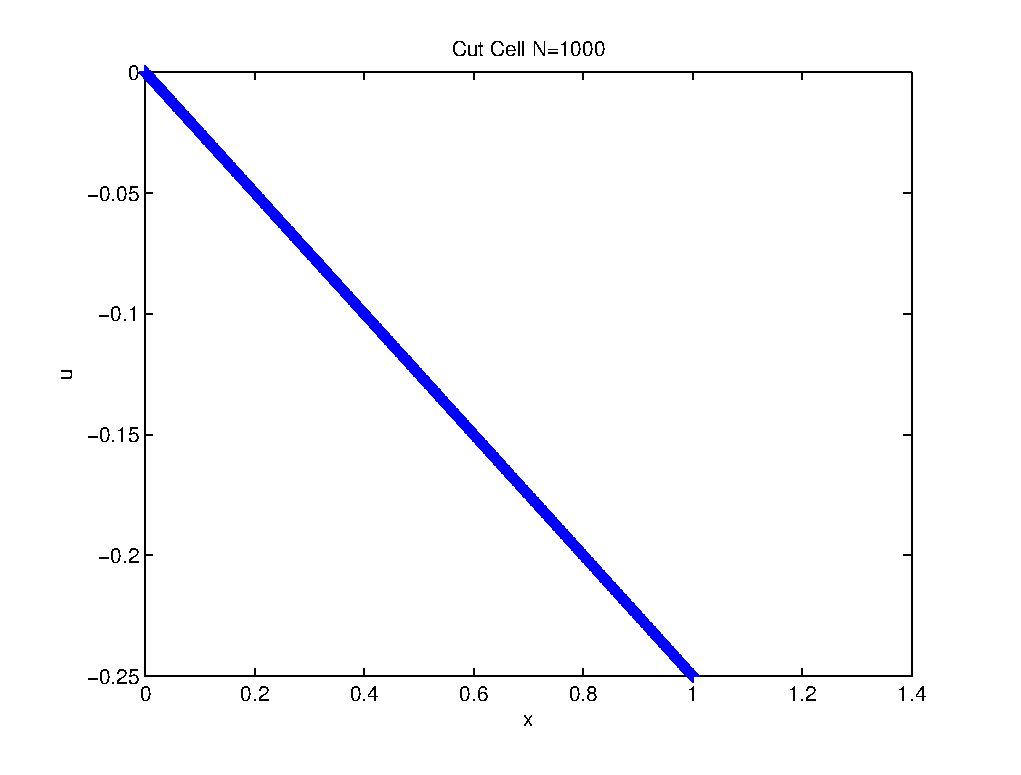
\includegraphics{cutCellPenalty1.eps}}
\scalebox{0.4}{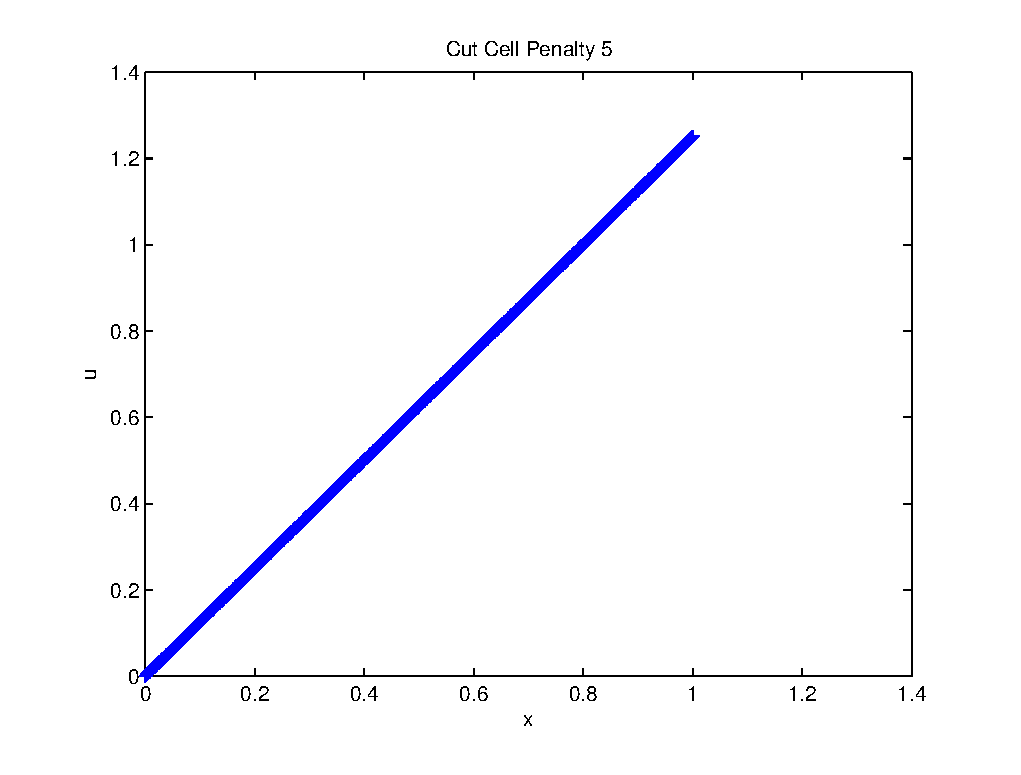
\includegraphics{cutCellPenalty5.eps}}\\
\scalebox{0.4}{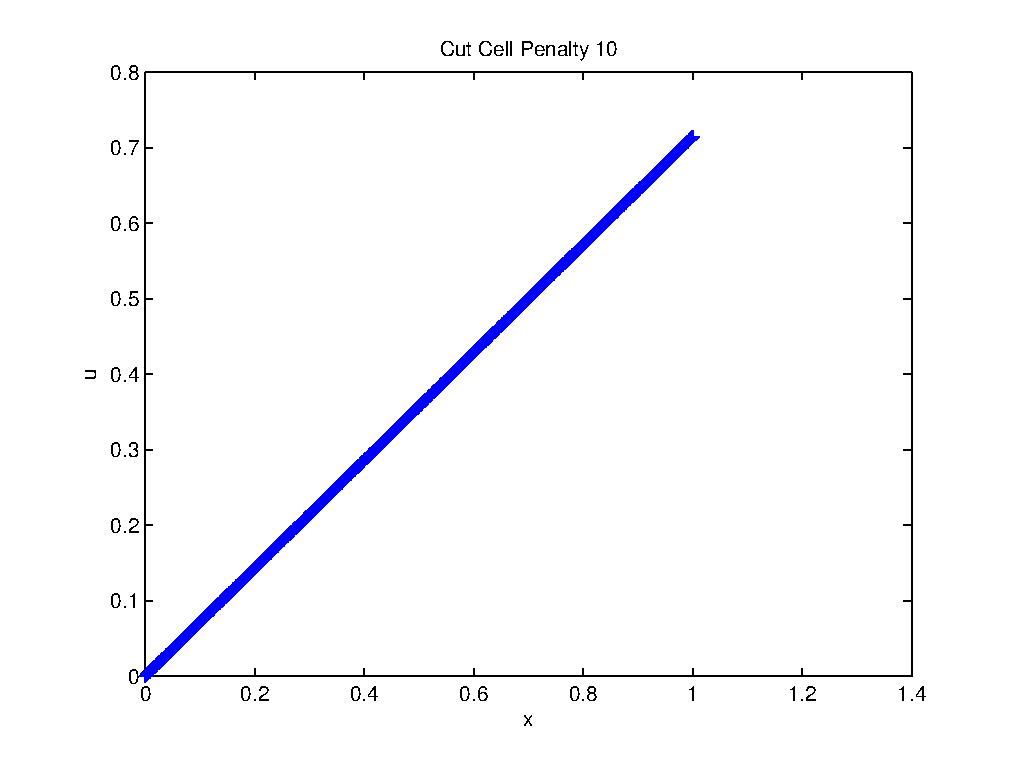
\includegraphics{cutCellPenalty10.eps}}
\scalebox{0.4}{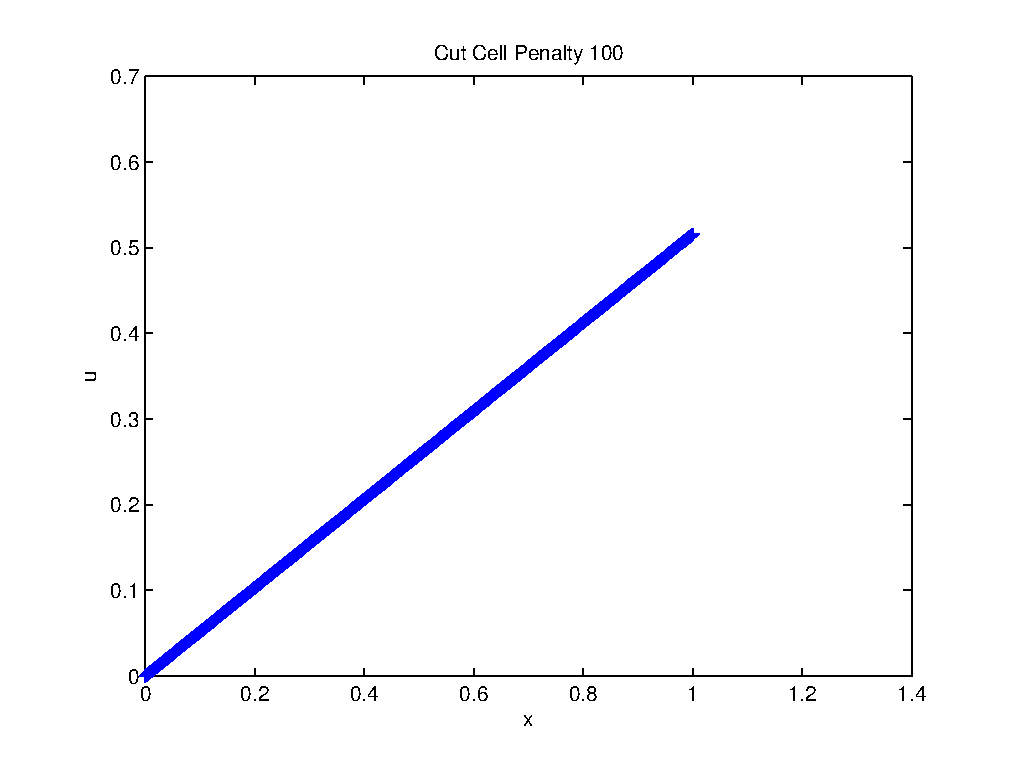
\includegraphics{cutCellPenalty100.eps}}\\
\scalebox{0.4}{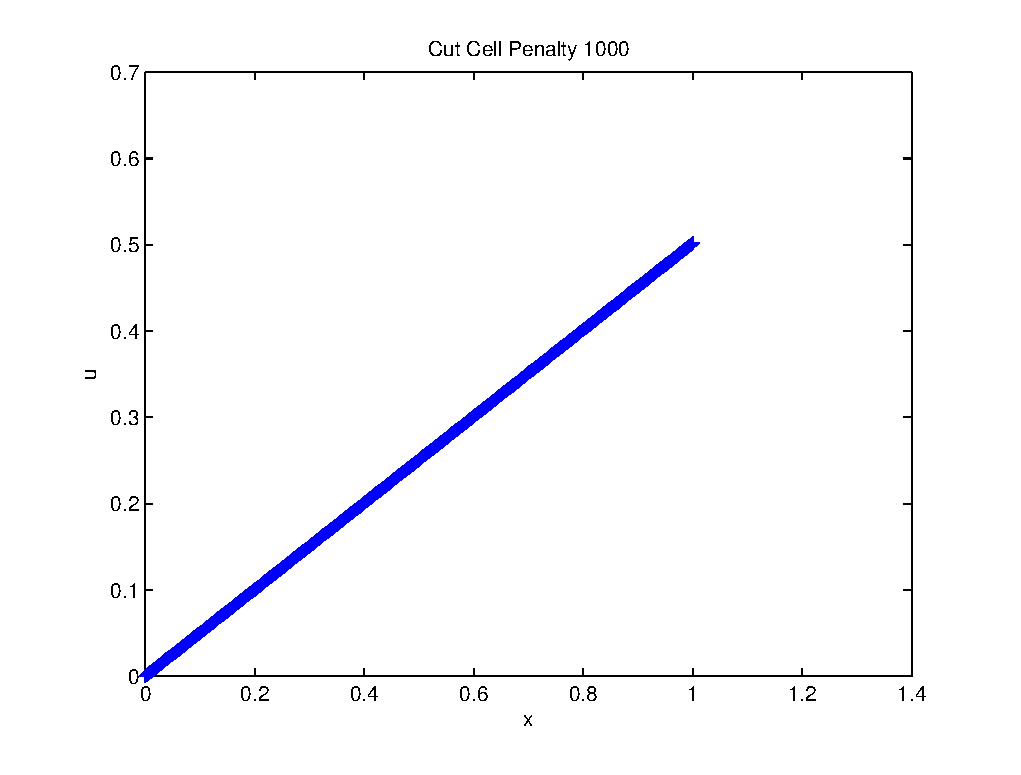
\includegraphics{cutCellPenalty1000.eps}}
\caption{Cut Cell Solution for different weight factors $1$ ,$5$ ,$10$, $100$ and $1000$}\label{fig:withcontDE}
\end{figurehere}
\end{center}
The summary of the effect of the weight parameter on the deflection of the end tip of the one-dimensional domain is given in figure \ref{fig:summaryPenalty}:
\begin{center}
\begin{figurehere} 
\scalebox{0.6}{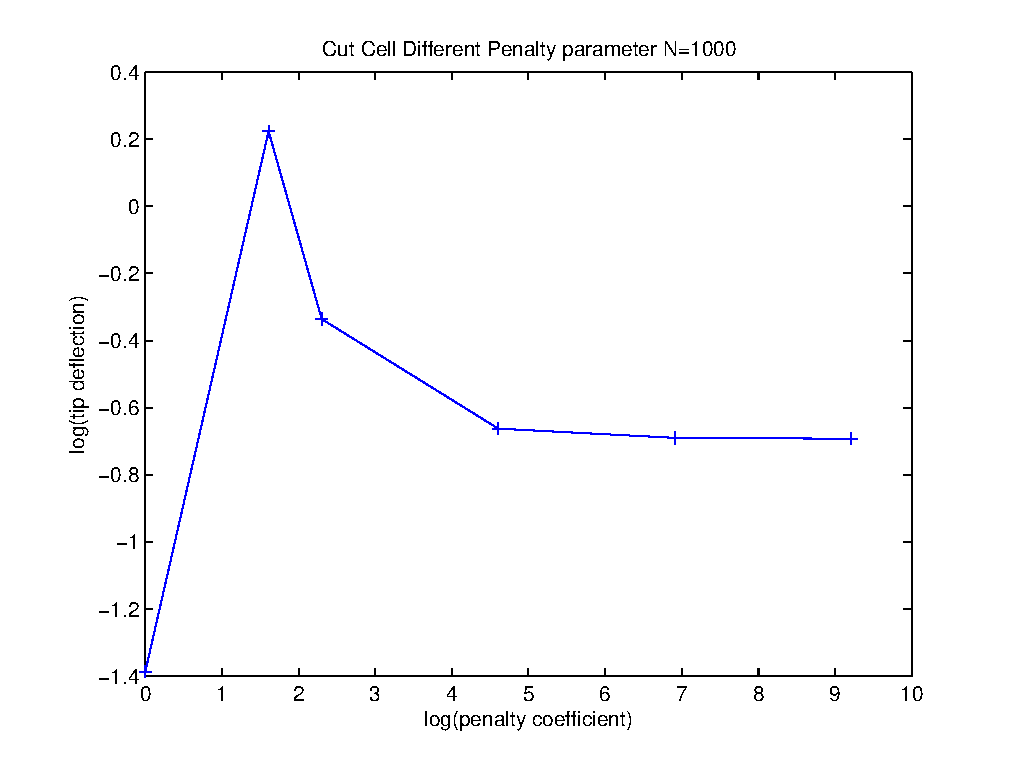
\includegraphics{summarypenalty.eps}}
\caption{Effect of weight factor on the solution}\label{fig:summaryPenalty}
\end{figurehere}
\end{center}
\begin{center}
\begin{figurehere} 
\scalebox{0.6}{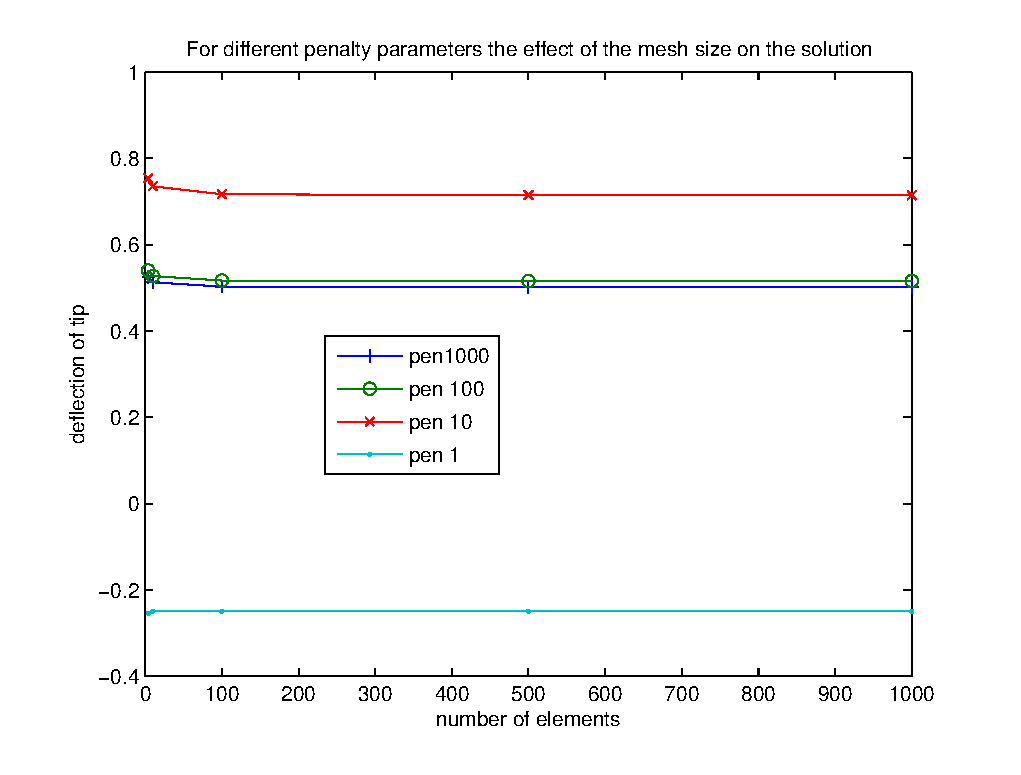
\includegraphics{effectMeshSizePen.eps}}
\caption{Effect of mesh size on the solution for different weight factors}\label{fig:summaryPenaltyMeshSize}
\end{figurehere}
\end{center}
\subsubsection{Without consideration of the DE contribution to the element}
If we do not consider the contributions from the differential equation to the last element, i.e.
\begin{equation*}
\mb{K} =  P^*(N_I N_J)\vert_{L},
\end{equation*}
and
\begin{equation*}
\mb{f} = P^*N_I\vert_{L}(\overline{u}),
\end{equation*}
we return to the naive approach we tried before (section \ref{sec:naiveApproach}).
The results are depicted in figure \ref{fig:withoutcont}.
\begin{center}
\begin{figurehere} 
\scalebox{0.6}{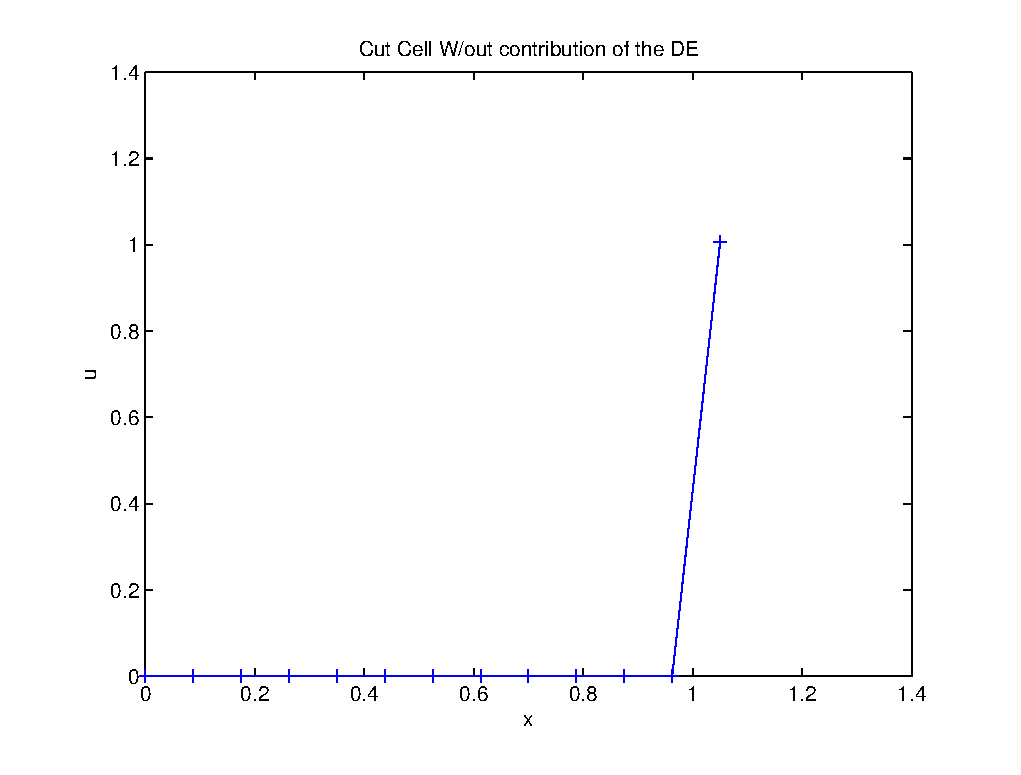
\includegraphics{cutCellwithoutcontrDE.eps}}
\scalebox{0.6}{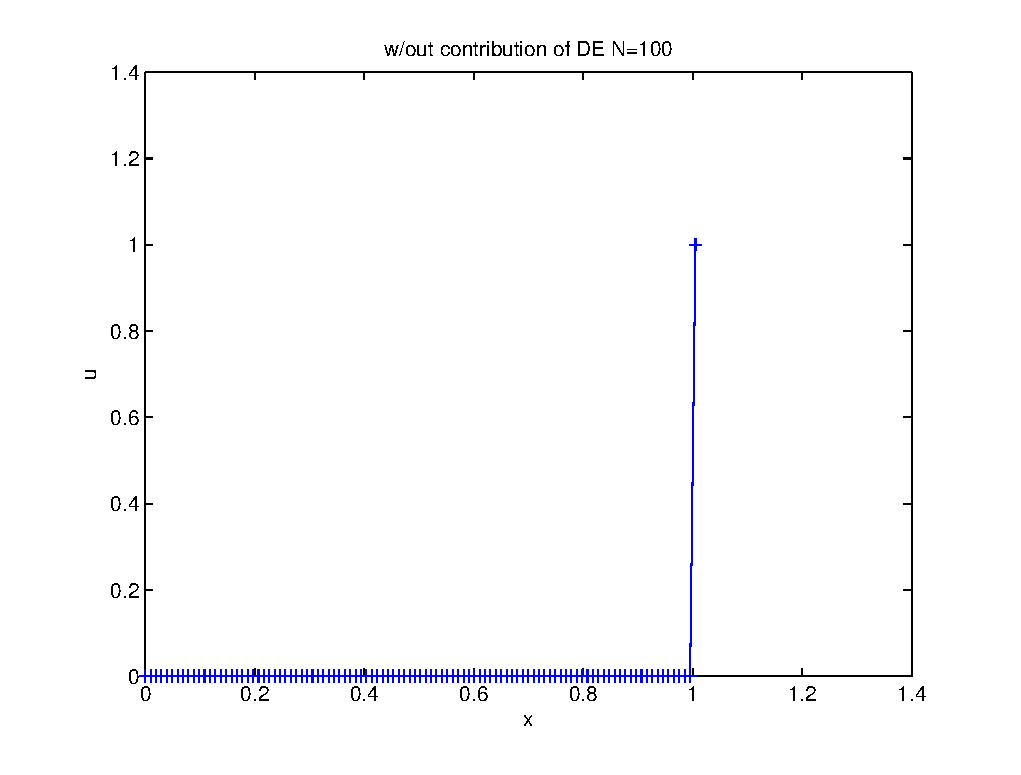
\includegraphics{cutCellwithoutcontrDE100.eps}}\\
\caption{Without considering the contribution of the DE to the last element}\label{fig:withoutcont}
\end{figurehere}
\end{center}

\subsection{Finite Volume Method (Prof. Papadopoulos Approach)}\label{sec:PPfinitevolume}
As the above described attempts have failed, we wanted to understand the treatment of the cut cells in the finite volume method, and
map the similarities to the finite element method, to figure out the correct method.\footnote{This approach has been derived by Prof. Papadopolous. According to Prof. Colella, this approach corresponds to the Shortley-Weller scheme, published in 1938.}
\subsubsection{One dimensional finite volume method}
We want to solve the same problem given in (\ref{eqn:problem}). Th system is discretized into $n$ control volumes [$x_i$, $x_{i+1}$]. Each control volume is assigned a centroid $x_{i+\frac{1}{2}}$ defined by:
\begin{equation}
x_{i+\frac{1}{2}} = \frac{x_i + x_{i+1}}{2}.
\end{equation}
See Figure \ref{fig:domain}.
\begin{center}
\begin{figurehere}
\input{domain.pstex_t}
\caption{Domain discretization}\label{fig:domain}
\end{figurehere}
\end{center}
We consider Dirichlet boundary conditions on both ends:
\begin{eqnarray}
u(0) &=& \overline{u}_0,\\
u(L) &=& \overline{u}_L.
\end{eqnarray}
The problem can be considered in every cell, s.t.
\begin{eqnarray}
Au_{,xx} &=& \frac{1}{\Delta x}\int_{x_i}^{x_{i+1}}Au_{,xx}\intd x,\\
\Delta x &=& x_{i+1} - x_{i}.
\end{eqnarray}
Using the mid-point rule, the above expression can be approximated by:
\begin{eqnarray}
Au_{,xx} &=& \frac{1}{\Delta x}\Delta x Au_{,xx}\vert_{x_{i+\frac{1}{2}}},\\
&\simeq& Au_{,xx}\vert_{x_{i+\frac{1}{2}}}.
\end{eqnarray}
Hence, the problem is solved locally in each volume element:
\begin{eqnarray}
Au_{,xx}\vert_{x_{i+\frac{1}{2}}} = -K.
\end{eqnarray}
The second order derivative at the centroids is approximated using a Taylor series expansion, assuming that the remainder term vanishes as the control volume size becomes smaller and smaller. We have:
\begin{eqnarray}
u(x_{i+\frac{3}{2}}) = u(x_{i + \frac{1}{2}}) + u_{,x}\vert_{x_{i+\frac{1}{2}}} + \frac{\Delta x^2}{2}u_{,xx}\vert_{x_{i+\frac{1}{2}}}+\frac{\Delta x^3}{6}u_{,xxx}\vert_{x_{i+\frac{1}{2}}}+\frac{\Delta x^4}{24}u_{,xxxx}\vert_{x_i+\xi_1\Delta x},\\
u(x_{i-\frac{1}{2}}) = u(x_{i + \frac{1}{2}}) - u_{,x}\vert_{x_{i+\frac{1}{2}}} + \frac{\Delta x^2}{2}u_{,xx}\vert_{x_{i+\frac{1}{2}}}-\frac{\Delta x^3}{6}u_{,xxx}\vert_{x_{i+\frac{1}{2}}}+\frac{\Delta x^4}{24}u_{,xxxx}\vert_{x_i+\xi_2\Delta x}.
\end{eqnarray}
Adding these last equations, we obtain:
\begin{eqnarray}
u_{,xx}\vert{x_{i+\frac{1}{2}}} = \frac{u(x_{i+\frac{3}{2}})+u(x_{i-\frac{1}{2}})-2u(x_{i+\frac{1}{2}})}{\Delta x^2},
\end{eqnarray}
with
\begin{eqnarray}
\frac{\Delta x^4}{24}u_{,xxxx}\vert_{x_i+\xi_1\Delta x}\rightarrow 0,\\
\frac{\Delta x^4}{24}u_{,xxxx}\vert_{x_i+\xi_2\Delta x}\rightarrow 0.
\end{eqnarray}
We obtain equations for the centroids of the inner volumes:
\begin{eqnarray}
A\frac{u(x_{i+\frac{3}{2}})+u(x_{i-\frac{1}{2}})-2u(x_{i+\frac{1}{2}})}{\Delta x^2}&=&-K,\\
u(x_{i+\frac{3}{2}})+u(x_{i-\frac{1}{2}})-2u(x_{i+\frac{1}{2}}) &=& \frac{-K\Delta x^2}{A}.
\end{eqnarray}
Clearly, this is not the case for the boundary volume elements. The way we proceed is to build a ghost centroid adjacent to the centroid we are looking at, as depicted in figure \ref{fig:ghostcentroid}.
\begin{center}
\begin{figurehere} 
\input{ghostcentroid.pstex_t}
\caption{Ghost centroid}\label{fig:ghostcentroid}
\end{figurehere}
\end{center}

However, we do not want to introduce new unknowns through the ghost centroids. The solution at the ghost centroids is defined by the Dirichlet boundary conditions.
The equation on the left boundary volume centroid reads:
\begin{eqnarray}
u(\Delta x) &=& N_1(\Delta x)u_g + N_2(\Delta x)u_{\frac{1}{2}} + N_3u_{\frac{3}{2}},\\
&=& \overline{u}_0,\\
N_1(x) &=& \frac{(x-\frac{3\Delta x}{2})(x - \frac{5\Delta x}{2})}{2\Delta x^2},\\
N_1(\Delta x) &=& \frac{3}{8},\\
N_2(x) &=& -\frac{(x-\frac{\Delta x}{2})(x - \frac{5\Delta x}{2})}{\Delta x^2},\\
N_2(\Delta x) &=& \frac{3}{4},\\
N_3(x) &=& \frac{(x-\frac{\Delta x}{2})(x - \frac{3\Delta x}{2})}{2\Delta x^2},\\
N_3(\Delta x) &=& -\frac{1}{8}.
\end{eqnarray}
At the end, we obtain:
\begin{eqnarray}
u_g &=& \frac{8}{3}(\overline{u}_0 -\frac{3}{4}u_{\frac{1}{2}} + \frac{1}{8} u_{\frac{3}{2}}),\\
-4 u_{\frac{1}{2}} + \frac{4}{3}u_{\frac{3}{2}} &=& \frac{-K\Delta x^2}{A} - \frac{8}{3}\overline{u}_0.
\end{eqnarray}
Analogously, we obtain an equation for the right boundary volume centroid:
\begin{eqnarray}
u_{gL} &=& \frac{8}{3}(\overline{u}_L -\frac{3}{4}u_{n-\frac{3}{2}} + \frac{1}{8} u_{n-\frac{1}{2}}),\\
-4 u_{n-\frac{1}{2}} + \frac{4}{3}u_{n-\frac{3}{2}} &=& \frac{-K\Delta x^2}{A} - \frac{8}{3}\overline{u}_L,
\end{eqnarray}
with $n$ the total number of vertices.
Finally, the system of equations reads:
\begin{eqnarray}
-4 u_{\frac{1}{2}} + \frac{4}{3}u_{\frac{3}{2}} &=& \frac{-K\Delta x^2}{A} - \frac{8}{3}\overline{u}_0,\\
u(x_{i+\frac{3}{2}})+u(x_{i-\frac{1}{2}})-2u(x_{i+\frac{1}{2}}) &=& \frac{-K\Delta x^2}{A},\hspace*{0.5cm} i=1,n-2\\
-4 u_{n-\frac{1}{2}} + \frac{4}{3}u_{n-\frac{3}{2}} &=& \frac{-K\Delta x^2}{A} - \frac{8}{3}\overline{u}_L.
\end{eqnarray}
\subsubsection{Results}
The system has been solved with $A=3$, $K=0$, $L=1$. $\overline{u}_0 = 0$ and $\overline{u}_L=0.5$.
The solution is depicted in figure:
\begin{center}
\begin{figurehere} 
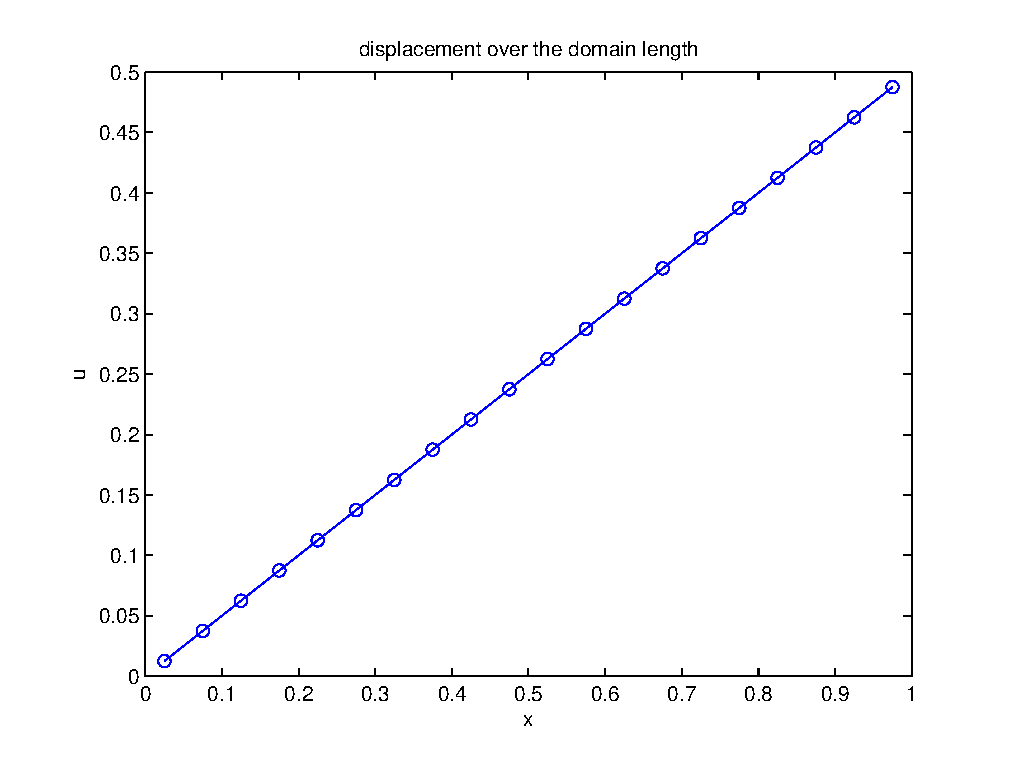
\includegraphics{finitevol1d.eps}
\caption{Solution}\label{fig:finitevol}
\end{figurehere}
\end{center}
\subsubsection{Cut Cell}
In the case where the last control volume is not fully covered by the physical domain, the expressions for last system equation changes depending on the length ratio of the physical domain with respect to the full cell $\alpha$. The above given expressions correspond to the special case, where $\alpha = 1$.
The equation for the right boundary volume centroid reads now with:
\begin{eqnarray}
u_{gL} = \frac{1}{N_3}(\overline{u}_L -N_1\Delta x)u_{n-\frac{3}{2}} -N2\Delta x) u_{n-\frac{1}{2}}),\\
-(2+\frac{N_2}{N_3}) u_{n-\frac{1}{2}} + (1-\frac{N_2}{N_3})u_{n-\frac{3}{2}} = \frac{-K\Delta x^2}{A} - \frac{1}{N_3}\overline{u}_L,\\
N_1 = N_1((1+\alpha)\Delta x),\\
N_2 = N_2((1+\alpha)\Delta x),\\
N_3 = N_3((1+\alpha)\Delta x).
\end{eqnarray}
The total system of equation reads:
\begin{eqnarray}
-4 u_{\frac{1}{2}} + \frac{4}{3}u_{\frac{3}{2}} &=& \frac{-K\Delta x^2}{A} - \frac{8}{3}\overline{u}_0,\\
u(x_{i+\frac{3}{2}})+u(x_{i-\frac{1}{2}})-2u(x_{i+\frac{1}{2}}) &=& \frac{-K\Delta x^2}{A},\hspace*{0.5cm} i=1,n-2\\
-(2+\frac{N_2}{N_3}) u_{n-\frac{1}{2}} + (1-\frac{N_2}{N_3})u_{n-\frac{3}{2}} &=& \frac{-K\Delta x^2}{A} - \frac{1}{N_3}\overline{u}_L.
\end{eqnarray}
For different values of $\alpha$, the system has been solved and the solutions are depicted in figure \ref{fig:finitevolcutPP}:
\begin{center}
\begin{figurehere}
\scalebox{0.35}{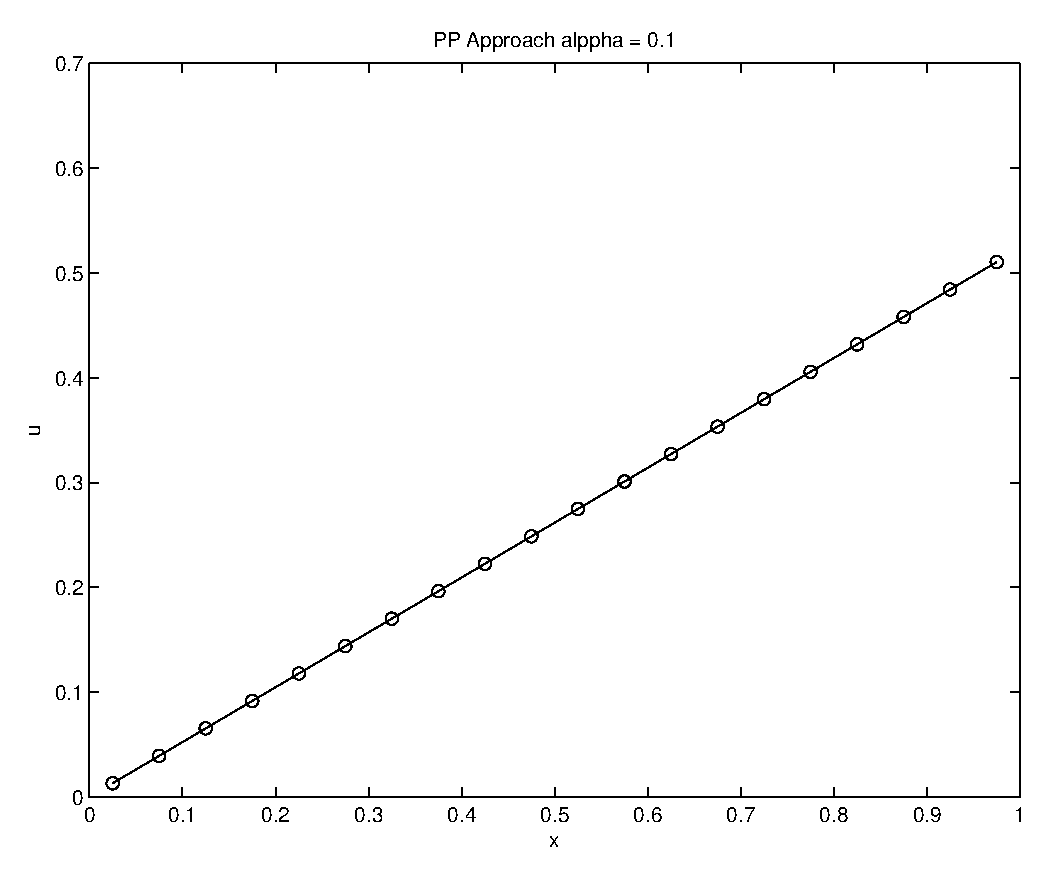
\includegraphics{alpha01.eps}}
\scalebox{0.35}{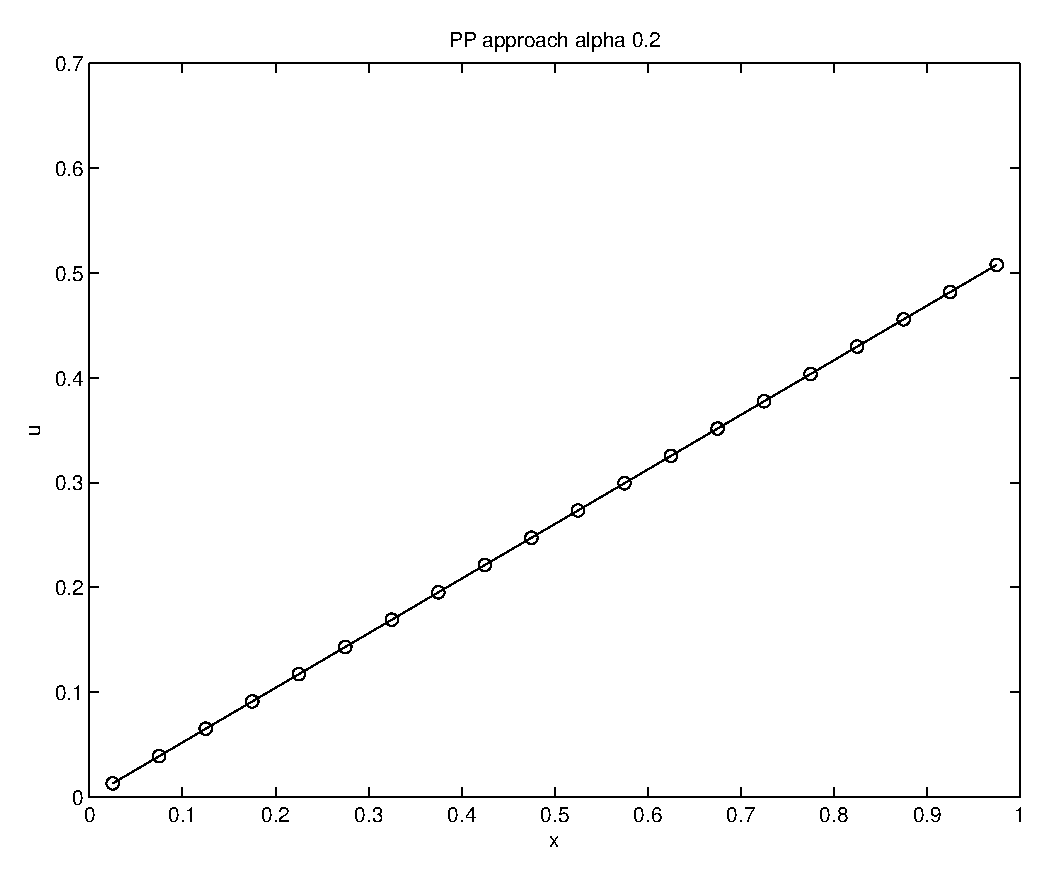
\includegraphics{alpha02.eps}}\\
\scalebox{0.35}{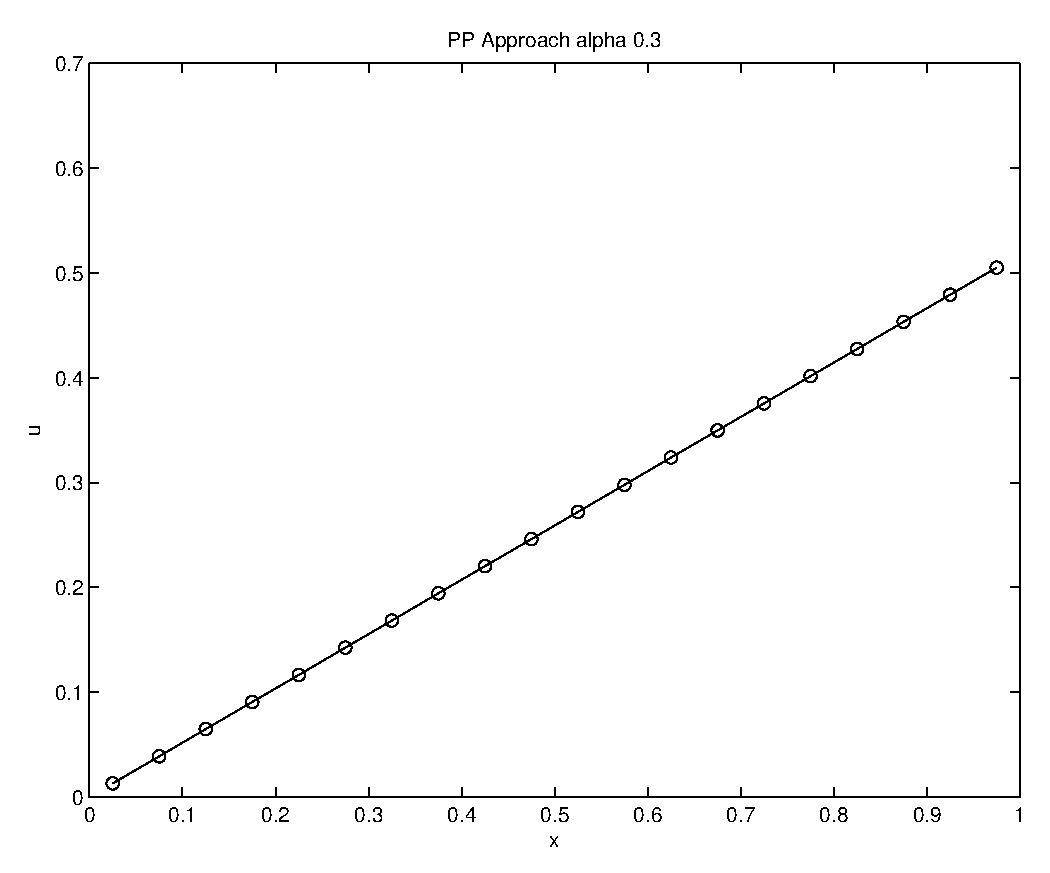
\includegraphics{alpha03.eps}}
\scalebox{0.35}{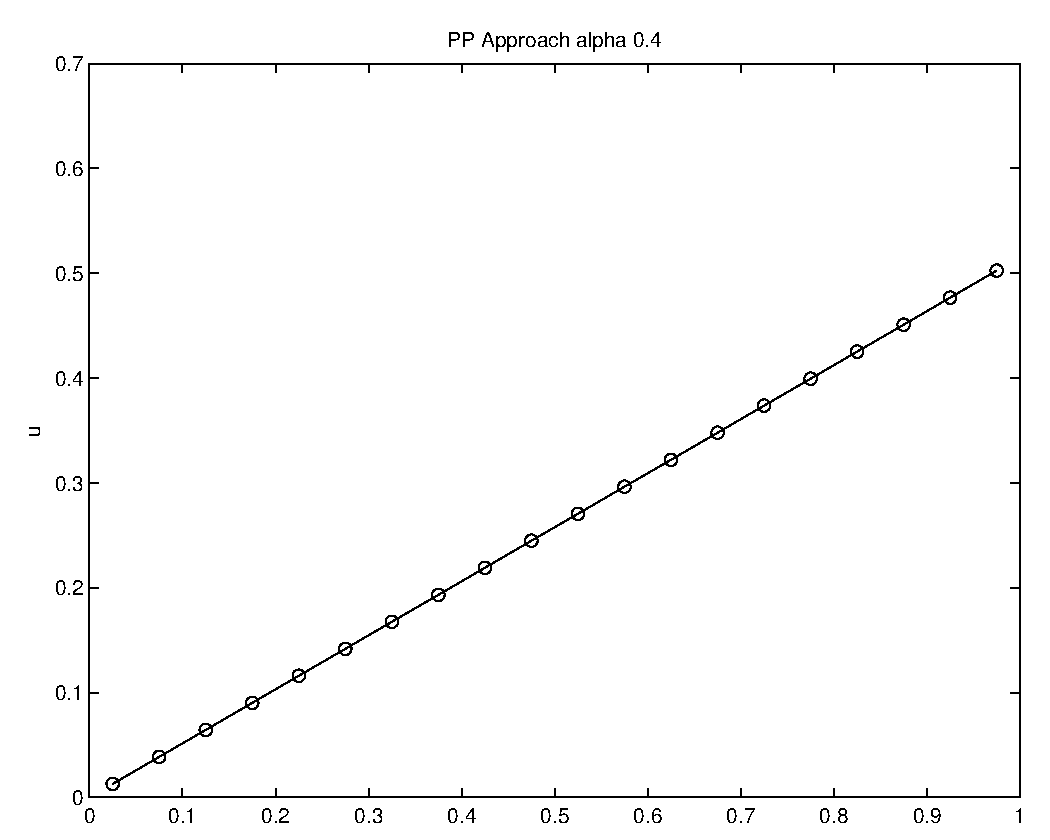
\includegraphics{alpha04.eps}}\\
\scalebox{0.35}{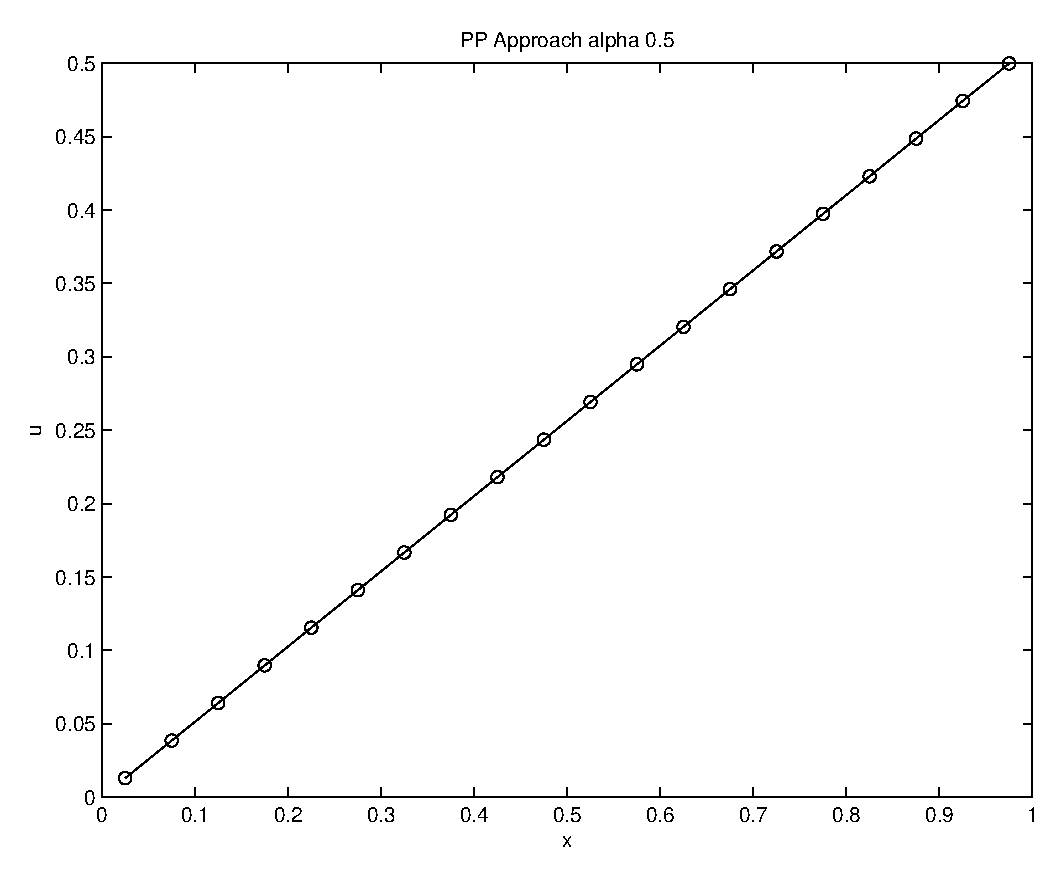
\includegraphics{alpha05.eps}}
\scalebox{0.35}{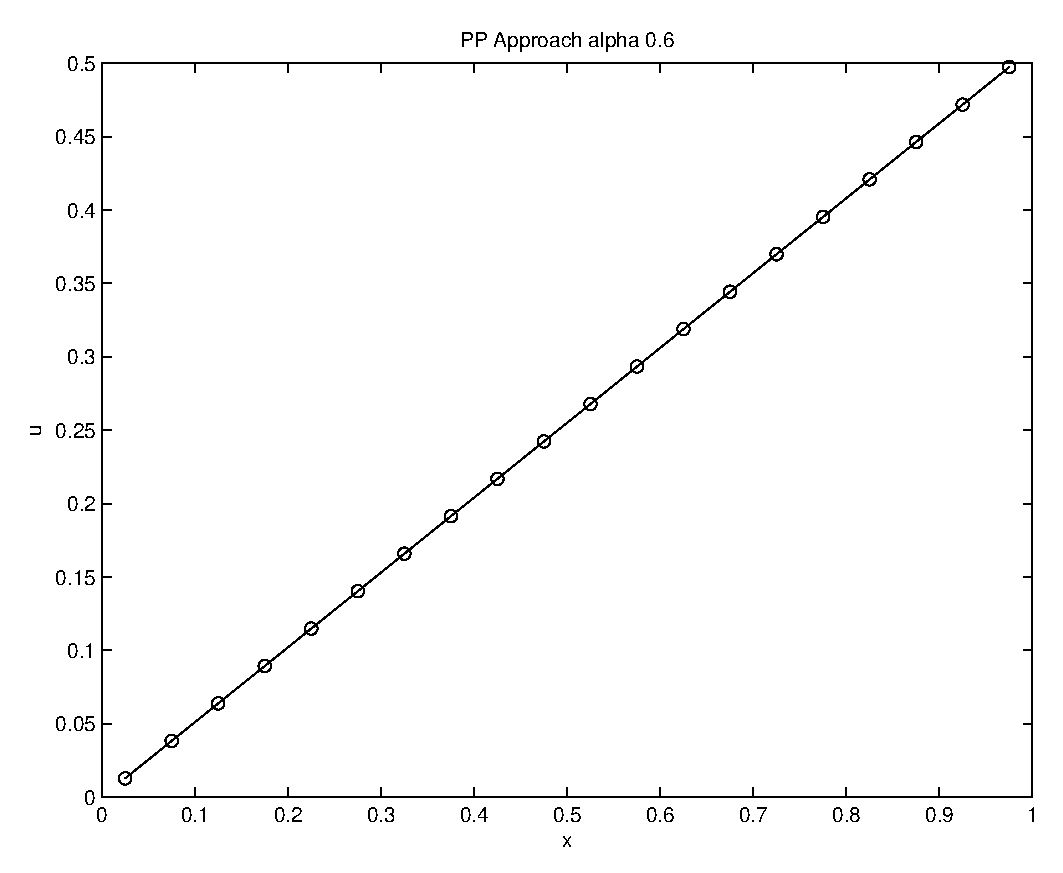
\includegraphics{alpha06.eps}}\\
\scalebox{0.35}{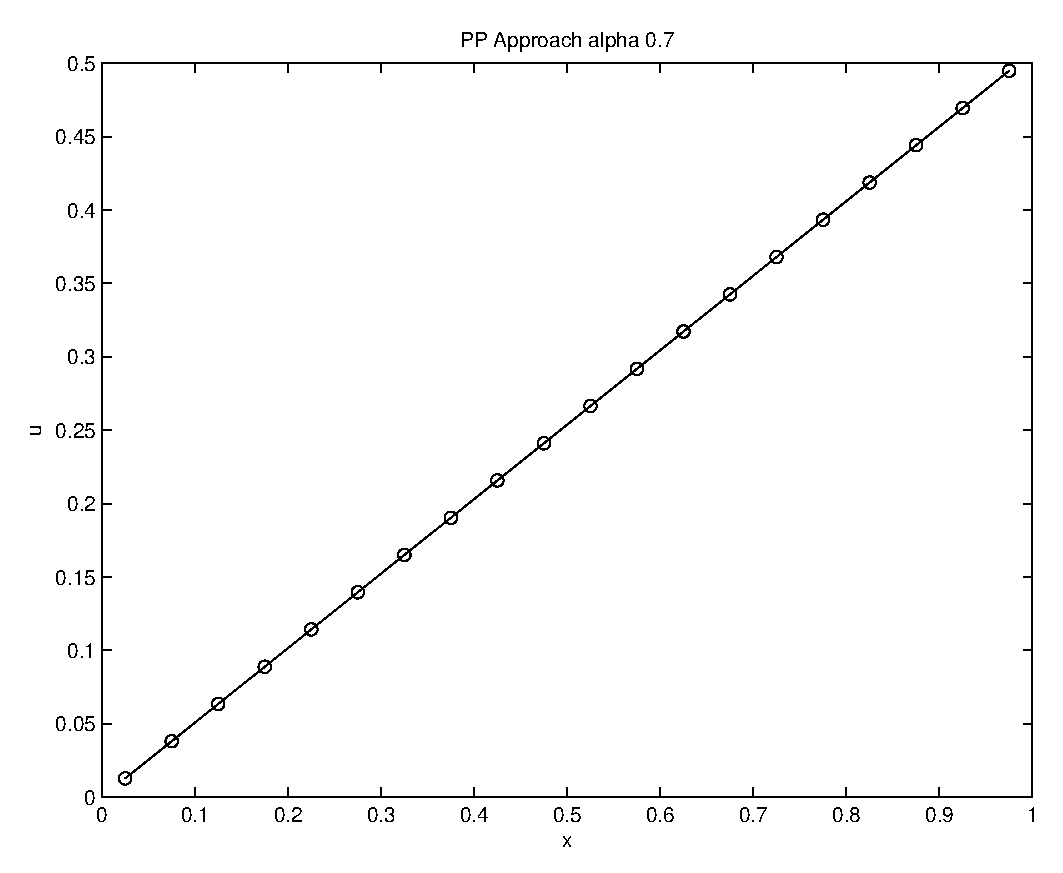
\includegraphics{alpha07.eps}}
\scalebox{0.35}{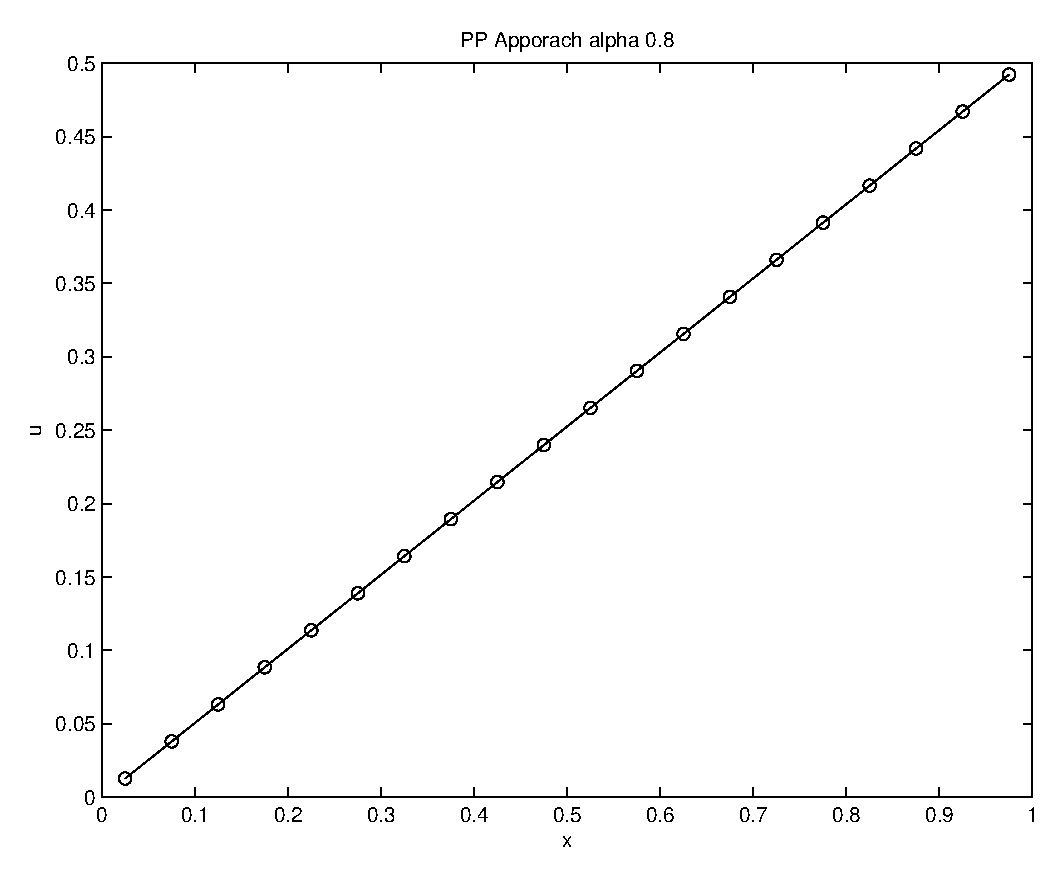
\includegraphics{alpha08.eps}}\\
\caption{Solution With Cut Cell for different values of $\alpha$}\label{fig:finitevolcutPP}
\end{figurehere}
\end{center}
\subsection{First Attempt: Finite Volume Method (Prof. Colella Approach)}
\subsubsection{Theory}
The same problem stated in (\ref{eqn:problem}) is going to be solved here. We obtain an equation at each centroid of a cell.
\begin{eqnarray}
\frac{\partial ^2 u}{\partial x^2}\vert_{x_{i+\frac{1}{2}}}  &=& \frac{-K}{A},\\
\Leftrightarrow \frac{1}{\Delta x}(\frac{\partial u}{\partial x}\vert_{R} -\frac{\partial u}{\partial x}\vert_{L}) &=& \frac{-K}{A},
\end{eqnarray}
where $R$ is the next vertex to the right and $L$ to the next vertex to the left.\\
At an inner element, the approximation of the second derivative reads:
\begin{eqnarray}
\Leftrightarrow \frac{1}{\Delta x}(\frac{\partial u}{\partial x}\vert_{R} -\frac{\partial u}{\partial x}\vert_{L}) &=& \frac{1}{\Delta x}(\frac{1}{\Delta x}(u_{i+2}-u_{i}) - \frac{1}{\Delta x}(u_{i+1}-u_{i-1})),\\
&=& \frac{1}{\Delta x^2}(u_{i+2}-u_{i}-u_{i+1}+u_{i-1}),
\end{eqnarray}
where $u_{i-1}$, $u_{i}$, $u_{i+1}$ and $u_{i+2}$ are the nodal (vertices) displacements. \footnote{This was a major misunderstanding in the theory of finite volumes. The equations are written at the centroids, as well as the unknowns are held at the centroids and not at the node as done above. The wrong way to do it leads to an issue if the last element is a full. In this case we have more equations than unknowns, assuming that boundary conditions are prescribed on both ends. If one of the unknowns is  a free end and we have a cut cell, we have less equations than unknowns. This is very obvious sign that there is a misunderstanding. The theory is not going to be derived based on this wrong assumption. The correct theory is going to be derived in section \ref{sec:PCCutCellTheory} }
\subsubsection{Results}
The system has been solved with $A=3$, $K=0$, $L=1$. $\overline{u}_0 = 0$ and $\overline{u}_L=0.5$.\footnote{There is a mistake in the understanding of the theory. That is the explanation for the oscillatory behavior of the solution, that is not compatible with the properties of the solution to an elliptic equation. A solution to an elliptic equation is necessarily not oscillatory.}
\begin{center}
\begin{figurehere}
\scalebox{0.45}{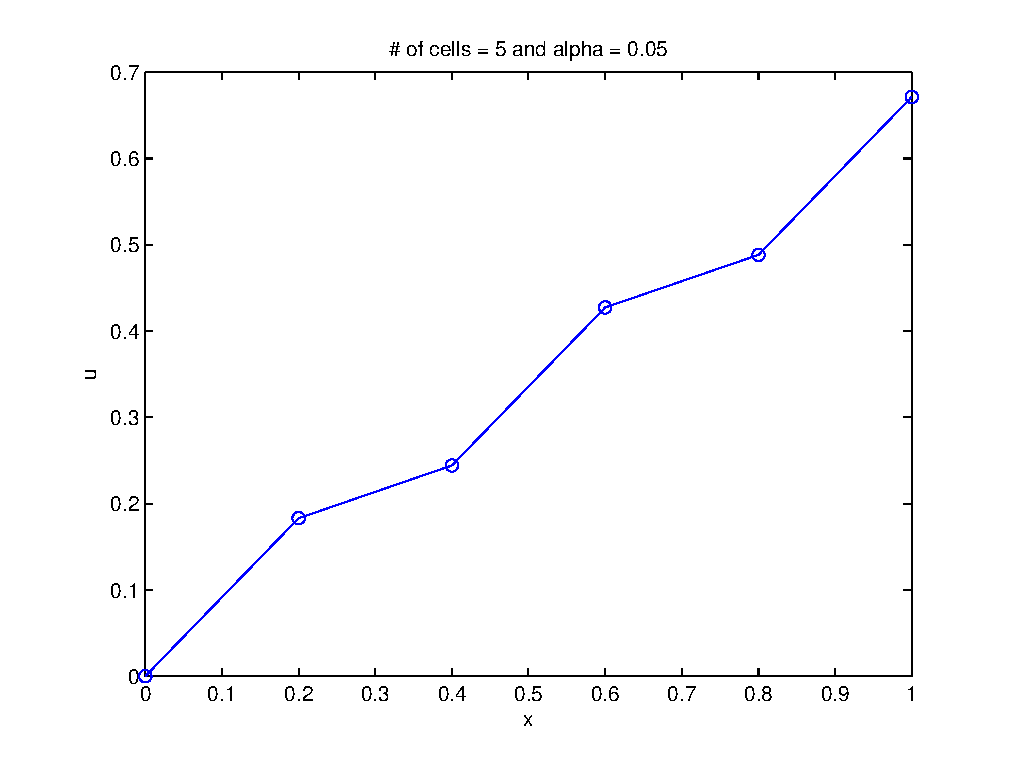
\includegraphics{conv5alpha005.eps}}
\scalebox{0.45}{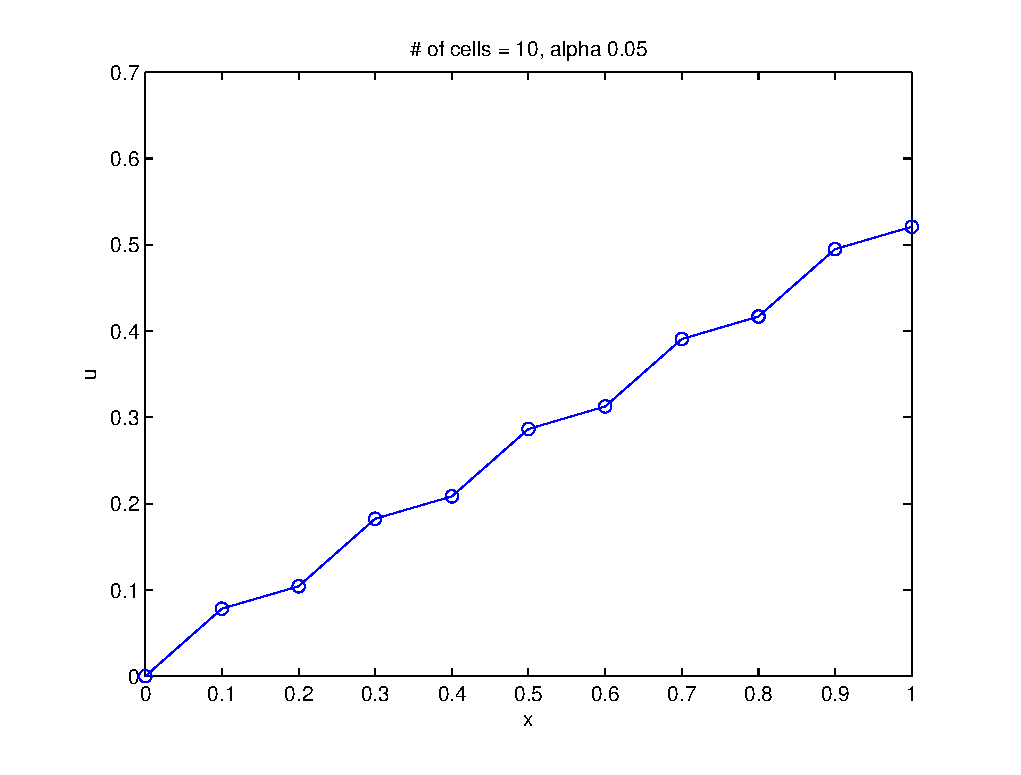
\includegraphics{conv10alpha005.eps}}
\scalebox{0.45}{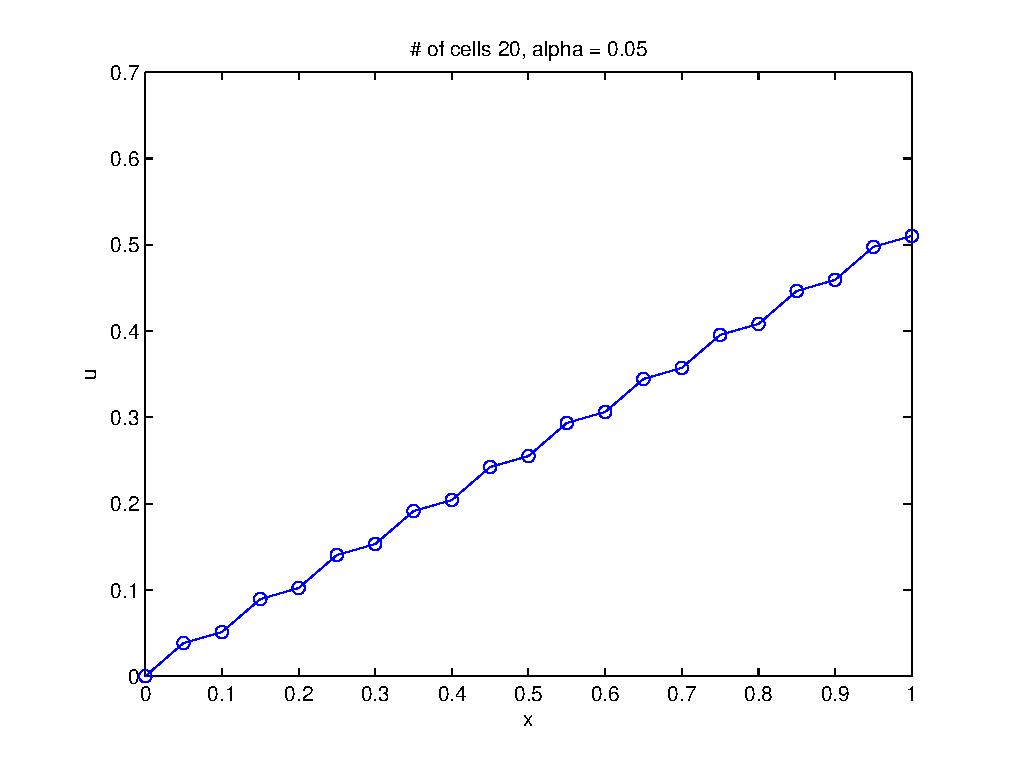
\includegraphics{conv20alpha005.eps}}
\scalebox{0.45}{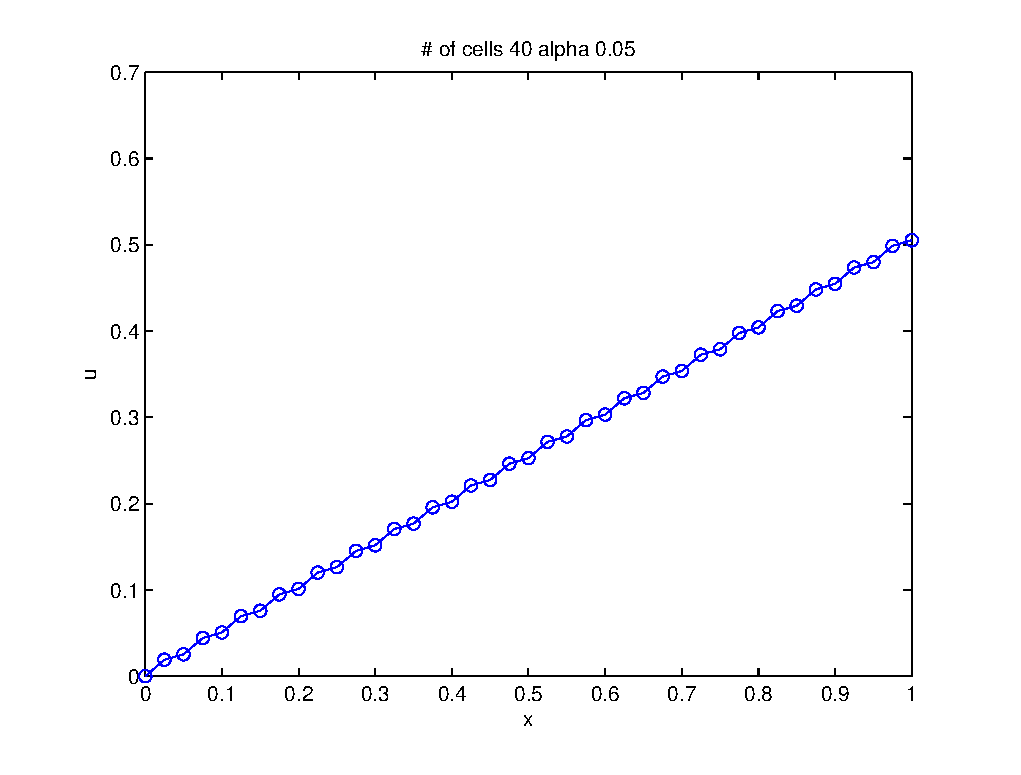
\includegraphics{conv40alpha005.eps}}
\caption{Convergence Study for $\alpha = 0.05$}\label{fig:convgfinitevolcutPC}
\end{figurehere}
\end{center}
\begin{center}
\begin{figurehere}
\scalebox{0.5}{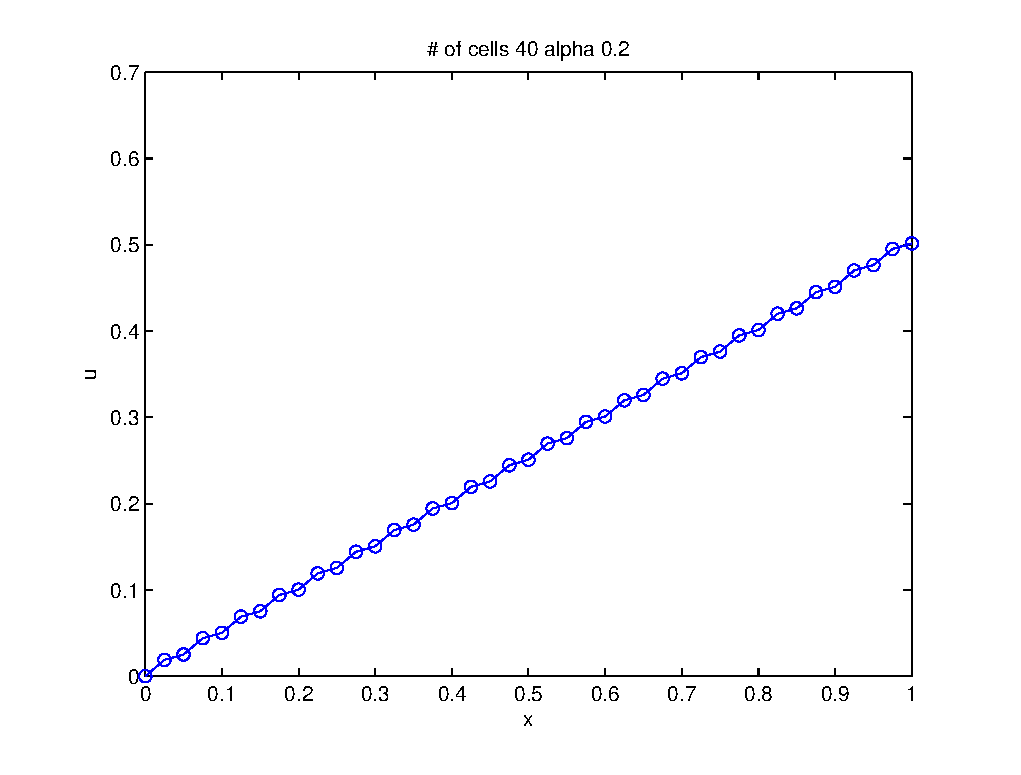
\includegraphics{40alpha02.eps}}
\scalebox{0.5}{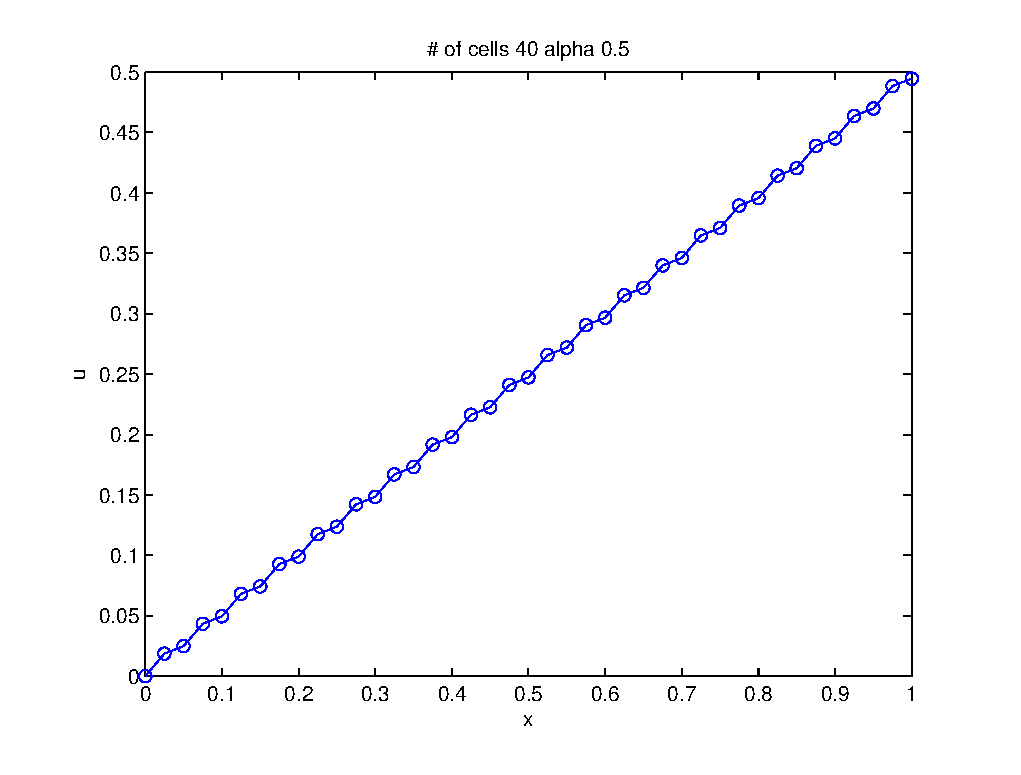
\includegraphics{40alpha05.eps}}
\scalebox{0.5}{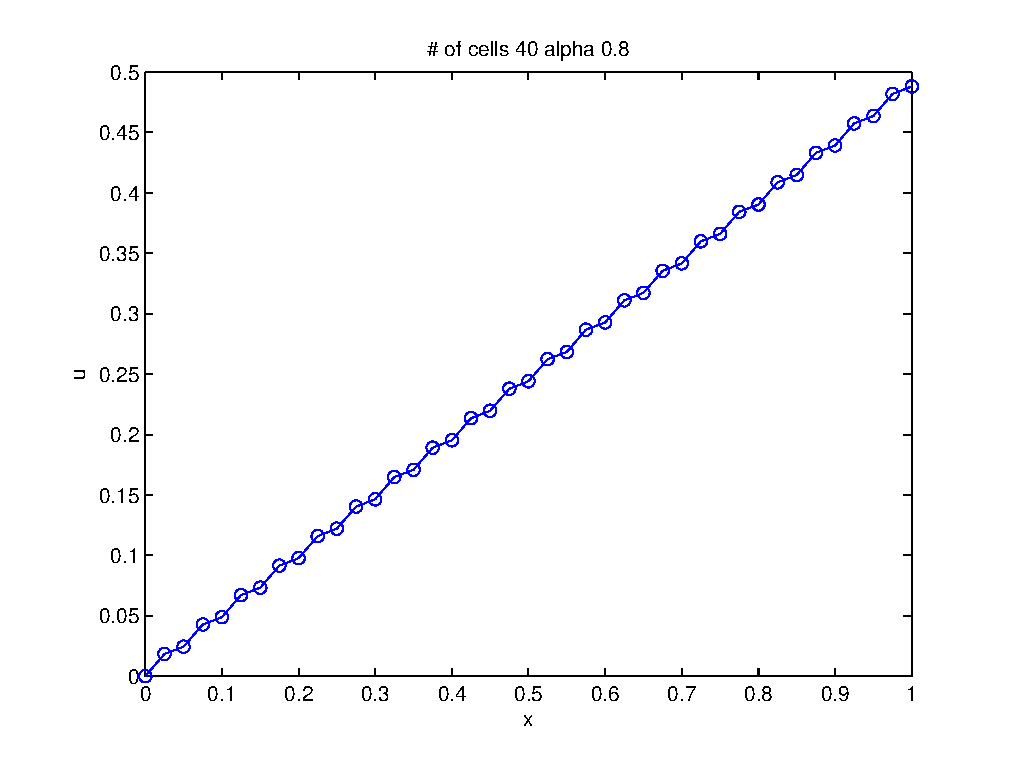
\includegraphics{40alpha08.eps}}
\caption{Solution With Cut Cell for different values of $\alpha$}\label{fig:finitevolcutPC}
\end{figurehere}
\end{center}
\subsection{Second Attempt: Finite Volume Method (Prof. Colella Approach)}\label{sec:PCCutCellTheory}
\subsubsection{Theory}
The same problem stated in (\ref{eqn:problem}) is going to be solved here. 
We obtain an equation at each centroid of a cell.
\begin{eqnarray}
\frac{\partial ^2 u}{\partial x^2}\vert_{x_{i+\frac{1}{2}}}  &=& \frac{-K}{A},\\
\Leftrightarrow \frac{1}{\Delta x}(\frac{\partial u}{\partial x}\vert_{R} -\frac{\partial u}{\partial x}\vert_{L}) &=& \frac{-K}{A},\\
\Leftrightarrow \frac{\partial u}{\partial x}\vert_{R} -\frac{\partial u}{\partial x}\vert_{L} &=&\frac{-K\Delta x}{A},
\end{eqnarray}
The first derivative at the vertices are defined as follows:
\begin{equation}\label{eqn:derivate}
\frac{\partial u}{\partial x} = \frac{1}{\Delta x}(u_{i+1} - u_{i}),
\end{equation}
where $u_{i+1}$ and $u_i$ are the displacement on the neighbor centroids to the cell (see figure \ref{fig:derivativePC}).
\begin{center}
\begin{figurehere} 
\input{derivativePC.pstex_t}
\caption{Dependency of the Derivative at the Vertex on the Centroids Values}\label{fig:derivativePC}
\end{figurehere}
\end{center}
We have an equation per control volume. At a non-boundary element, the expression for the second derivative reads:
\begin{eqnarray}
\frac{1}{\Delta x}(u_{i+1} - u_i) - \frac{1}{\Delta x}(u_{i} - u_{i-1})&=&\frac{-K\Delta x}{A},\\
\Leftrightarrow u_{i+1} - 2 u_{i} - u_{i-1}&=&\frac{-K\Delta x^2}{A},\\
\end{eqnarray}
where $i$ is the index of the centroid of the current control volume.\footnote{Note here, that this equation is exactly the same as the one obtained in section  \ref{sec:PPfinitevolume}}. the equation at the boundary elements can not be written as straightforward. We still have:
\begin{eqnarray}
\frac{\partial u}{\partial x}\vert_{R} -\frac{\partial u}{\partial x}\vert_{L} &=&\frac{-K\Delta x}{A}.
\end{eqnarray}
If we consider the left boundary of the one-dimensional domain, the term $\frac{\partial u}{\partial x}\vert_{R}$ is defined as before in equation (\ref{eqn:derivate}). The first derivative at the left boundary, i.e. $\frac{\partial u}{\partial x}\vert_{L}$, which corresponds to the end of the physical and finite volume domain, has to be determined from an interpolation over the domain end and the two first cells' centroids. the interpolation reads as follows:
\begin{eqnarray}
\frac{\partial u}{ \partial x}\vert_{L} &=& N_{1,x}(0)u_e + N_{2,x}(0)u_1 + N_{3,x}(0)u_2,\\
N_1 &=& \frac{(x-\frac{\Delta x}{2})(x - \frac{3 \Delta x}{2})}{\frac{3\Delta x^2}{4}},\\
N_2 &=& - \frac{x(x- \frac{3\Delta x}{2})}{\frac{1}{2}\Delta x^2},\\
N_3 &=& \frac{x(x-\frac{\Delta x}{2})}{\frac{3}{2}\Delta x^2},\\
N_{1,x}(x) &=& \frac{2x - 2\Delta x}{\frac{3}{4}\Delta x^2},\\
N_{2,x}(x) &=& \frac{-2x + \frac{3\Delta x}{2}}{\frac{\Delta x^2}{2}},\\
N_{3,x}(x) &=& \frac{2x - \frac{\Delta x}{2}}{\frac{3}{2}\Delta x^2},
\end{eqnarray}
where $u_e$ is the displacement prescribed at the left boundary, $u_1$ and $u_2$ are the displacements of the  cells' centroids.\\
The equation at the last cell reads:
\begin{eqnarray}
\frac{\partial u}{\partial x}\vert_{R} -\frac{\partial u}{\partial x}\vert_{L} &=&\frac{-K\alpha\Delta x}{A},
\end{eqnarray}
where $\alpha$ is the length of the physical domain compared to the cell size. The derivative to the left of the centroid is given directly by (\ref{eqn:derivate}). The derivative to the right of the centroid might fall on a vertex or at the end of the cut cell. 
The derivative at the end of the physical domain, whether it falls on a vertex or not, is obtained by:
\begin{eqnarray}
\frac{\partial u}{ \partial x}\vert_{R} &=& N_{1,x}(\frac{3}{2}\Delta x)u_{n-2} + N_{2,x}(\frac{3}{2}\Delta x)u_{n-1} + N_{3,x}(\frac{3}{2}\Delta x)\overline{u},\\
N_1 &=& \frac{(x-\Delta x)(x - (\frac{3}{2}+\alpha)\Delta x)}{(\frac{3}{2}+\alpha)\Delta x^2},\\
N_2 &=& - \frac{x(x- (\frac{3}{2}+\alpha)\Delta x)}{(\frac{1}{2}+\alpha)\Delta x^2},\\
N_3 &=& \frac{x(x-\Delta x)}{(\frac{3}{2}+\alpha)(\frac{1}{2}+\alpha)\Delta x^2},\\
N_{1,x}(x) &=& \frac{2x - (\frac{5}{2} + \alpha)\Delta x}{(\frac{3}{2}+\alpha)\Delta x^2},\\
N_{2,x}(x) &=& - \frac{2x - (\frac{3}{2}+\alpha)\Delta x}{(\frac{3}{2}+\alpha)\Delta x},\\
N_{3,x}(x) &=& \frac{2x - \Delta x}{(\frac{3}{2}+\alpha)(\frac{1}{2}+\alpha)\Delta x^2},
\end{eqnarray}
where $u_e$ is the displacement prescribed at the end of the physical domain, $u_{n-1}$ and $u_{n-2}$ are the centroids of the neighbor full cells to the last cell. 
\subsubsection{Results}
For different values of $\alpha$, the solution is given in figure \ref{fig:alphacutPC2}.
\begin{center}
\begin{figurehere}
\scalebox{0.45}{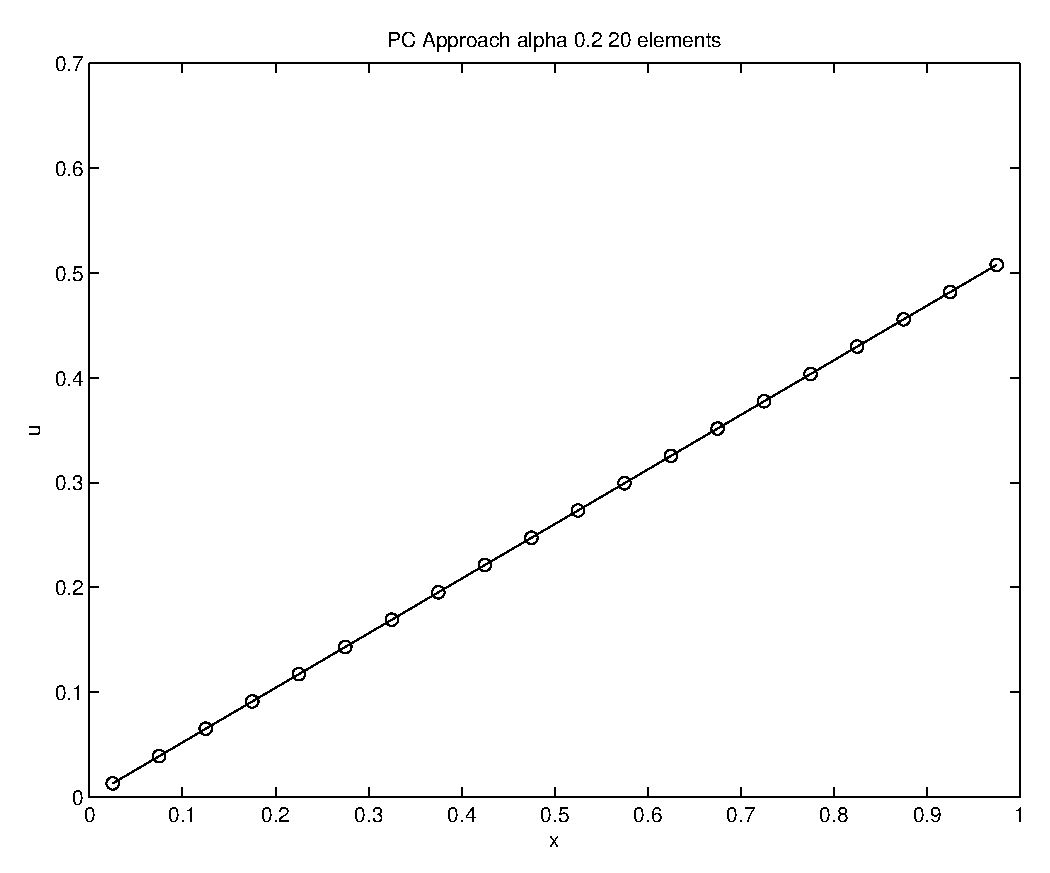
\includegraphics{PCalpha02.eps}}
\scalebox{0.45}{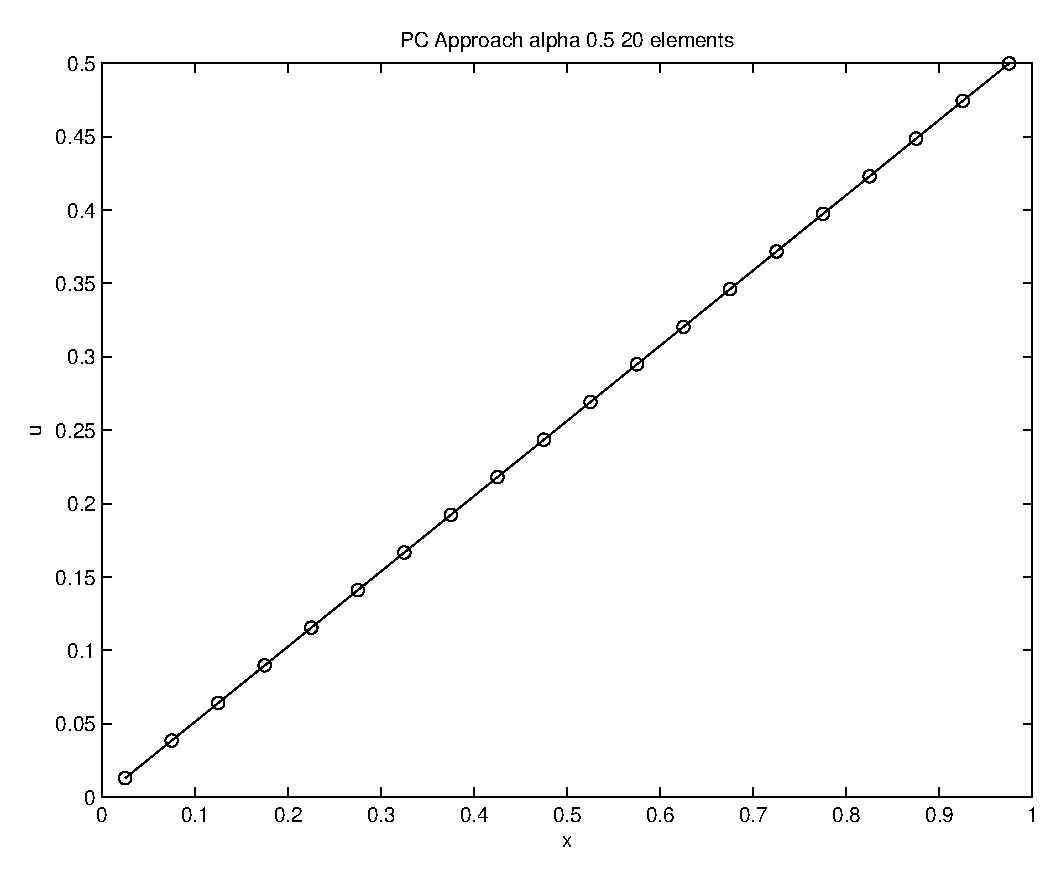
\includegraphics{PCalpha05.eps}}
\scalebox{0.45}{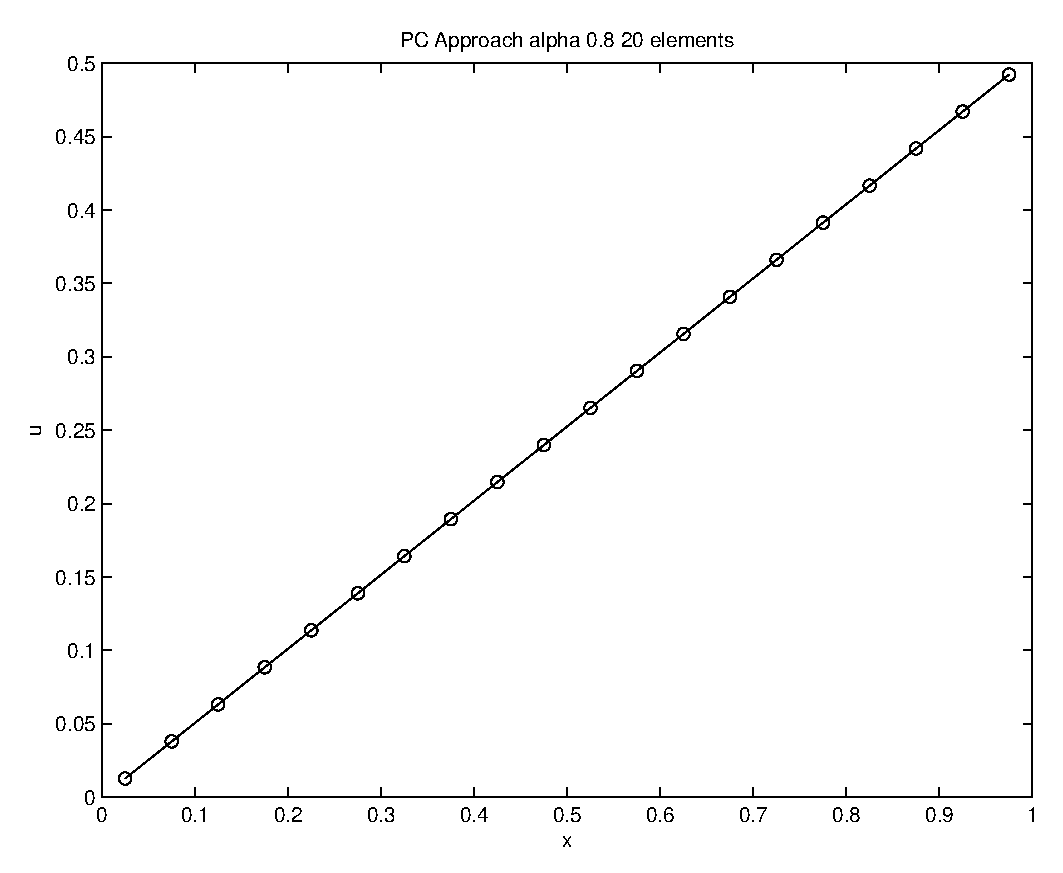
\includegraphics{PCapha08.eps}}\\
\caption{Solution for different values of $\alpha$}\label{fig:alphacutPC2}
\end{figurehere}
\end{center}
While fixing the value of $\alpha$, a convergence study with increasing the total number of elements is conducted. The results are depicted in figure \ref{fig:convgcutPC2}.
\begin{center}
\begin{figurehere}
%\centering
\scalebox{0.45}{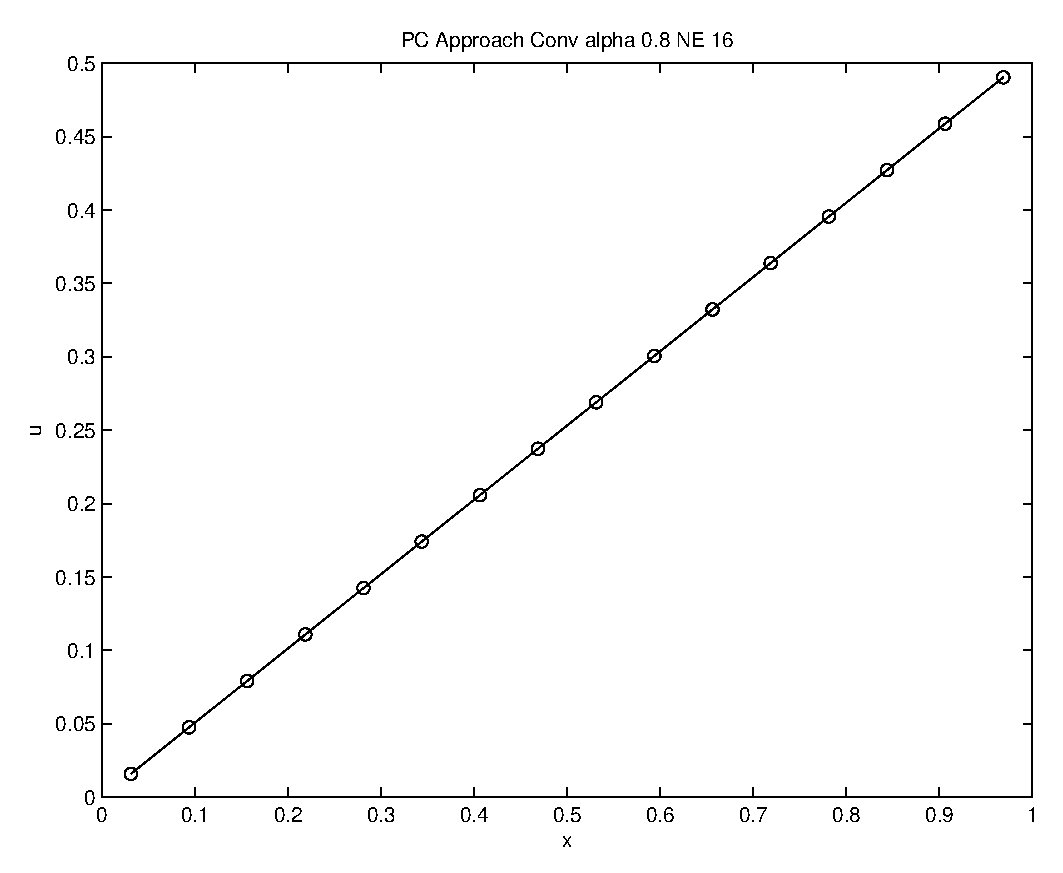
\includegraphics{convPCalpha08NE16.eps}}
\scalebox{0.45}{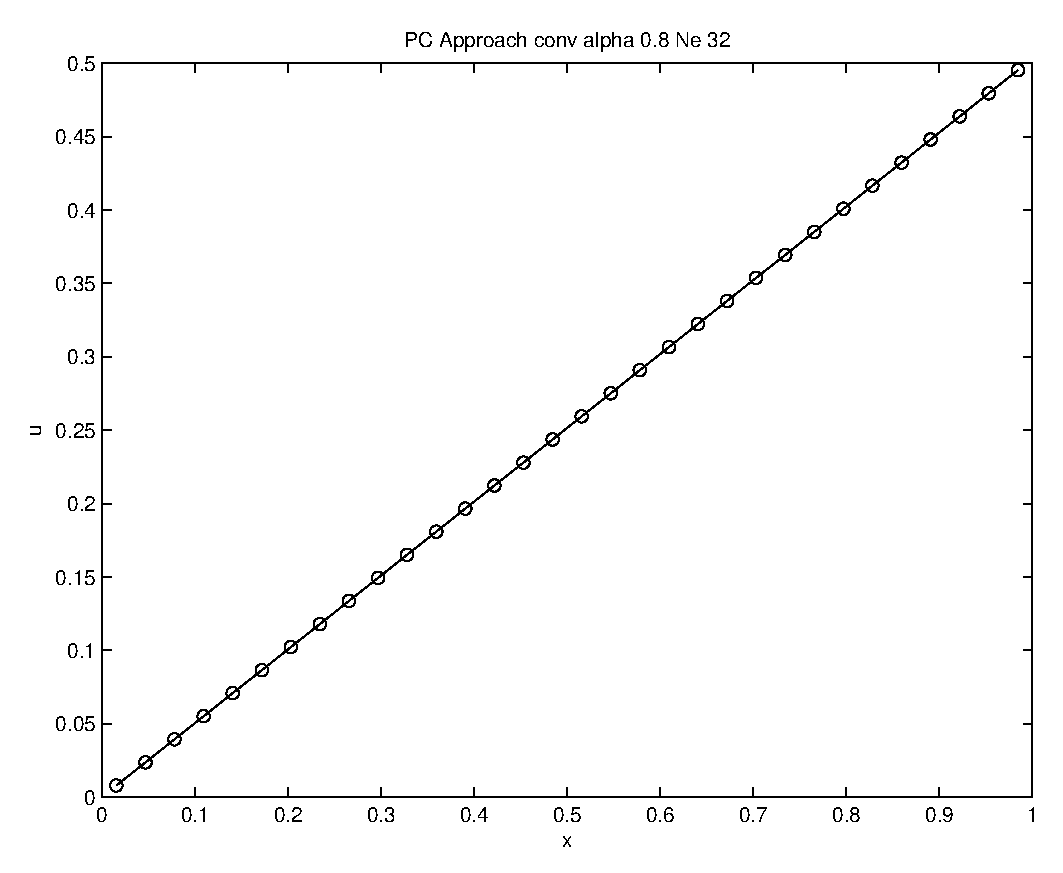
\includegraphics{convPCalpha08Ne32.eps}}
\scalebox{0.45}{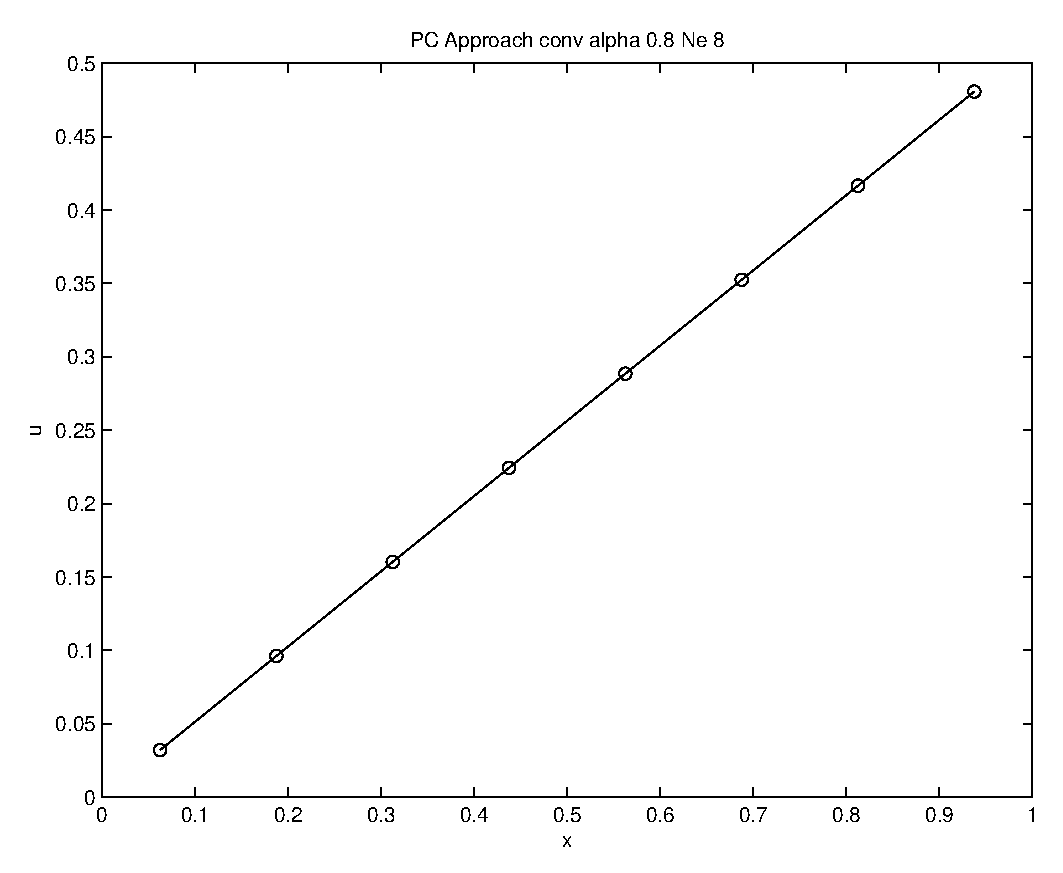
\includegraphics{convPCalpha08NE8.eps}}\\
\caption{Convergence Study for $\alpha = 0.8$}\label{fig:convgcutPC2}
\end{figurehere}
\end{center}
\subsection{Consideration of the PDE to the last element (Finite Element Method)}
\subsubsection{Results}
Problem (\ref{eqn:problem}) is going to be solved. The following parameters are used:
\begin{eqnarray}
L = 1, \hspace{0.5cm}, h = 0.25, \hspace{0.5cm}A= 3, \hspace{0.5cm}\overline{u}\vert_0 = 0.0,\\ 
\overline{u}\vert_L=0.5, \hspace{0.5cm}K = 0,\hspace{0.5cm}\alpha = 0.9,
\end{eqnarray}
where $h$ is the element size.\\
The PDE contribution is considered to the entire element, even though part of it is not included in the real physical domain. The assembling of the last element contribution to the global system helps propagating the information about the presence of a boundary condition. The boundary condition equations replace the PDE equations to the outer left and right nodes, noting that these nodes are not of interest for us because they do not really belong to the original domain. These nodes have been created to have a fair match with the finite volume method solution positions. The PDE contribution is also considered for the entire first element, even though the left part passes the actual boundary of the domain.\\ 
The solution is depicted in figure \ref{fig:femwithpde}.

\begin{center}
\begin{figurehere} 
\scalebox{0.6}{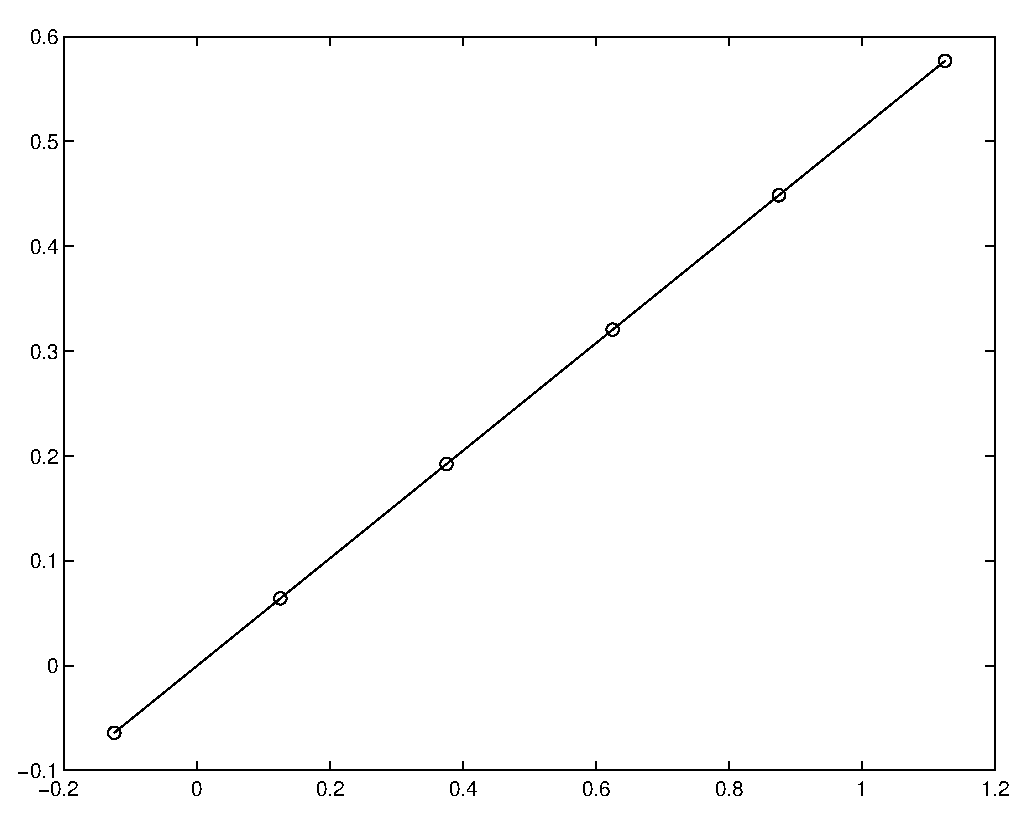
\includegraphics{femwithpde.eps}}\\
\caption{Finite Element with Consideration of PDE}\label{fig:femwithpde}
\end{figurehere}
\end{center}

\section{Comparison Of All Of The Methods}
Problem (\ref{eqn:problem}) is going to be solved using all of the methods discussed above. The following parameters are used:
\begin{eqnarray}
L = 1, \hspace{0.5cm}, ne = 4, \hspace{0.5cm}A= 3, \hspace{0.5cm}\overline{u}\vert_0 = 0.0,\\ 
\overline{u}\vert_L=0.5, \hspace{0.5cm}K = 0,\hspace{0.5cm}\alpha = 0.9.
\end{eqnarray}
We are interested in comparing the outcoming system of equations that has to be solved and hopefully recognize. \footnote{In the following, $s$ is the stiffness matrix, $f$ is the force vector and $u_n$ is the solution.}
\subsection{PP Finite Volume}
\begin{verbatim}
s =

   -4.0000    1.3333         0         0
    1.0000   -2.0000    1.0000         0
         0    1.0000   -2.0000    1.0000
         0         0    1.4286   -5.0000
\end{verbatim}
\begin{verbatim}
f =

         0
         0
         0
   -1.7857
\end{verbatim}
The unknowns are at the centroids of the volumes:
\begin{verbatim}
u_n =

    0.0641
    0.1923
    0.3205
    0.4487
\end{verbatim}
\subsection{PC Finite Volume}
\begin{verbatim}
s =

  -16.0000    5.3333         0         0
    1.0000   -2.0000    1.0000         0
         0    1.0000   -2.0000    1.0000
         0    2.3333   -2.8571   -4.0000
\end{verbatim}
\begin{verbatim}
f =

         0
         0
         0
   -2.2619
\end{verbatim}
The unknowns are at the centroids of the volumes:
\begin{verbatim}
u_n =

    0.0641
    0.1923
    0.3205
    0.4487
\end{verbatim}
\subsection{Finite Element 2 Elements Coupling}
Before application of the left boundary conditions:
\begin{verbatim}
s =

   12.0000  -12.0000         0         0         0
  -12.0000   24.0000  -12.0000         0         0
         0  -12.0000   24.0000  -12.0000         0
         0         0  -12.0000   12.0000         0
         0         0   -0.0526    0.2222    1.0000
\end{verbatim}
\begin{verbatim}
f =

         0
         0
         0
         0
    0.5848
\end{verbatim}
After application of the left boundary conditions:
\begin{verbatim}
s =

   24.0000  -12.0000         0         0
  -12.0000   24.0000  -12.0000         0
         0  -12.0000   12.0000         0
         0   -0.0526    0.2222    1.0000
\end{verbatim}
\begin{verbatim}
f =

         0
         0
         0
    0.5848
\end{verbatim}
The unknowns are at the nodes.
\begin{verbatim}
u_n =

         0
         0
         0
    0.5848
\end{verbatim}
\subsection{Finite Element 3 Elements Coupling}
Before application of the left boundary conditions:
\begin{verbatim}
s =

   12.0000  -12.0000         0         0         0
  -12.0000   24.0000  -12.0000         0         0
         0  -12.0000   24.0000  -12.0000         0
         0         0  -12.0000   12.0000         0
         0    0.0285   -0.1755    0.3705    1.1115
\end{verbatim}
\begin{verbatim}
f =

         0
         0
         0
         0
    0.5000
\end{verbatim}
After application of the left boundary conditions:
\begin{verbatim}
s =

   24.0000  -12.0000         0         0
  -12.0000   24.0000  -12.0000         0
         0  -12.0000   12.0000         0
    0.0285   -0.1755    0.3705    1.1115
\end{verbatim}
\begin{verbatim}
f =

         0
         0
         0
    0.5000
\end{verbatim}
The unknowns are at the nodes.
\begin{verbatim}
u_n =

         0
         0
         0
    0.4498
\end{verbatim}
\subsection{Finite Element Tranair Approach With Consideration of the DE Contribution}
\subsubsection{Penalty Method}
The solution is calculated with a penalty parameter of $1000$.\\
Before application of the left boundary conditions:
\begin{verbatim}
s =

  -12.0000   12.0000         0         0         0
   12.0000  -24.0000   12.0000         0         0
         0   12.0000  -24.0000   12.0000         0
         0         0   12.0000  169.9759  257.0866
         0         0         0  257.0866  303.8509
\end{verbatim}
\begin{verbatim}
f =

         0
         0
         0
  219.5312
  280.4688
\end{verbatim}
After application of the left boundary conditions:
\begin{verbatim}
s =

  -24.0000   12.0000         0         0
   12.0000  -24.0000   12.0000         0
         0   12.0000  169.9759  257.0866
         0         0  257.0866  303.8509
\end{verbatim}
\begin{verbatim}
f =

         0
         0
  219.5312
  280.4688
\end{verbatim}
The unknowns are at the nodes.
\begin{verbatim}
u_n =
         0
    0.1498
    0.2996
    0.4494
    0.5428
\end{verbatim}
It is to be noted here that the finite element method solution is not accurate. But also, we could not compare correctly because of the misplacement of the unknowns in the methods, i.e. the finite element method positions the unknowns at cell edges and the finite volume method positions them at the cell centers. This has to be taken into account in future investigations.
\subsubsection{Lagrange Multiplier}
The Lagrange multiplier approach has not been implemented, because it is just going to be a different method for imposing the Dirichlet boundary conditions, which we know that it is going to work. We do not see any urgent purpose for implementing this because it would not lead to new conclusions regarding our study. 
\subsection{Remarks}
It is to be noted here that the finite element method solution is not accurate. But also, we could not compare correctly because of the misplacement of the unknowns in the methods, i.e. the finite element method positions the unknowns at cell edges and the finite volume method positions them at the cell centers. This has to be taken into account in future investigations.Therefore, one can force the position of the unknowns of the finite element method at the cell centers. For this purpose, one expands the domain to the right and to the left to maintain the same mesh size for all methods (see figure \ref{fig:femVSfvm}).
\begin{center}
\begin{figurehere} 
{\input{fvmVSfem.pstex_t }}\\
\caption{Position of the unknowns: Finite Volume Method (upper), Finite Element Method (bottom)}\label{fig:femVSfvm}
\end{figurehere}
\end{center}
\section{Comparisons: New Attempt}\label{sec:comparisonNewAttempt}
Problem (\ref{eqn:problem}) is going to be solved using all of the methods discussed above. The following parameters are used:
\begin{eqnarray}
L = 1, \hspace{0.5cm}, h = 0.25, \hspace{0.5cm}A= 3, \hspace{0.5cm}\overline{u}\vert_0 = 0.0,\\ 
\overline{u}\vert_L=0.5, \hspace{0.5cm}K = 0,\hspace{0.5cm}\alpha = 0.9,
\end{eqnarray}
where $h$ is the element size.
\subsection{PP Finite Volume}
\begin{verbatim}
s =

   -4.0000    1.3333         0         0
    1.0000   -2.0000    1.0000         0
         0    1.0000   -2.0000    1.0000
         0         0    1.4286   -5.0000
\end{verbatim}
\begin{verbatim}
f =

         0
         0
         0
   -1.7857
\end{verbatim}
The unknowns are at the centroids of the volumes:
\begin{verbatim}
u_n =

    0.0641
    0.1923
    0.3205
    0.4487
\end{verbatim}
\subsection{Scaled PP Finite Volume}
After obtaining the finite element solution, we want to fairly compare with the vector and matrix entries of the finite volume method to hopefully extract an analogy. The finite volume system is scaled by $12$.
\begin{verbatim}
s =

   -48.0000    15.9996          0          0
    12.0000   -24.0000    12.0000          0
         0     12.0000   -24.0000    12.0000
         0         0      17.1432   -60.0000
\end{verbatim}
\begin{verbatim}
f =

          0
          0
          0
   -21.4284
\end{verbatim}
The unknowns are at the centroids of the volumes:
\begin{verbatim}
u_n =

    0.0641
    0.1923
    0.3205
    0.4487
\end{verbatim}
\subsection{PC Finite Volume}
\begin{verbatim}
s =

  -16.0000    5.3333         0         0
    1.0000   -2.0000    1.0000         0
         0    1.0000   -2.0000    1.0000
         0    2.3333   -2.8571   -4.0000
\end{verbatim}
\begin{verbatim}
f =

         0
         0
         0
   -2.2619
\end{verbatim}
The unknowns are at the centroids of the volumes:
\begin{verbatim}
u_n =

    0.0641
    0.1923
    0.3205
    0.4487
\end{verbatim}
\subsection{Scaled PC Finite Volume}
After obtaining the finite element solution, we want to fairly compare the vector and matrix entries to hopefully extract an analogy. The finite volume system is scaled by $12$.
\begin{verbatim}
s =

  -192.0000    63.9996          0          0
    12.0000   -24.0000    12.0000          0
         0     12.0000   -24.0000    12.0000
         0     27.9996   -34.2852   -48.0000
\end{verbatim}
\begin{verbatim}
f =

          0
          0
          0
   -27.1428
\end{verbatim}
The unknowns are at the centroids of the volumes:
\begin{verbatim}
u_n =

    0.0641
    0.1923
    0.3205
    0.4487
\end{verbatim}
\subsection{Finite Element 2 Elements Coupling With PDE contribution}
\begin{verbatim}
s =

   -3.0000   -6.0000    1.0000         0         0         0
  -12.0000   24.0000  -12.0000         0         0         0
         0  -12.0000   24.0000  -12.0000         0         0
         0         0  -12.0000   24.0000  -12.0000         0
         0         0         0  -12.0000   24.0000  -12.0000
         0         0         0   -0.4286    3.0000    1.0000
\end{verbatim}
\begin{verbatim}
f =

         0
         0
         0
         0
         0
    1.7857
\end{verbatim}
The unknowns are at the cell centers.
\begin{verbatim}
u_n =

   -0.0641
    -------
    0.0641
    0.1923
    0.3205
    0.4487
    -------
    0.5769
\end{verbatim}
\subsection{Finite Element Tranair Approach}
\begin{verbatim}
s =

  -12.0000   12.0000         0         0         0         0
   12.0000  -24.0000   12.0000         0         0         0
         0   12.0000  -24.0000   12.0000         0         0
         0         0   12.0000  -24.0000   12.0000         0
         0         0         0   12.0000  236.3819  252.3994
         0         0         0         0  252.3994  246.8194

\end{verbatim}
\begin{verbatim}
f =

         0
         0
         0
         0
  250.3906
  249.6094
\end{verbatim}
The unknowns are at the cell centers.
\begin{verbatim}
u_n =

   -0.0528
    ------
    0.0528
    0.1584
    0.2640
    0.3697
    -------
    0.6333
\end{verbatim}
The array entries presented above have been consistently implemented such that negative definiteness is given. For the sake of convenience, the signs have been changed such that positive definiteness is obtained. 
\section{Comparison Study}
After looking at the results obtained in section \ref{sec:comparisonNewAttempt}, one is intrigued to know about the extend of the similarities between the methods used, i.e. one wants to compare as many digits as possible in the different solutions.\\
Since the finite element approach using a two-elements-coupling and considering the partial differential equation contribution to the entire physical domain led to an exactly same answer as the finite volume one, we are curious to know about the extend of correctness as well as the effect of the ratio $\alpha$ on the solution. \\
Now, the domain is extended to a half of the element size to the left to match the finite volume unknowns position. Therefore, there has been introducted a similar ratio to $\alpha$ that does always have the value of $0.5$. It would also be good to know if the extension of the left boundary of the finite element domain does affect the solution.
Problem (\ref{eqn:problem}) is going to be solved using all of the methods discussed above. The following parameters are used:
\begin{eqnarray}
L = 1, \hspace{0.5cm}, h = 0.25, \hspace{0.5cm}A= 3, \hspace{0.5cm}\overline{u}\vert_0 = 0.0,\\ 
\overline{u}\vert_L=0.5, \hspace{0.5cm}K = 0,\hspace{0.5cm}\alpha = 0.9,
\end{eqnarray}
where $h$ is the element size.
\subsection{PP Finite Volume}
\begin{verbatim}
s =

    4.0000   -1.3333         0         0
   -1.0000    2.0000   -1.0000         0
         0   -1.0000    2.0000   -1.0000
         0         0   -1.4286    5.0000
\end{verbatim}
\begin{verbatim}
f =

         0
         0
         0
    1.7857
\end{verbatim}
The unknowns are at the centroids of the volumes:
\begin{verbatim}
u_n =

   0.064102564102564
   0.192307692307692
   0.320512820512820
   0.448717948717949
\end{verbatim}'
The results are depicted in figure \ref{fig:studyfiniteVolPP}.
\begin{figure} 
\centering
\scalebox{0.65}{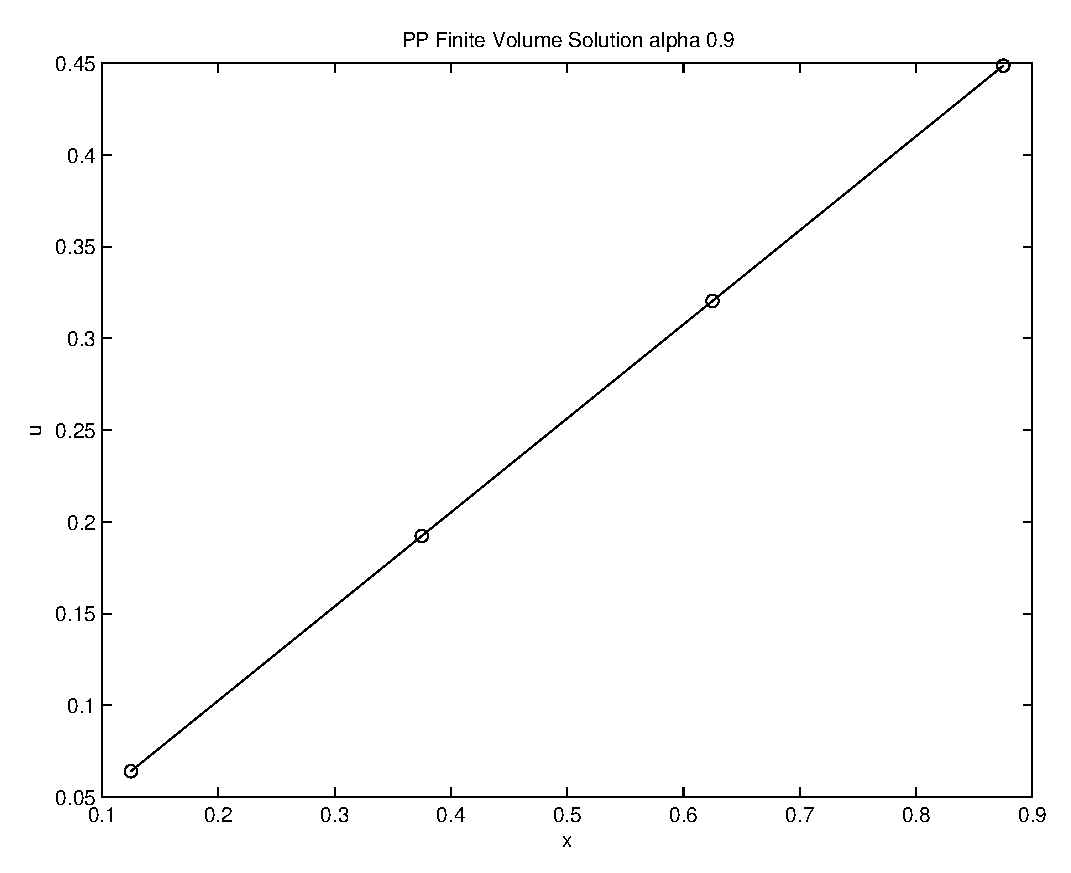
\includegraphics{study_PP.eps}}\\
\caption{Solution with Finite Volume PP}\label{fig:studyfiniteVolPP}
\end{figure}
\subsection{PC Finite Volume}
\begin{verbatim}
s =

   16.0000   -5.3333         0         0
   -1.0000    2.0000   -1.0000         0
         0   -1.0000    2.0000   -1.0000
         0   -2.3333    2.8571    4.0000
\end{verbatim}
\begin{verbatim}
f =

         0
         0
         0
    2.2619
\end{verbatim}
The unknowns are at the centroids of the volumes:
\begin{verbatim}
u_n =

   0.064102564102564
   0.192307692307692
   0.320512820512821
   0.448717948717949
\end{verbatim}
The results are depicted in figure \ref{fig:studyfiniteVolPC}.
\begin{figurehere} 
\centering
\scalebox{0.65}{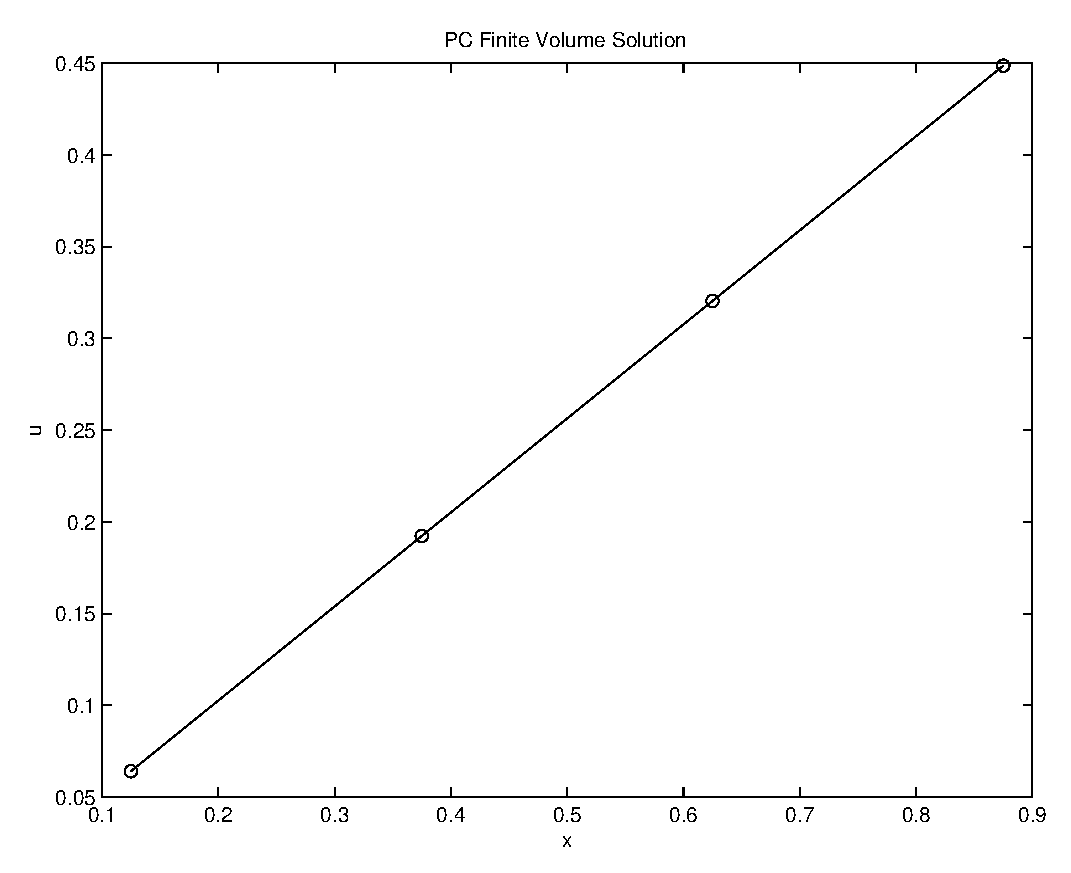
\includegraphics{study_PC.eps}}\\
\caption{Solution with Finite Volume PC}\label{fig:studyfiniteVolPC}
\end{figurehere}
\subsection{Finite Element 2 Elements Coupling With Full PDE contribution}
The PDE contribution is considered to the entire first and last element as if they would have belonged to the physical domain.
\begin{verbatim}
s =

    3.0000    6.0000   -1.0000         0         0         0
  -12.0000   24.0000  -12.0000         0         0         0
         0  -12.0000   24.0000  -12.0000         0         0
         0         0  -12.0000   24.0000  -12.0000         0
         0         0         0  -12.0000   24.0000  -12.0000
         0         0         0   -0.4286    3.0000    1.0000
\end{verbatim}
\begin{verbatim}
f =

         0
         0
         0
         0
         0
    1.7857
\end{verbatim}
The unknowns are at the cell centers.
\begin{verbatim}
u_n =

  -0.064102564102564
   -----------------
   0.064102564102564
   0.192307692307693
   0.320512820512821
   0.448717948717950
   -----------------
   0.576923076923078
\end{verbatim}
The results are depicted in figure \ref{fig:studyfullPDE}.
\begin{center}
\begin{figurehere} 
\scalebox{0.75}{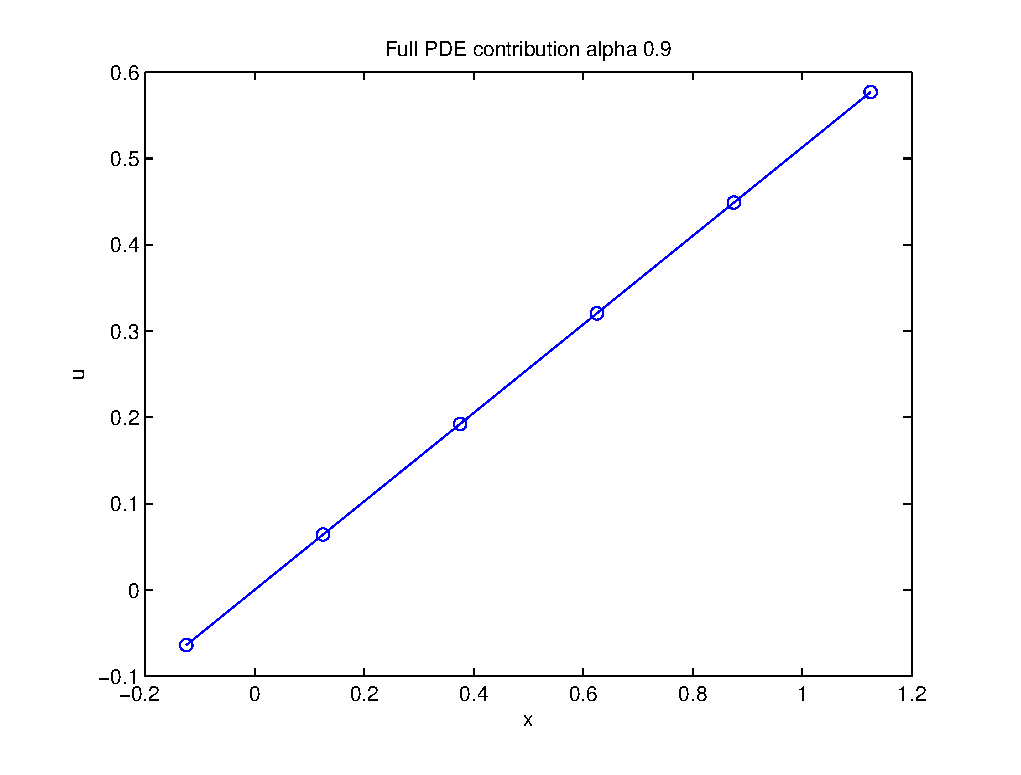
\includegraphics{study_fullPDE.eps}}\\
\caption{Solution with Full PDE Contribution}\label{fig:studyfullPDE}
\end{figurehere}
\end{center}
\subsection{Finite Element 2 Elements Coupling With Scaled PDE contribution}
The ratio of the physical domain length to the entire domain length is used to scale the PDE contribution to the first and last element as they do both expand the actual boundaries.
\begin{verbatim}
s =

    3.0000    6.0000   -1.0000         0         0         0
   -6.0000   18.0000  -12.0000         0         0         0
         0  -12.0000   24.0000  -12.0000         0         0
         0         0  -12.0000   24.0000  -12.0000         0
         0         0         0  -12.0000   14.4000   -2.4000
         0         0         0   -0.4286    3.0000    1.0000
\end{verbatim}
\begin{verbatim}
f =

         0
         0
         0
         0
         0
    1.7857
\end{verbatim}
The unknowns are at the cell centers.
\begin{verbatim}
u_n =

  -0.104263206672845
   -----------------
   0.081093605189991
   0.173772011121409
   0.266450417052827
   0.359128822984245
   -----------------
   0.822520852641336
\end{verbatim}
The results are depicted in figure \ref{fig:studypartialPDE}.
\begin{center}
\begin{figurehere}[p]
\scalebox{0.75}{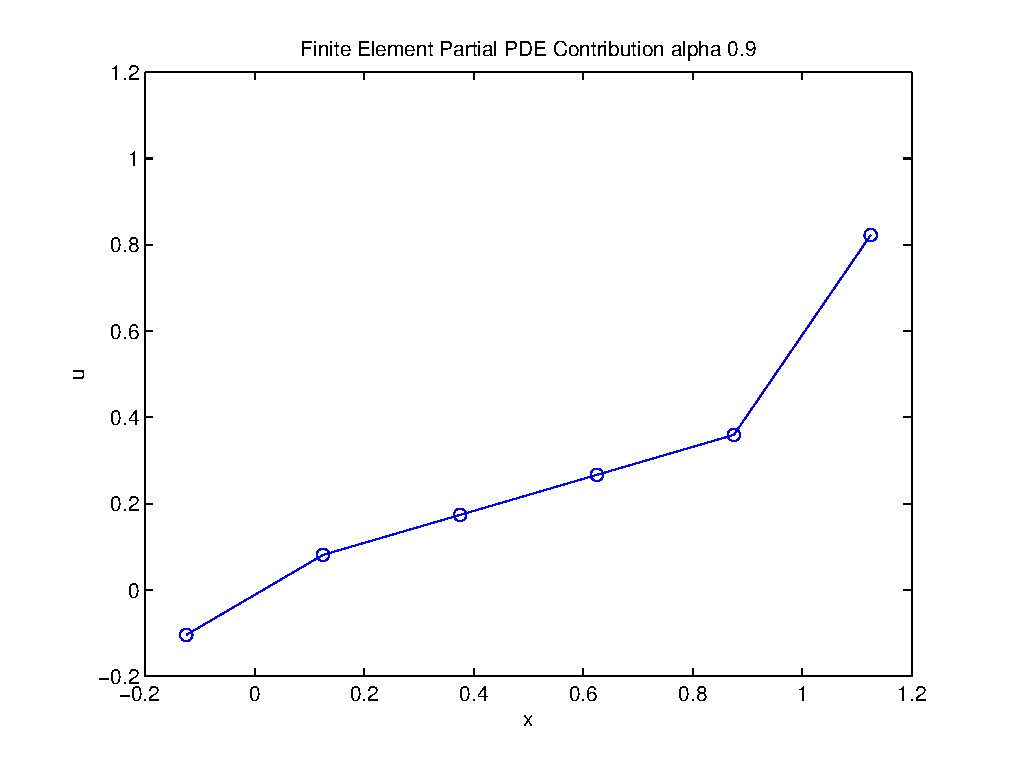
\includegraphics{study_partialPDE.eps}}\\
\caption{Solution with Partial PDE Contribution}\label{fig:studypartialPDE}
\end{figurehere}
\end{center}
\subsection{Finite Element Tranair Approach}
\begin{verbatim}
s =

    3.0000    6.0000   -1.0000         0         0         0
   -6.0000   18.0000  -12.0000         0         0         0
         0  -12.0000   24.0000  -12.0000         0         0
         0         0  -12.0000   24.0000  -12.0000         0
         0         0         0  -12.0000 -236.3819 -252.3994
         0         0         0         0 -252.3994 -246.8194

\end{verbatim}
\begin{verbatim}
f =

         0
         0
         0
         0
 -250.3906
 -249.6094
\end{verbatim}
The unknowns are at the cell centers.
\begin{verbatim}
u_n =

  -0.110097737785369
   -----------------
   0.085631573833065
   0.183496229642282
   0.281360885451498
   0.379225541260715
   -----------------
   0.623504896972005
\end{verbatim}
The results are depicted in figure \ref{fig:studytranair}.\\
\begin{center}
\begin{figurehere} 
\scalebox{0.75}{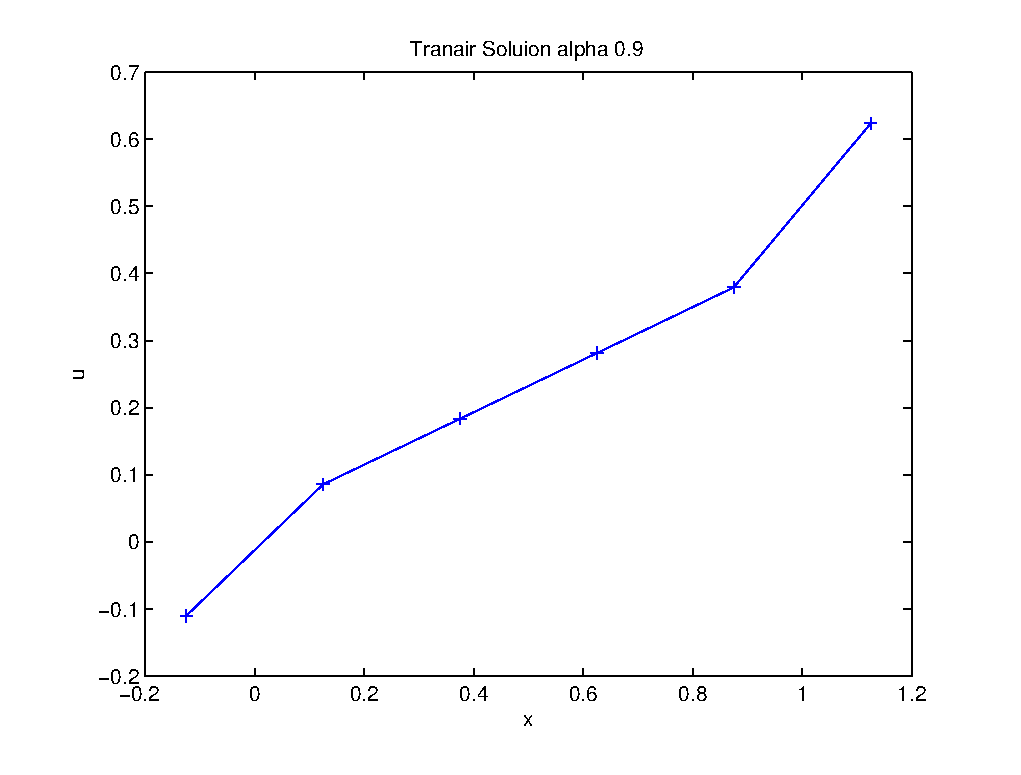
\includegraphics{study_tranair.eps}}\\
\caption{Solution with Tranair Approach}\label{fig:studytranair}
\end{figurehere}
\end{center}
Positive definiteness of the system is convenient. We notice the negative entries on the last two rows of the stiffness matrix. Instead of adding the penalty terms, which collapse at the end to zero, the entries can be subtracted, i.e.
\begin{equation*}
- \int Au_{,x}\xi_{,x}\intd x + \int K \xi \intd x -  (\xi(u-\overline{u}))\vert_{L}= 0.
\end{equation*}
Therefore, we obtain positive diagonal entries, but a slight change in the solution, which will disappear when the element size decreases..\\
\begin{verbatim}
s =

    3.0000    6.0000   -1.0000         0         0         0
   -6.0000   18.0000  -12.0000         0         0         0
         0  -12.0000   24.0000  -12.0000         0         0
         0         0  -12.0000   24.0000  -12.0000         0
         0         0         0  -12.0000  265.1819  247.5994
         0         0         0         0  247.5994  251.6194
\end{verbatim}
\begin{verbatim}
f =

         0
         0
         0
         0
  250.3906
  249.6094
\end{verbatim}
The unknowns are at the cell centers.
\begin{verbatim}
u_n =

  -0.109582971396014
   -----------------
   0.085231199974678
   0.182638285660024
   0.280045371345370
   0.377452457030717
   -----------------
   0.620589674815624
\end{verbatim}
\subsection{Comments}
It is interesting to see that the full consideration of the PDE to the last and first elements in the finite element approach leads to exactly the same answer as in the finite volume method. When multiplying the PDE contributions with a ratio $\alpha$, the first and last finite elements are still considered entirely but with a partial stiffness. We therefore obtain a nonhomogeneous material distribution that leads to the nonlinearity we see in the solution both obtained by the Tranair approach and the finite element method with partial PDE contribution. 
\subsection{Finite Element 2 Elements Coupling With Full PDE contribution Linear BC Interpolation}
At the beginning of this document, we have researched the use of different level of interpolation to enforce the boundary conditions. All levels have led to wrong results because we were considering the partially physical elements to be made of foam, i.e. they do not have any stiffness so no contribution to the PDE assembling. Now, we discovered that the full contribution of the PDE to the first and last elements do lead to a correct result, the same obtained from the finite volume method. 
In the one-dimensional case, the quadratic interpolation is computationally cheap, but extending this to multi-dimensions would be quite a bit of an effort. So, what if we replace the quadratic interpolation with a linear one and consistently consider the full contribution from the PDE?
\begin{verbatim}
s =

   -0.5000   -0.5000         0         0         0         0
  -12.0000   24.0000  -12.0000         0         0         0
         0  -12.0000   24.0000  -12.0000         0         0
         0         0  -12.0000   24.0000  -12.0000         0
         0         0         0  -12.0000   24.0000  -12.0000
         0         0         0         0    0.6000    0.4000
\end{verbatim}
\begin{verbatim}
f =

         0
         0
         0
         0
         0
    0.5000
\end{verbatim}
The unknowns are at the cell centers.
\begin{verbatim}
u_n =

  -0.064102564102564
   -----------------
   0.064102564102564
   0.192307692307692
   0.320512820512820
   0.448717948717949
   -----------------
   0.576923076923077
\end{verbatim}
The results are depicted in figure \ref{fig:studyfullPDElinearInter}.
\begin{center}
\begin{figurehere} 
\scalebox{0.65}{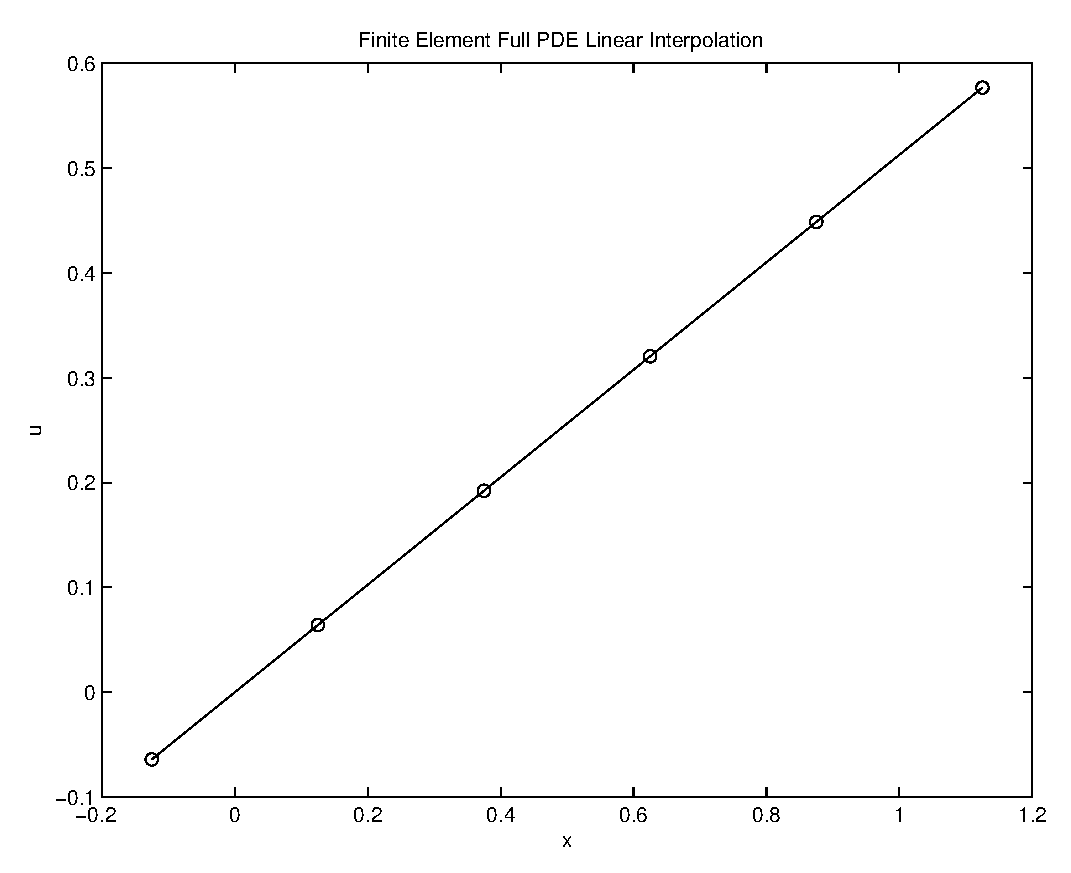
\includegraphics{studyfemfulllinear.eps}}\\
\caption{Solution with Full PDE Contribution Linear BC Interpolation}\label{fig:studyfullPDElinearInter}
\end{figurehere}
\end{center}
\section{New Problem : Quadratic Solution}
The solution we were looking at in the comparison studies was a purely linear solution due the lack of gravity, i.e. the right hand side $K$ was zero. The linear interpolation for imposing the boundary conditions seemed to work, but we guess that this approach would fail if the solution itself would be quadratic. Therefore, we want to explore the choice of the level of interpolation depending on the solution type. \\
The problem we want to solve reads now: 
\begin{eqnarray}
L = 1, \hspace{0.5cm}, h = 0.25, \hspace{0.5cm}A= 3, \hspace{0.5cm}\overline{u}\vert_0 = 0.0,\\ 
\overline{u}\vert_L=0.5, \hspace{0.5cm}K = -3,\hspace{0.5cm}\alpha = 0.9,
\end{eqnarray}
where $h$ is the element size.\\
For reference, the finite volume solution is:
\begin{verbatim}
u_n =

   0.010977564102564
   0.079807692307692
   0.211137820512821
   0.404967948717949,
\end{verbatim}
and depicted in figure \ref{fig:quadsolfv}.\\
\begin{center}
\begin{figurehere}
\scalebox{0.65}{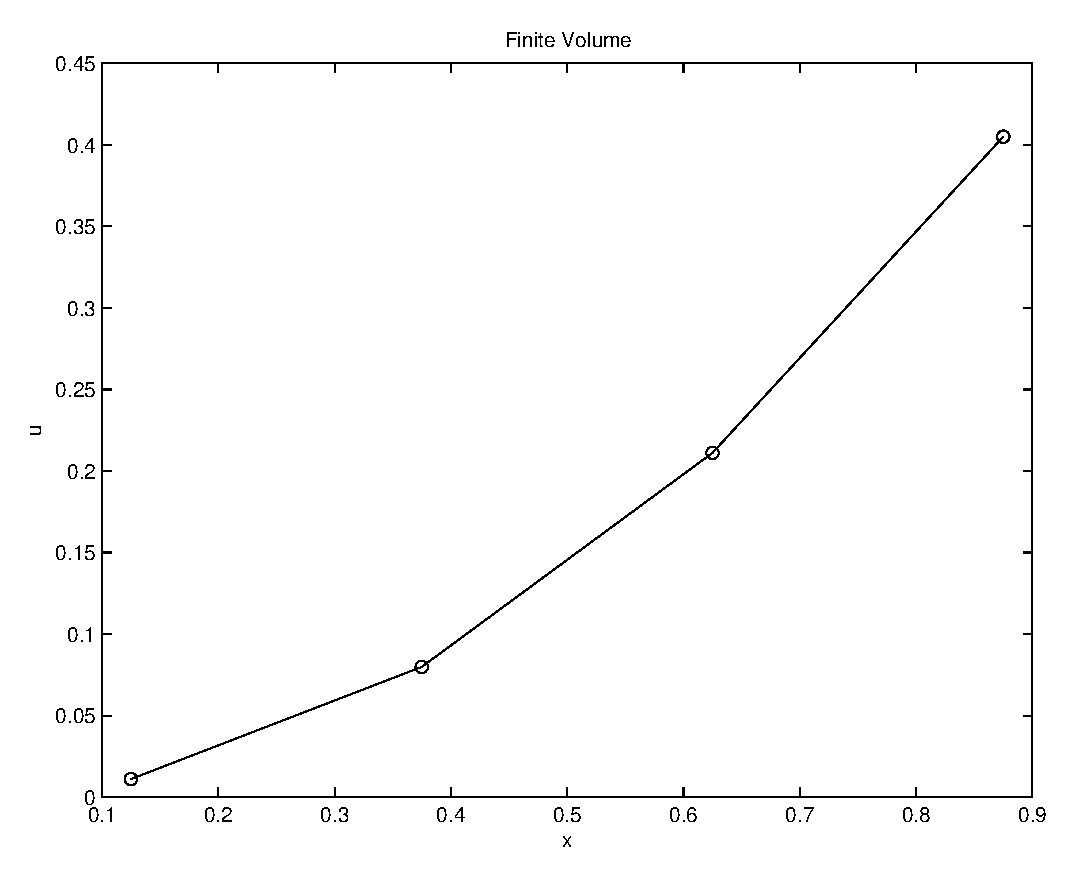
\includegraphics{quadsolfv.eps}}\\
\caption{Quadratic Solution of Finite Volume Method}\label{fig:quadsolfv}
\end{figurehere}
\end{center}
Imposing the boundary conditions means a linear interpolation leads to the following solution:
\begin{verbatim}
u_n =

  -0.003205128205128
   -----------------
   0.003205128205128
   0.072115384615385
   0.203525641025641
   0.397435897435897
   -----------------
   0.653846153846154,
\end{verbatim}
that is depicted in figure \ref{fig:quadsollininter}.\\
\begin{center}
\begin{figurehere} 
\scalebox{0.65}{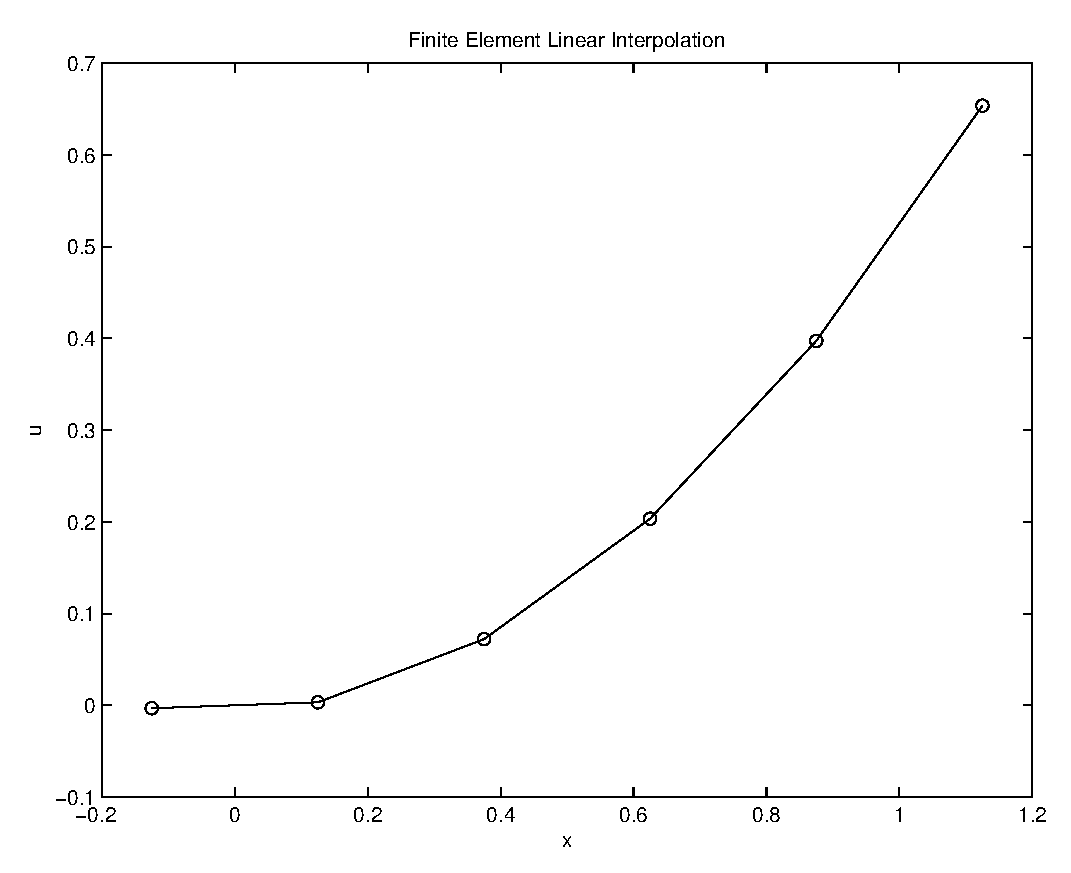
\includegraphics{quadsollininter.eps}}\\
\caption{Quadratic Solution of Finite Element Method With Linear Interpolation of Boundary Conditions}\label{fig:quadsollininter}
\end{figurehere}
\end{center}
The linear interpolation results are off in the order of $10^{-2}$. This is sceptical because the error could be higher if the solution curvature would be higher.\\
Alternatively, using a quadratic interpolation for the boundary conditions, we obtain the following results:
\begin{verbatim}
u_n =

   0.004647435897436
   -----------------
   0.010977564102564
   0.079807692307693
   0.211137820512821
   0.404967948717950
   -----------------
   0.661298076923078
\end{verbatim}
which are exactly the same as the one obtained from the finite volume method.
The solution is depicted in figure \ref{fig:quadsolquadinter}.\\
\begin{center}
\begin{figurehere}
\scalebox{0.65}{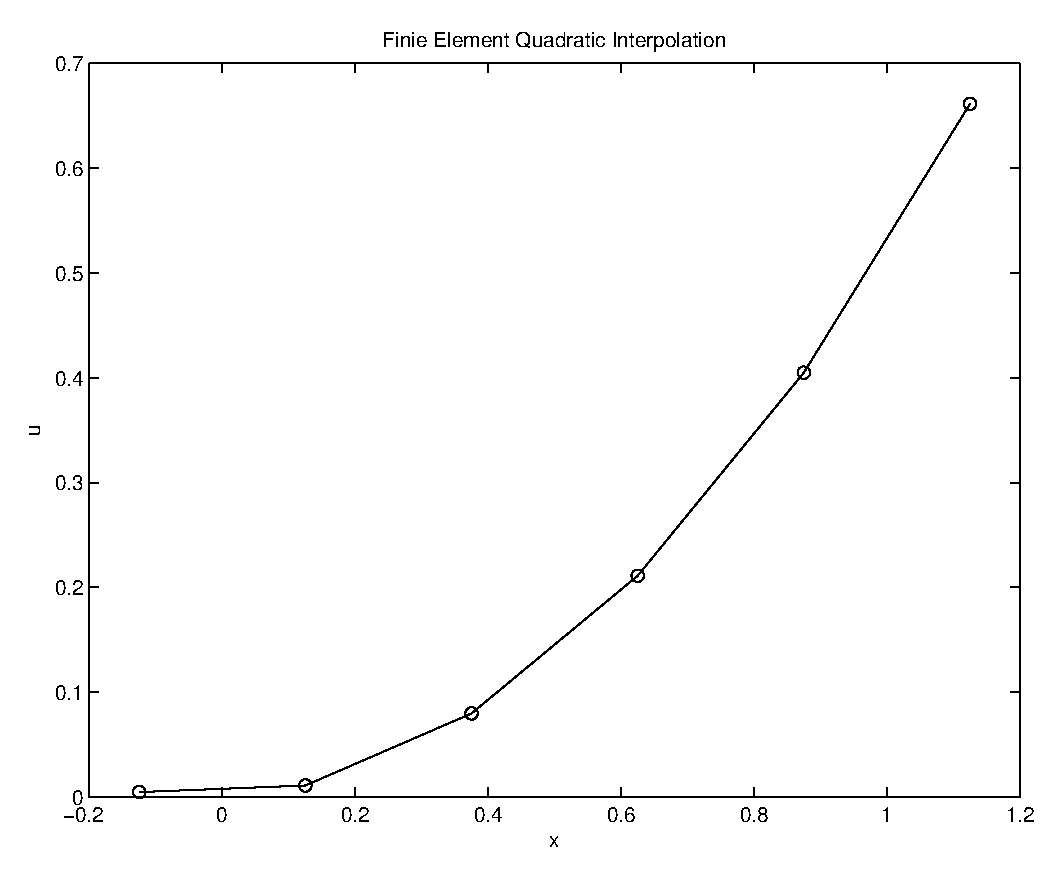
\includegraphics{quadsolquadinter.eps}}\\
\caption{Quadratic Solution of Finite Element Method With Quadratic Interpolation of Boundary Conditions}\label{fig:quadsolquadinter}
\end{figurehere}
\end{center}
\section{Neumann Boundary Conditions}
In the previous section, the idea of cut cells has been applied to boundaries with imposed Dirichlet boundary conditions. Now, we want to explore the treatment of Neumann boundary conditions within the finite element cut cell approach.
The problem to be solved is slightly modified:
\begin{eqnarray}
L = 1, \hspace{0.5cm}, h = 0.05, \hspace{0.5cm}A= 3, \hspace{0.5cm}\overline{u}\vert_0 = 0.0,\\ 
\overline{\frac{\partial u}{\partial x}}\vert_L=0.5, \hspace{0.5cm}K = -3,\hspace{0.5cm}\alpha = 0.9,
\end{eqnarray}
We have to maintain one Dirichlet boundary condition in order to obtain uniqueness of the solution.\\
\subsection{Derivative of Quadratic Interpolation: Bug in analytical solution}
Using the quadratic interpolation for the Dirichlet boundary condition on the cut cell edge, the Neumann boundary condition can be expressed as follows:
\begin{equation}
 \frac{\partial u}{\partial x}\vert_L = \frac{\partial N_{n-2}}{\partial x}\vert_L u_{n-2} + \frac{\partial N_{n-1}}{\partial x}\vert_L u_{n-1} + \frac{\partial N_n}{\partial x}\vert_L u_n,
\end{equation}
where
\begin{eqnarray}
\frac{\partial N_{n-2}}{\partial x} &=& \frac{2x-3\Delta x}{2 \Delta x^2},\\
\frac{\partial N_{n-1}}{\partial x} &=& -\frac{2x - 2\Delta x}{\Delta x^2},\\
\frac{\partial N_n}{\partial x} &=& \frac{2x - \Delta x}{2\Delta x^2}.
\end{eqnarray}
For the specific problem we are looking at, the solution is depicted in figure \ref{fig:neumannQuad}.
\begin{center}
\begin{figurehere} 
\scalebox{0.7}{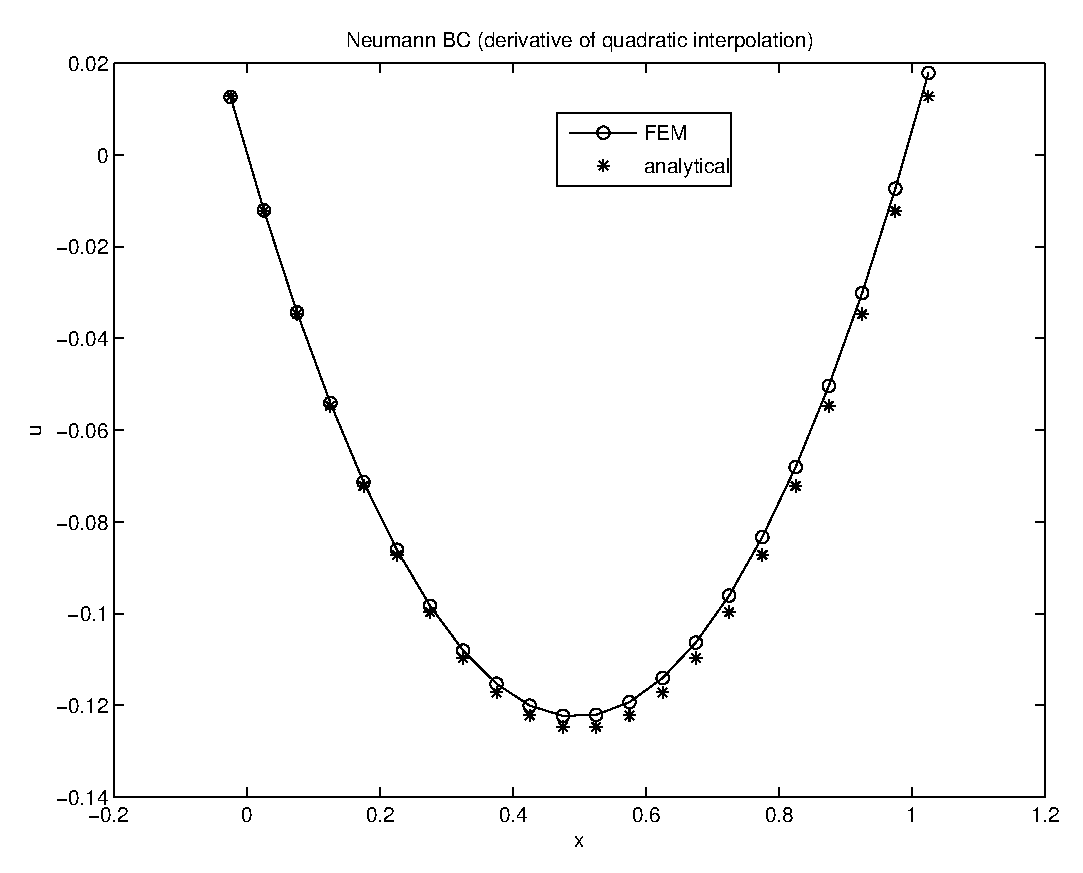
\includegraphics{neumannquad.eps}}\\
\caption{Neumann Boundary Conditions on End of Domain (Solution of Finite Element Method With Quadratic Interpolation of Boundary Conditions).}\label{fig:neumannQuad}
\end{figurehere}
\end{center}
We want to look carefully at the number of digits exactly satisfied by this comparison.
\footnote{The finite element solutions do converge to the analytical solution that can be obtained easily to the problem we are solving. Convergence is obtained with decreasing the mesh size. For the specific coefficients we are choosing, and for the pure Dirichlet boundary conditions, the analytical solution reads $u = \frac{x^2}{2}$. For the Neumann boundary condition case, the analytical solution reads for the specific coefficients we chose above $u = \frac{x^2}{2} -\frac{1}{2}x$.}
\subsection{Derivative of Linear Interpolation: Bug in analytical solution}
Using the linear interpolation for the Dirichlet boundary condition on the cut cell edge, the Neumann boundary condition can be expressed as follows:
\begin{equation}
 \frac{\partial u}{\partial x}\vert_L = \frac{\partial N_{n-1}}{\partial x}u_{n-1}+\frac{\partial N_n}{\partial x}u_n,
\end{equation}
where
\begin{eqnarray}
\frac{\partial N_{n-1}}{\partial x} &=& \frac{-1}{\Delta x},\\
\frac{\partial N_n}{\partial x} &=&  \frac{1}{\Delta x}.
\end{eqnarray}
For the specific problem we are looking at, the solution is depicted in figure \ref{fig:neumannLinear}.
\begin{center}
\begin{figurehere} 
\scalebox{0.7}{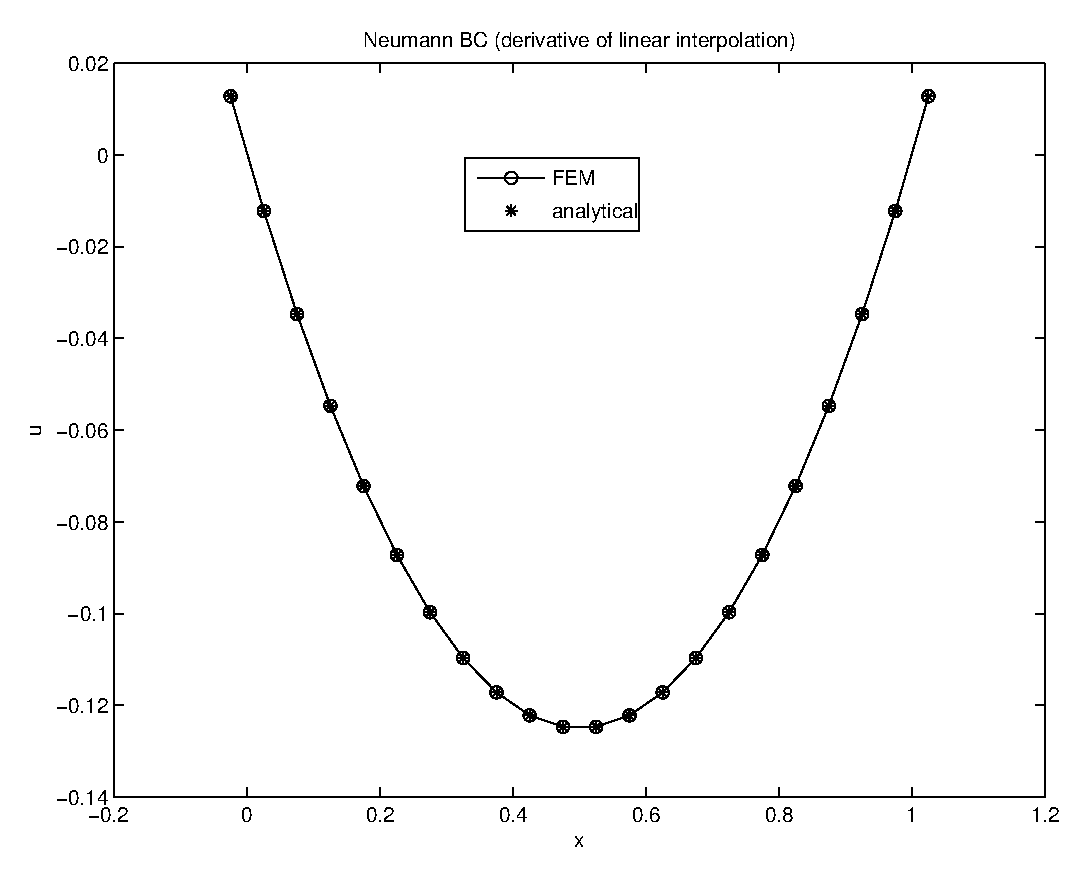
\includegraphics{neumannlinear.eps}}\\
\caption{Neumann Boundary Conditions on End of Domain (Solution of Finite Element Method With Linear Interpolation of Boundary Conditions).}\label{fig:neumannLinear}
\end{figurehere}
\end{center}
Figure \ref{fig:neumannLinear} shows that the linear interpolation (constant imposition of the Neumann boundary conditions) hits the analytical solution exactly. We want to look carefully at the number of digits exactly satisfied by this comparison.
The analytical solution at the unknowns' positions reads:
\begin{verbatim}
u_nE =

   0.012812500000000
  -0.012187500000000
  -0.034687500000000
  -0.054687500000000
  -0.072187500000000
  -0.087187500000000
  -0.099687500000000
  -0.109687500000000
  -0.117187500000000
  -0.122187500000000
  -0.124687500000000
  -0.124687500000000
  -0.122187500000000
  -0.117187500000000
  -0.109687500000000
  -0.099687500000000
  -0.087187500000000
  -0.072187500000000
  -0.054687500000000
  -0.034687500000000
  -0.012187500000000
   0.012812500000000
\end{verbatim}
The finite element solution at the unknowns' positions reads:
\begin{verbatim}
u_n =

   0.012812500000000
  -0.012187500000000
  -0.034687500000000
  -0.054687500000000
  -0.072187500000000
  -0.087187500000000
  -0.099687500000000
  -0.109687500000000
  -0.117187500000000
  -0.122187500000000
  -0.124687500000000
  -0.124687500000000
  -0.122187500000000
  -0.117187500000000
  -0.109687500000001
  -0.099687500000001
  -0.087187500000001
  -0.072187500000001
  -0.054687500000001
  -0.034687500000001
  -0.012187500000001
   0.012812499999999
\end{verbatim}
We do not notice any distinction between the two solutions to double precision accuracy.
\subsection{Corrected: Derivative of Linear Interpolation and Quadratic Interpolation}
Basically, the implementation of the linear and quadratic interpolations are bug-free. The Neumann boundary conditions have been imposed correctly in the finite element solution. However, the comparison with the analytical solution has not be done correctly. The analytical solution has accounted for a certain placement of the Neumann boundary condition, that is $\overline{\frac{\partial u}{\partial x}}\vert_L=0.5$. This has been mistakenly given in the problem definition. Changing the value of $\alpha$ changes the end of the physical domain, and therefore the position of the Neumann boundary condition. We change the definition of the problem to the following:
\begin{eqnarray}
L = 1, \hspace{0.5cm}, h = 0.05, \hspace{0.5cm}A= 3, \hspace{0.5cm}\overline{u}\vert_0 = 0.0,\\ 
\overline{\frac{\partial u}{\partial x}}\vert_{L_{c}}=0.5, \hspace{0.5cm}K = -3,\hspace{0.5cm}\alpha = 0.9, L_{c} = L + h (\alpha - 1) = 0.995.
\end{eqnarray}
Thus, the analytical solution for this specific case reads:
\begin{eqnarray}
 u = \frac{x^2}{2} + 0.5 - L_{c},\\
u = \frac{x^2}{2} -0.495.
\end{eqnarray}
Once $L_{c}$ changes, so do both the analytical solution and the finite element solution.
\subsubsection{Derivative of Linear Interpolation}
The finite element solution at the unknowns' positions reads:
\begin{verbatim}
u_n =

   0.012812500000000
  -0.012187500000000
  -0.034687500000000
  -0.054687500000000
  -0.072187500000000
  -0.087187500000000
  -0.099687500000000
  -0.109687500000000
  -0.117187500000000
  -0.122187500000000
  -0.124687500000000
  -0.124687500000000
  -0.122187500000000
  -0.117187500000000
  -0.109687500000001
  -0.099687500000001
  -0.087187500000001
  -0.072187500000001
  -0.054687500000001
  -0.034687500000001
  -0.012187500000001
   0.012812499999999
\end{verbatim}
The analytical solution at the unknowns' positions reads:
\begin{verbatim}
u_nE =

   0.012687500000000
  -0.012062500000000
  -0.034312500000000
  -0.054062500000000
  -0.071312500000000
  -0.086062500000000
  -0.098312500000000
  -0.108062500000000
  -0.115312500000000
  -0.120062500000000
  -0.122312500000000
  -0.122062500000000
  -0.119312500000000
  -0.114062500000000
  -0.106312500000000
  -0.096062500000000
  -0.083312500000000
  -0.068062500000000
  -0.050312500000000
  -0.030062500000000
  -0.007312500000000
   0.017937500000000
\end{verbatim}
We do not notice a deviation between the two solutions beginning from the third after comma digit (see also figure \ref{fig:neumannQuad2}).
\begin{center}
\begin{figurehere} 
\scalebox{0.7}{\includegraphics{neumannquad2.eps}}\\
\caption{Neumann Boundary Conditions on End of Domain (Solution of Finite Element Method With Quadratic Interpolation of Boundary Conditions).}\label{fig:neumannQuad2}
\end{figurehere}
\end{center}
\subsubsection{Derivative of Quadratic Interpolation}
The finite element solution at the unknowns' positions reads:
\begin{verbatim}
u_n =

   0.012687500000000
  -0.012062500000000
  -0.034312500000000
  -0.054062500000000
  -0.071312500000000
  -0.086062500000000
  -0.098312500000000
  -0.108062500000001
  -0.115312500000001
  -0.120062500000001
  -0.122312500000001
  -0.122062500000001
  -0.119312500000001
  -0.114062500000001
  -0.106312500000002
  -0.096062500000002
  -0.083312500000002
  -0.068062500000002
  -0.050312500000002
  -0.030062500000002
  -0.007312500000002
   0.017937499999998
\end{verbatim}
The analytical solution at the unknowns' positions reads:
\begin{verbatim}
u_nE =

   0.012687500000000
  -0.012062500000000
  -0.034312500000000
  -0.054062500000000
  -0.071312500000000
  -0.086062500000000
  -0.098312500000000
  -0.108062500000000
  -0.115312500000000
  -0.120062500000000
  -0.122312500000000
  -0.122062500000000
  -0.119312500000000
  -0.114062500000000
  -0.106312500000000
  -0.096062500000000
  -0.083312500000000
  -0.068062500000000
  -0.050312500000000
  -0.030062500000000
  -0.007312500000000
   0.017937500000000
\end{verbatim}
We do notice a deviation between the two solutions starting from the third after comma digit (see also figure \ref{fig:neumannLin2}).
\begin{center}
\begin{figurehere} 
\scalebox{0.7}{\includegraphics{neumannlin2.eps}}\\
\caption{Neumann Boundary Conditions on End of Domain (Solution of Finite Element Method With Linear Interpolation of Boundary Conditions).}\label{fig:neumannLin2}
\end{figurehere}
\end{center}
\subsubsection{Interpretations}
The results obtained in the previous two sections is consistent for different values of $\alpha$. The result, the derivative of a quadratic interpolation is more accurate than the derivative of a linear interpolation to impose the flux, we obtained does have an explanation. The analytical solution is quadratic. Therefore, the flux is a linear function. When we do impose a quadratic displacement interpolation, and thus a linear flux interpolation on the boundary, we do obtain quadratic convergence. In the case, where we use a linear interpolation of the displacement, and thus a constant flux function, we do not obtain convergence. The conclusion is that we have to remain consistent with the degree of the answer (linear, quadratic, cubic etc) when we impose the boundary conditions by interpolation in order to obtain convergence.
\subsection{Finite Element Flux Solution}
We know that the fluxes obtained from the finite element solution are discontinuous at the element boundaries.\\
The flux in an element is given by:
\begin{equation}
 \frac{\partial u}{\partial x} = \sum_{I}\frac{\partial N_I}{\partial x}\frac{\partial \xi}{\partial x}u_I,
\end{equation}
where the index $I$ stands for the nodal index.
The problem we have solved in the previous section results into a quadratic displacement solution, and therefore into a linear flux function. The flux solution are depicted in the figures for both Neumann boundary condition approaches.
\begin{center}
\begin{figurehere} 
\scalebox{0.7}{\includegraphics{fluxquad.eps}}\\
\caption{Flux Solution (Solution of Finite Element Method With Quadratic Interpolation of Boundary Conditions).}\label{fig:fluxquad}
\end{figurehere} 
\end{center}
\begin{center}
\begin{figurehere} 
\scalebox{0.7}{\includegraphics{fluxlin.eps}}\\
\caption{Flux Solution (Solution of Finite Element Method With Linear Interpolation of Boundary Conditions).}\label{fig:fluxlin}
\end{figurehere}
\end{center}
We note here that both approaches are simply an approximation to the anallytical solution. This behavior was not expected, since the quadratic interpolation of the Neumann boundary condition did deliver the exact solution. Therefore, one expects that its derivative would also be exact. \\
It is to remember that we are comparing the analytical solution with the finite element solution at sampling points, i.e. the nodes. We know that on many occasions the displacements, are most accurately sampled at the nodes and that the gradients are best sampled at some interior points \cite{TaylorZienkiewicz}. The solution at the appropriate sampling points exhibit superconvergence according to the Herrmann theorem and show an error which decreases more rapidly than elsewhere.\\
While solving our problem, we do notice that nodes are the appropriate sampling points to obtain superconvergence. This happens to be the case because the weighting function used here contain the exact solution and because of the use of linear elements (solution at inner nodes of higher order elements tend to deviate from the exact solution and distortion is more likely to happen). \\
However, the nodes do not seem to be the best sampling points of the finite element flux solution and therefore should be sampled elsewhere in the interior of the elements. It can be shown that sampling somewhere near the center of each element is needed. The center of the element hits here the position of the gauss point needed to exactly integrate the analytical flux solution. We remember here that the flux solution is linear. Therefore, one gauss point is enough to accurately integrate the flux solution over one element. At the gauss points, the flux is expected to be exact.\\
Using these information, we do compare the analytical and finite element fluxes at the element centers. The solutions are depicted in figures \ref{fig:fluxquadCenter}
and \ref{fig:fluxlinCenter} .
\begin{center}
\begin{figurehere} 
\scalebox{0.7}{\includegraphics{neumannQuadCenter.eps}}\\
\caption{Flux Solution (Solution of Finite Element Method With Quadratic Interpolation of Boundary Conditions).}\label{fig:fluxquadCenter}
\end{figurehere} 
\end{center}
\begin{center}
\begin{figurehere} 
\scalebox{0.7}{\includegraphics{neumannLinCenter.eps}}\\
\caption{Flux Solution (Solution of Finite Element Method With Linear Interpolation of Boundary Conditions).}\label{fig:fluxlinCenter}
\end{figurehere}
\end{center}
The analytical flux at the center points is given by:
\begin{verbatim}
 du_nE =

  -0.455000000000000
  -0.405000000000000
  -0.355000000000000
  -0.305000000000000
  -0.255000000000000
  -0.205000000000000
  -0.155000000000000
  -0.105000000000000
  -0.055000000000000
  -0.005000000000000
   0.045000000000000
   0.095000000000000
   0.145000000000000
   0.195000000000000
   0.245000000000000
   0.295000000000000
   0.345000000000000
   0.395000000000000
   0.445000000000000
   0.495000000000000
   0.545000000000000
   0.595000000000000
\end{verbatim}
The finite element flux at the center point for the quadratic interpolation approach reads:
\begin{verbatim}
 du_n =

  -0.455000000000001
  -0.405000000000001
  -0.355000000000001
  -0.305000000000001
  -0.255000000000001
  -0.205000000000001
  -0.155000000000001
  -0.105000000000001
  -0.055000000000001
  -0.005000000000002
   0.044999999999999
   0.094999999999998
   0.144999999999999
   0.194999999999999
   0.244999999999999
   0.294999999999999
   0.344999999999999
   0.394999999999998
   0.444999999999998
   0.494999999999999
   0.545000000000000
   0.545000000000000
\end{verbatim}
The finite element flux at the center point for the linear interpolation approach reads:
\begin{verbatim}
 du_n =

  -0.500000000000001
  -0.450000000000001
  -0.400000000000001
  -0.350000000000001
  -0.300000000000001
  -0.250000000000001
  -0.200000000000001
  -0.150000000000001
  -0.100000000000001
  -0.050000000000001
  -0.000000000000001
   0.049999999999999
   0.099999999999999
   0.149999999999999
   0.199999999999999
   0.249999999999999
   0.300000000000000
   0.349999999999999
   0.399999999999998
   0.449999999999999
   0.500000000000001
   0.500000000000001
\end{verbatim}
The new sampling confirms that the quadratic interpolation of the solution, i.e. the linear interpolation of the flux leads to accurate results.
\section{Two-Dimensional Approach}
\subsection{Canonical Problem: Circular Physical Domain}\label{sec:canonicalPr}
We want to solve the following problem using the finite element method on a rectangular two dimensional grid:
\begin{eqnarray}
 A \bigtriangleup u + f &=& 0,\\
 A \bigtriangledown.(\bigtriangledown u) + f &=& 0,
\end{eqnarray}
where $A$ is a material constant and f a weighting constant function.\\
Note here that only the geometry is two-dimensional. The function we are solving for is scalar (not vectorial), i.e. the nodes do have one single degree of freedom.\\
Since the problem is two-dimensional, the function $u$ does not change on the third dimension, and we can omit this dependence.
\subsection{Analytical Solution}\label{sec:analsol}
We can express our unknown $u$ in terms of polar coordinates ($r$, $\theta$). Since the geometry is axisymmetric, the function $u$ does not depend on the angular direction but on the radial position. 
\begin{eqnarray}
 A \bigtriangledown.(\bigtriangledown u) + f &=& 0,\\
 A (\frac{\partial^2 u}{\partial r^2} + \frac{1}{r}\frac{\partial u}{\partial r} + \frac{1}{r^2}\underbrace{\frac{\partial ^2u}{\partial \theta^2}}_{=0} + \underbrace{\frac{\partial ^2 f}{\partial z^2}}_{=0}) + f &=& 0,\\
 A (\frac{\intd^2 u}{\intd r^2} + \frac{1}{r}\frac{\intd u}{\intd r}) + f &=& 0,\\
 \frac{\intd^2 u}{\intd r^2} + \frac{1}{r}\frac{\intd u}{\intd r} &=& -\frac{f}{A}.\\
\end{eqnarray}
The homogeneous solution to the last equation is given by:\
\begin{eqnarray}
 \text{Let } v =  \frac{\intd u}{\intd r},\\
 \text{The equation reads then: }\frac{\intd v}{\intd r}+\frac{1}{r}v = 0,\\
 \frac{\intd v}{v} = -\frac{\intd r}{r},\\
\int \frac{\intd v}{ v} = \int -\frac{\intd r}{r} + \widetilde{C},\\
\text{ln}(v) = - \text{ln}(r) + \widetilde{C},\\
\text{ln}(v) = \text{ln}(\frac{1}{r}) + \widetilde{C},\\
\text{e}^{\text{ln}(v) } = \text{e}^{\text{ln}(\frac{1}{r}) + \widetilde{C}},\\
v = \text{e}^{\text{ln}(\frac{1}{r})}\underbrace{\text{e}^{\widetilde{C}}}_{C_1},\\
v = C_1\frac{1}{r},\\
\frac{\intd u}{\intd r} = \frac{C_1}{r},\\
\int \intd u =  C_1 \int \frac{\intd r}{r},\\
u = C_1 \text{ln}(r) + C_2.\\ 
\end{eqnarray}
Since a solution has to exist at the center of the circle, where $r = 0$, the term $\text{ln}(r)$ blows up as it approaches the center. We omit this term by setting $C_1 = 0$. Thus, the homogeneous solution reads:
\begin{equation}
u_h = C_2.
\end{equation}
We now have to solve for the particular solution from:
\begin{equation}
 \frac{\intd^2 u}{\intd r^2} + \frac{1}{r}\frac{\intd u}{\intd r} = -\frac{f}{A}.
\end{equation}
One assumes that the particular solution is of the form:
\begin{equation}
 u = \frac{f}{A}(ar^2 + br),
\end{equation}
where $a$ and $b$ are constants that have to be determined. 
Using this assumption, we obtain:
\begin{eqnarray}
 \frac{\intd^2 u}{\intd r^2} + \frac{1}{r}\frac{\intd u}{\intd r} = -\frac{f}{A},\\
\frac{f}{A}(2a)+ \frac{1}{r}\frac{f}{A}(2ar + b)= -\frac{f}{A},\\
2a  + \frac{1}{r}(2ar + b)= -1,\\
4a  + \frac{1}{r} b= -1.
\end{eqnarray}
In order to obtain an acceptable solution at the center of the circle, we set $b = 0$. Finally, the particular solution reads:
\begin{eqnarray}
4a = -1,\\
a = -\frac{1}{4},\\
u_p = -\frac{f}{4A}r^2.
\end{eqnarray}
The total solution reads:
\begin{equation}
 u = u_h + u_p = C_2 - \frac{f}{4A}r^2.
\end{equation}
Given the Dirichlet boundary condition, where $u = \overline{u}$ at the boundary of the circular physical domain. Let's denote $R$ to be the radius of the circle. Therefore, $u = \overline{u}$  for $r = R$. 
\begin{eqnarray}
 \overline{u} = C_2 - \frac{f}{4A}R^2,\\
C_2 = \overline{u} + \frac{f}{4A}R^2,\\
u = \overline{u} + \frac{f}{4A}R^2 - \frac{f}{4A}r^2.
\end{eqnarray}
In the end, we realize that the solution is a combination of one-dimensional solutions since the solution varies only on each ray in the circle, and the solutions on the rays are independent of each other. 
\subsection{Weak Form}
The weak form of the problem can be derived as follows:
\begin{eqnarray}
\int_{\Omega}(A \bigtriangledown.(\bigtriangledown u )  + f) v  \intd \Omega = 0,\\
\int_{\Omega}A \bigtriangledown.(\bigtriangledown u) v + fv \intd \Omega = 0,\\
\int_{\Omega}A \bigtriangledown.((\bigtriangledown u )v) -A \bigtriangledown u\cdot\bigtriangledown v  + fv \intd \Omega = 0,\\
\int_{\Omega}A \bigtriangledown.((\bigtriangledown u) v) \intd\Omega -A\int_{\Omega} \bigtriangledown u\cdot\bigtriangledown v  + fv \intd \Omega = 0,\\
\int_{\partial\Omega}A ((\bigtriangledown u)v) \mb{n}\intd(\partial\Omega) -A\int_{\Omega} \bigtriangledown u\cdot\bigtriangledown v  + fv\intd \Omega = 0,\\
\int_{\partial\Omega}A ((\bigtriangledown u)v) \mb{n}\intd(\partial\Omega) + fv \intd \Omega = A\int_{\Omega} \bigtriangledown u\cdot\bigtriangledown v\intd \Omega.\\
\end{eqnarray}
The function $u$ is imposed to pure Dirichlet conditions, s.t.:
\begin{eqnarray}
 u&=& \overline{u} \hspace{0.5cm}\text{on} \hspace{0.5cm}\partial\Omega_u,\\
\end{eqnarray}
Therefore, the weak form simplifies to:
\begin{equation}
\int_{\partial\Omega} fv \intd \Omega = A\int_{\Omega} \bigtriangledown u\cdot\bigtriangledown v\intd \Omega.
\end{equation}
\subsection{Discretization}
The following discretization convention has been used to create the vector-matrix entries:
\begin{eqnarray}
\widehat{\Phi}_1 &=& \frac{1}{4}(1 -\xi)(1 - \eta),\\
\widehat{\Phi}_2 &=& \frac{1}{4}(1 + \xi)(1 - \eta),\\
\widehat{\Phi}_3 &=& \frac{1}{4}(1 + \xi)(1 + \eta),\\
\widehat{\Phi}_4 &=& \frac{1}{4}(1 - \xi)(1  + \eta),\\
\widehat{\Phi}^e &=& \left( \begin{array}{cc}
\widehat{\Phi}^e_1 \\
\widehat{\Phi}^e_2 \\
\widehat{\Phi}^e_3 \\
\widehat{\Phi}^e_4
\end{array} \right),\\
D \widehat{\Phi}^e &=& \left( \begin{array}{cc}
\frac{\partial \widehat{\Phi}^e_1}{\partial \xi}& \frac{\partial \widehat{\Phi}^e_1}{\partial \eta} \\
\frac{\partial \widehat{\Phi}^e_2}{\partial \xi}& \frac{\partial \widehat{\Phi}^e_2}{\partial \eta} \\
\frac{\partial \widehat{\Phi}^e_3}{\partial \xi}& \frac{\partial \widehat{\Phi}^e_3}{\partial \eta} \\
\frac{\partial \widehat{\Phi}^e_4}{\partial \xi}& \frac{\partial \widehat{\Phi}^e_4}{\partial \eta}
\end{array} \right),\\
X^e &=& \left( \begin{array}{cccc}
x_1& x_2 & x_3 & x_4 \\
y_1& y_2 & y_3 & y_4 
\end{array} \right),\\
F &=& (X^e)D\widehat{\Phi}^e,\\
C &=& F^TF,\\
J &=& det(F).
\end{eqnarray}
Therefore, we obtain:
\begin{eqnarray}
K_{ij}^e = \int_{\Omega^e_0}AD\widehat{\Phi}^eC^{-1}(D\widehat{\Phi}^{e})^TJ\intd \Omega,\\
R_i^e = \int_{\Omega^e_0}f\widehat{\Phi}^eJ\intd \Omega 
\end{eqnarray}
% \begin{eqnarray}
% \mb{u} &=& \mb{N}\widehat{\mb{u}},\\
% \mb{N} &=& \left[ \begin{array}{cccccccc}
% N_1 & 0 & N_2 & 0 & N_3 & 0 & N_4 & 0 \\
% 0 & N_1 & 0 & N_2 & 0 & N_3 & 0 & N_4\end{array} \right]\\
% \bigtriangledown \mb{u} &=& \mb{B}\widehat{\mb{u}},\\
% \mb{B} &=& \left[ \begin{array}{cccccccc}
% N_{1,1} & 0 & N_{2,1} & 0 & N_{3,1} & 0 & N_{4,1} & 0 \\
% 0 & N_{1,2} & 0 & N_{2,2} & 0 & N_{3,2} & 0 & N_{4,2}\\
% N_{1,2} & 0 & N_{2,2} & 0 & N_{3,2} & 0 & N_{4,2} & 0 \\
% 0 & N_{1,1} & 0 & N_{2,1} & 0 & N_{3,1} & 0 & N_{4,1}\\\end{array} \right]
% \end{eqnarray}
\subsection{Geometry}
The geometry chosen for the canonical problem is a circle with defined center position and radius that is discretized using a rectangular grid (Figure \ref{fig:geometry}).
\begin{center}
\begin{figurehere} 
\scalebox{0.7}{\includegraphics{geometry.eps}}\\
\caption{Circular Physical Domain and Cartersian Grid}\label{fig:geometry}
\end{figurehere}
\end{center}

\newpage
\subsection{Solution Method}\label{sec:algorithm}
The elements of the rectangular grid are sorted into three categories: fully covered by the physical domain, partially covered by the physical domain and totally outside of the physical domain (see figure \ref{fig:elementtypes}).\\ We are interested in the first two categories. The treatment of the first category of elements is straightforward and is done in the usual manner. 
\begin{center}
\begin{figurehere} 
\scalebox{0.7}{\includegraphics{elementtypes.eps}}\\
\caption{$3$ Types of elements: partial (green), full (blue), outside of domain (red)}\label{fig:elementtypes}
\end{figurehere}
\end{center}
The partial elements are subject to boundary conditions. In addition, it has to be determined which nodes of the partial elements do lie inside, outside or on the boundary of the domain. The nodes that do lie outside of the domain do no have a material stiffness and therefore have to be treated differently.\\ 
Without consideration of the boundary conditions and the hanging nodes of the partial elements, the element stiffness matrices and the element force vectors are generated and assembled for full and partial elements. After assembling, the entries associated with the outside of the domain elements remain zero and have to be taken care of in order to solve the system of equations. \\
The rows of the system associated with the hanging nodes do contain contribution from the system stiffness which is physicall not consistent. However, the hanging nodes are subject to a deformation due to the deformation of the inner nodes as well as the boundary conditions. Therefore, and in analogy to the onedimensional study done before, the row associated with the hanging nodes is substituted by a boundary condition interpolation equation. In order to do this modification, the intersection of the physical domain with the rectangular element has to be determined. The intersection points could be the hanging nodes themselves, but this is just one special case. The intuition is to interpolate the intersection point condition in terms of the unknowns of the nodes (the unknowns are here scalars). It is optimal to have as many intersection points as hanging nodes or at least more intersection points that hanging nodes. Each intersection point interpolation substitutes an equation in the stiffness matrix. Now, we have to be careful and not substitute the equations randomly. We want at the end to have a non-singular matrix, i.e. zero diagonal entries are not allowed. One has to figure out the appropriate intersection point to choose for an interpolation condition. If the hanging node happens to be an intersection point itself, then we are done. The criteria of having non-zero diagonal elements is a difficult criteria to fulfill once the problems get harder.  Therefore, an idea is to take an intersection point lying on one of the edges for which the hanging node is a corner node. This works perfectly smooth assuming correct implementation and treatment of round-off errors.\\
Now, one has to think of the hanging nodes that either do not coincide with an intersection point and do not have a neighboring intersection point. One can treat this special case by creating ``fake'' intersection points. These points do lie on the boundary of the physical domain but do not lie on any of the edges of the element. These elements can be created by averaging two intersection points. Averaging might be the wrong word for it, because the average of two intersection points might not lie on the physical domain boundary. Therefore, averaging can happen in one direction (horizontal or vertical) and the associated other coordinate can be determined from the geometric equation of the physical domain. Obviously, the ``fake'' intersection point does lie inside of the element domain. The interpolation equation does create a diagonal entry.\\
Some representatives of these cases are depicted in figure \ref{fig:partialelements}.
\begin{center}
\begin{figurehere} 
\scalebox{0.7}{\input{partialelementcases.pstex_t}}\\
\caption{Partial Element Cases: (a) $3$ hanging nodes and $2$ intersection points (creation of a ``fake'' intersection point is necessary) (b) $2$ hanging nodes and $2$ intersection points (c) $2$ hanging nodes and two intersection points (one of them is a hanging node) (d) $3$ hanging nodes and $2$ intersection points (that are $2$ hanging nodes)}\label{fig:partialelements}
\end{figurehere}
\end{center}

The stiffness matrix might still contain zero diagonal entries that are associated with nodes coming from elements that do totally lie outside of the domain. One can assume that these nodes do not deform at all. Therfore, the rows and columns  containing zero diagonal entries can simply be deleted. From the implementation point of view, an efficient and flexible data storage structure is needed here. \\
A simplifying assumption has been made here, that an element that lies totally outside of the physical domain except that one node does lie on the boundary, can be treated as being outside of the domain. The ``three'' hanging nodes are not supposed to deform. The node lying on the boundary will be treated since it belongs to at least one partial element. 
\begin{center}
\begin{figurehere} 
\scalebox{0.7}{\includegraphics{specialcase.eps}}\\
\caption{Special Case of Elements Outside of Domain}\label{fig:specialcase}
\end{figurehere}
\end{center}
Just for the sake of completeness, one other special case needs to be handled when the rectangular grid is only covered by a single element. One does take the simple case, where the physical domain is a rectangle, but free shaped. Hence, the element is partially covered by the physical domain and all of the element nodes are hanging nodes (see figure \ref{fig:oneelement}). If one does not pay attention, the above discussed algorithm will analyze the element as being outside of the domain since all nodes lie outside of the domain. Therefore, a case catch must be implemented. If the physical domain does not touch the edges of the element, there is no way to solve this problem. But, also if the $4$ intersection points do exist and if it is symmetric as shown in figure \ref{fig:oneelement}, the interpolation equations will create a rank $0$ system that is unsolvable. But, seriously, we do not expect an accuracy from solving a complicated finite element problem using a single element. Therefore, one might just want to omit this case and consider solving this problem using let's say a minimum of $4$ elements.
\begin{center}
\begin{figurehere} 
\scalebox{0.7}{\includegraphics{onelement.eps}}\\
\caption{One Element Rectangular Grid}\label{fig:oneelement}
\end{figurehere}
\end{center}
\subsection{Convergence Study: First Attempt}\label{sec:erroranalysis}
We want to study and understand the convergence of this new algorithm. We solve the following problem: 
\begin{eqnarray}
A \bigtriangleup u + f &=& 0,\\
A &=& 1, \hspace{0.5cm} f = 1,\\
u &=& \overline{u} = 0.0 \hspace{0.5cm} \text{on the entire boundary}.
\end{eqnarray}
For different rectangular grid element sizes, the error that is made by this algorithm to the interior node values is determined as follows:
\begin{eqnarray}\label{eqn:H0norm}
\Vert e \Vert &=& \frac{\Vert \mb{u}_n^i - \mb{u}^i \Vert_{\infty}}{n},\\
 &=& \frac{ \sum_j  \vert \mb{u}_{n_{j}}^i - \mb{u}_j^i \vert}{n},
\end{eqnarray}
where $n$ is the total number of the interior nodes to the physical domain, $\mb{u}_n^i$ is the algorithm solution at the interior nodes and $\mb{u}^i$ is the analytical solution at the nodes. The analytical solution has been derived in section \ref{sec:analsol}.
The error as a function of the total number of interior nodes is depicted in the log-log-plot in figure \ref{fig:convergence}. One notices the consistent linear convergence of the algorithm, i.e. the error is of the order of the element size. One does expect this behavior because of the non-propagation of the boundary information to the neighboring elements. The method imposed the boundary condition at the hanging nodes using an interpolation equation in the domain of one element. We suspect that the expansion of the interpolation domain will effect the convergence behavior positively.
\begin{center}
\begin{figurehere} 
\scalebox{0.7}{\includegraphics{convergence.eps}}\\
\caption{Convergence Study}\label{fig:convergence}
\end{figurehere}
\end{center}
The test results are tabulated in the table \ref{tab:convergence}:
\begin{center}
\begin{tablehere}
\begin{tabular}{cc}
 $\Vert e \Vert$ & n \\
\hline
\hline
0.022613849221600 & 5 \\
0.012440258770754 & 13 \\
0.003636812889227 & 49\\
7.512968349467671e-04 & 197\\
2.211819084109193e-04 &  797\\
4.266346728977254e-05 & 3209\\
1.173832783656672e-05 & 12853\\
3.024078476989026e-06 & 51433\\
\end{tabular}
\caption{Convergence Test Results}\label{tab:convergence}
\end{tablehere}
\end{center}
There is a small undesirable kink in the middle of the convergence curve. We correct this by doing an additional test. The corrected convergence behavior is depicted in figure \ref{fig:convergence2} and the additional test results are given in table \ref{tab:convergenceAdd}.
\begin{center}
\begin{tablehere}
\begin{tabular}{cc}
 $\Vert e \Vert$ & n \\
\hline
\hline
1.527300058654243e-04 & 848\\
1.160100600789700e-04 & 1257
\end{tabular}
\caption{Additional Convergence Test Results}\label{tab:convergenceAdd}
\end{tablehere}
\end{center}
\begin{center}
\begin{figurehere}
\scalebox{0.7}{\includegraphics{convergence2.eps}}\\
\caption{Corrected Convergence Study}\label{fig:convergence2}
\end{figurehere}
\end{center}
As we see, the curve is not really straight.  Actually, when we further refine the mesh, the curve loses linearity and drops vertically to a smaller error. One wonders about the reasons of this behavior. A thought would be that elements with very small physical coverage ratio are present and affect the presented algorithm.
A second look at the convergence behavior made us rethink about out statement. The H$0$ error norm we are introducing in equation (\ref{eqn:H0norm}) should be quadratic in h, i.e. the slope in the log-log plot of the error as a function of the number of interior nodes should be of order $2$. The choice of the number of the interior node as the independent variables turns out to be a bad choice. In the following sections, we will see that the independent variable should be better the element size.\\
The more we look at the numerical solution and the analytical solution and compare them, we doubt on the convergence conclusions we made above. The two solutions are depicted in the figures \ref{fig:anacirc} and \ref{fig:numcirc}.
\begin{center}
\begin{figurehere}
\scalebox{0.7}{\includegraphics{analyticalsolutioncircular128e.eps}}\\
\caption{Analytical Solution for Circular Domain}\label{fig:anacirc}
\end{figurehere}
\end{center}
\begin{center}
\begin{figurehere}
\centering
\scalebox{0.7}{\includegraphics{femsolutioncircular128e.eps}}\\
\caption{Numerical Solution for Circular Domain}\label{fig:numcirc}
\end{figurehere}
\end{center}

\subsection{Comparison to the One-Dimensional Algorithm}
We want to verify the convergence behavior of the two dimensional algorithm by comparing it to the convergence behavior of the one-dimensional problem. We studied the one-dimensional problem carefully, and we were able to make consistent conclusions.\\
We will solve the one-dimensional problem given in (\ref{eqn:problem}) for different mesh sizes, with the following parameters:
\begin{eqnarray}
\overline{u}\vert_{0} = 0.0,\hspace{0.5cm} \overline{u}\vert_{L_c} = 0.5, \hspace{0.5cm} K = -1\\
A = 1, \hspace{0.5cm}, L_c = 1,\hspace{0.5cm}L_0 = 0,
\end{eqnarray}
where $L_0$ and $L_c$ are the left and right coordinates of the one-dimensional physical domain.\\
We follow the error analysis and definition presented in section \ref{sec:erroranalysis}.
Using a linear interpolation, i.e no coupling between the elements, the test results are tabulated in the table \ref{tab:linear1d} and depicted in the log-log-plot \ref{fig:lin1d}:
\begin{center}
\begin{tablehere}
\begin{tabular}{cc}
 $\Vert e \Vert$ & n \\
\hline
\hline
0.031250000000000 & 2\\
0.007812500000000 & 4\\
0.001953125000000 & 8\\
4.882812500000000e-04 & 16\\
1.220703125001110e-04 & 32\\
3.051757812500000e-05 & 64\\
7.629394531250000e-06 & 128\\
1.907348632701478e-06 & 256\\
4.768371582031250e-07 & 512\\
1.192092895507812e-07 & 1024\\
2.980232238769531e-08 & 2048\\
7.450580596923828e-09 & 4096\\
\end{tabular}
\caption{Convergence Test Results of One-dimensional Case Without Coupling}\label{tab:linear1d}
\end{tablehere}
\end{center}
\begin{figurehere}[ht]
\centering
\scalebox{0.7}{\includegraphics{linear1d.eps}}\\
\caption{Convergence Study of One-dimensional Case Without Coupling}\label{fig:lin1d}
\end{figurehere}
The results obtained show quadratic convergence that does not confirm the results obtained from the two-dimensional counter-example. The error is calculated at the nodes that are considered to be superconvergent, hence the quadratic convergence. Therefore, something is wrong with the error analysis for the two-dimensional case.\\
For the one-dimensional case, if we propagate the interpolation information to a neighbor element, i.e. if we couple the two first and the two last elements, the one-dimensional study does lead to an interesting effect. An error of the order of the machine epsilon is made, when one would use only two elements. I.e. the coupling hits the exact solution for the coarsest possible element size. Decreasing the mesh size leads to an increase in the error, even though the numerical solution does match the analytical one (Results are tabulated in table \ref{tab:quadratic1d}). We suspect that the round-off errors overwhelm the numerical error. Since the numerical error is tiny small, if not vanishing for the problem we are solving, the round-off error dominates and leads to an increase in the total error instead of a decrease.\\
\begin{center}
\begin{tablehere}
\begin{tabular}{cc}
 $\Vert e \Vert$ & n \\
\hline
\hline
4.163336342344337e-17 & 2\\
1.296705798292663e-16 & 4 \\
1.112825109839122e-15 & 8 \\
2.465150479580291e-15 & 16\\
2.081267016368349e-14 & 32 \\
4.223409274216328e-14 & 64 \\
3.404037170412835e-13 & 128\\
6.676058021833596e-13 & 256\\
5.472485393445345e-12 & 512\\
1.088767981445528e-11 & 1024\\
8.732092397230042e-11 & 2048\\
1.748866421536470e-10 & 4096\\
1.396787000525363e-09 & 8192
\end{tabular}
\caption{Convergence Test Results With Coupling}\label{tab:quadratic1d}
\end{tablehere}
\end{center}
If we look at the numerical solution $u_n$ and compare it to the analytical solution $u$ for different element sizes, we deduce that the roundoff error is overwhelming the truncation error. The algorithm hits the analytical solution almost exactly and due to the nature of the problem (linear) but the numerical noise leads to an increase in the error. See tables \ref{tab:linear1dcoupl1}, \ref{tab:linear1dcoupl2} and \ref{tab:linear1dcoupl3}.\\
\begin{center}
\begin{tablehere}
\centering
\begin{tabular}{cc}
 $ u_n $ & $u$ \\
\hline
\hline
0.031250000000000 & 0.031250000000000\\
0.031250000000000 & 0.031250000000000\\
0.281250000000000 & 0.281250000000000\\
0.781250000000000 & 0.781250000000000\\
\end{tabular}
\caption{Comparison of Analytical and Numerical Solution for $h = 0.5$}\label{tab:linear1dcoupl1}
\end{tablehere}
\end{center}
\begin{center}
\begin{tablehere}
\begin{tabular}{cc}
 $ u_n $ & $u$ \\
\hline
\hline
0.007812500000000 & 0.007812500000000\\
0.007812500000000 & 0.007812500000000\\
0.070312500000000 & 0.070312500000000\\
0.195312500000000 & 0.195312500000000\\
0.382812500000000 & 0.382812500000000\\
0.632812500000000 & 0.632812500000000\\
\end{tabular}
\caption{Comparison of Analytical and Numerical Solution for $h = 0.25$}\label{tab:linear1dcoupl2}
\end{tablehere}
\end{center}
\begin{center}
\begin{tablehere}
\centering
\begin{tabular}{cc}
 $ u_n $ & $u$ \\
\hline
\hline
0.001953125000000 & 0.001953125000000\\
0.001953125000000 & 0.001953125000000\\
0.017578125000000 & 0.017578125000000\\
\textcolor{red}{0.048828124999999} & 0.048828125000000\\
\textcolor{red}{0.095703124999999} & 0.095703125000000\\
\textcolor{red}{0.158203124999999} & 0.158203125000000\\
\textcolor{red}{0.236328124999998} & 0.236328125000000\\
\textcolor{red}{0.330078124999998} & 0.330078125000000\\
\textcolor{red}{0.439453124999998} & 0.439453125000000\\
\textcolor{red}{0.564453124999998} & 0.564453125000000\\
\end{tabular}
\caption{Comparison of Analytical and Numerical Solution for $h = 0.125$}\label{tab:linear1dcoupl3}
\end{tablehere}
\end{center}
\subsubsection{Eigenvalue-Analysis for the Quadratic Interpolation Case}
In order to approve or disprove our suspicion, we want to conduct an eigenvalue analysis of the system we are solving in the one-dimensional case when we use the two-elements-coupling technique.\\ We first want to see that the system is well-conditioned before inserting the interpolation equation for imposing the boundary equations and to make sure that the ill-conditioning arises after imposing the boundary conditions.\\Effectively, the condition number of the system (symmetric tridiagonal system matrix), $\kappa(\mb{K})$, does not vary with the element size $h$. It is however high as it was expected because it is singular (see table \ref{tab:conditionnumber1}).
\begin{center}
\begin{tablehere}
\begin{tabular}{cc}
 $\Vert \kappa(\mb{K}) \Vert$ & $h$ \\
\hline
\hline
0.5 & 4.085925719606174e+16\\
0.25 & 1.288222685639135e+16\\
0.1250 & 1.102518255522341e+16\\
0.0625 & 1.610545333263965e+17\\
0.03125 & 4.216490311080406e+16\\
0.015625 & 2.842184018423543e+16\\
0.0078125 & 2.849914728689063e+16\\
0.00390625 & 2.069591063438704e+16\\
0.001953125 & 9.754538101110034e+16\\
9.765625000000000e-04 & 1.384525765787646e+16\\
\end{tabular}
\caption{Condition Number of the System Matrix For Different Element Sizes Before Imposing Boundary Conditions}\label{tab:conditionnumber1}
\end{tablehere}
\end{center}
It is obvious that the system matrix loses symmetry when we substitute the equation associated with the first and last degrees of freedom with the interpolation equations. The substitution of the equations is simply a substraction of a rank two matrix and a consecutive addition of a rank two matrix.\\
Instead of looking at the condition number separately, it is more appropriate to look at the error as a function of the condition number of the final system, i.e. after inserting the interpolation equations.\\
For perturbed systems, we know that the relative\footnote{The studies in this section has been made accidently using the absolute error which happens to be the same as the relative error. This is due to the fact that the finite element solution vector has a unit length.} perturbation error is correlated to the condition number of the system and the machine epsilon by the following relationship:
\begin{eqnarray}
 \Vert e\Vert &=& \varepsilon\kappa(\mb{K}),\\
\text{log}(\Vert e\Vert) &=& \text{log}(\kappa(\mb{K})) - 16,
\end{eqnarray}
for double precision calculations.\\
If we can show that this relationship holds for our error, then we can confirm that the error that is happening is due to round-off solely. See figure \ref{fig:errcond}.\\
\begin{center}
\begin{figurehere}
\scalebox{0.7}{\includegraphics{errcondition.eps}}\\
\caption{Correlation of the error and the condition number of the system}\label{fig:errcond}
\end{figurehere}
\end{center}
The graph shows that the total error is linear dependent on the condition number of the system matrix, and we can maybe conclude that the total error includes only round-off errors.\\
The graph depicted in \ref{fig:errcond2} confirms that the total error is exclusively the round-off error that is bounded by the product of the machine epsilon and the system condition number. 
\begin{center}
\begin{figurehere}
\scalebox{0.7}{\includegraphics{eiganalysis.eps}}\\
\caption{Correlation of the error and the condition number of the system vs. Round-off Error Upper Bound}\label{fig:errcond2}
\end{figurehere}
\end{center}
A way to deal around the round-off error is to whether increase the precision of the variables, but the matlab version the code has been written in does not allow more. An interface to a programming language with higher precision possibilities can be used, but was not explored at this stage.\\
Also, a study of a nonlinear solution by introducing source terms into the system of equations and increasing the stiffness of the physical domain will work around the round-off errors. Since the finite element solution uses linear elements, the nonlinear behavior will never be accurately reproduced. Therefore, the truncation error will dominate the round-off error, and a convergence study will show a decrease in the overall error for finer meshes.\\
The latter solution has been tried but the finite element solution seems to be very close to the analytical solution. The roundoff error still dominates. A solution of a highly nonlinear problem is required to kill off the round-off error. Therefore, instead of solving the problem:
\begin{equation}
 A u_{,xx}+K = 0,
\end{equation}
where both $A$ and $K$ are constants, we solve:
\begin{equation}
 A u_{,xx}+ x = 0,
\end{equation}
where linear source terms are introduced to the partial differential equation. Linear finite elements would never be able to reproduce the cubic shape of the solution. Hence, the truncation error should be existing and hopefully dominates the round-off error. The convergence study would allow us then to interpret the performance of both the linear interpolation and the quadratic interpolation schemes used to impose the boundary conditions appropriately.\\
Figures \ref{fig:neumaninter} and \ref{fig:dirichinter} show that the linear interpolation technique to impose the Dirichlet boundary condition leads to a poor accuracy and slow convergence whereas the quadratic interpolation scheme makes a smaller error. The Neumann boundary condition is imposed using the derivatives of the interpolation equations used to impose the Dirichlet boundary condition. I.e. linear and midpoint interpolation techniques are used.  Here also, the higher order interpolation technique leads to a slightly better performance. Intuitively, a quadratic interpolation technique would be a better way to impose the Neumann boundary condition. 
\begin{center}
\begin{figurehere}
\scalebox{0.7}{\includegraphics{Neumanninter.eps}}\\
\caption{Neumann Problem: Derivative of Linear Interpolation vs. Derivative of Quadratic Interpolation}\label{fig:neumaninter}
\end{figurehere}
\end{center}
\begin{center}
\begin{figurehere}
\scalebox{0.7}{\includegraphics{dirichletinter.eps}}\\
\caption{Dirichlet Problem: Linear Interpolation vs. Quadratic Interpolation}\label{fig:dirichinter}
\end{figurehere}
\end{center}
There exists a method that targets the round-off error, the iterative refinement technique. One applies the Newton-method to the linear system, even if convergence is going to be obtained in a single step. The round-off error is killed (see \cite{Demmel} for more information about this technique). Existing implementation to this technique is provided in LAPack.
\subsubsection{Different Error Norms and Independent Variables}\label{sec:differrnorms}
Since we obtained 'just' linear convergence in the two-dimensional case, but a quadratic convergence for the analogous one-dimensional case, one is not sure about the cause of this difference. One thought would be that the choice of the norm to show convergence is not an appropriate one. In this section, we want to investigate the effect of the choice of the error norm on the convergence behavior. Until now, we have used an approximation for the H$0$-Norm as defined in (\ref{eqn:H0norm}). We want to expand the error analysis to the use of the ``exact'' H$0$-Norm:
\begin{equation}
\Vert e \Vert^2 = \int \int (u-u_n)^2 \intd x \intd y,
\end{equation}
where $u$ is the analytical solution and $u_n$ is the numerical solution.\\
We also want to use the H$1$-Norm defined as follows:
\begin{equation}
\Vert e \Vert^2 = \int \int (u-u_n)^2 \intd x \intd y + \int \int [(\frac{\partial(u-u_n)}{\partial x})^2 + (\frac{\partial(u-u_n)}{\partial y})^2] \intd x \intd y,
\end{equation}
and the energy norm as in:
\begin{equation}
\Vert e \Vert^2 =  \int \int [A(\frac{\partial(u-u_n)}{\partial x})^2 + A(\frac{\partial(u-u_n)}{\partial y})^2] \intd x \intd y,
\end{equation}
where $A$ is the material parameter used in the differential equation. 
Using theses norms, an error analysis has been made. It might be 'cheating', but it is appropriate to discuss the choice of the independent variable against which we evaluate the convergence behavior. For the approximated norm used in section \ref{sec:erroranalysis}, we used the number of the interior nodes as the independent variable. Another idea is to use to the total number of elements in one of the directions as an independent variable. The results are depicted in figures  \ref{fig:circ2dH0}, \ref{fig:cir2dH0h}, \ref{fig:circ2dH1}, \ref{fig:circ2dH1h}.
\begin{center}
\begin{figurehere}
\scalebox{0.7}{\includegraphics{H0errorcircular.eps}}\\
\caption{H0 error norm vs. the number of interior nodes}\label{fig:circ2dH0}
\end{figurehere}
\end{center}
\begin{center}
\begin{figurehere}
\scalebox{0.7}{\includegraphics{H0errorcircular2.eps}}\\
\caption{H0 error norm vs. the number of elements in one-direction}\label{fig:cir2dH0h}
\end{figurehere}
\end{center}
\begin{center}
\begin{figurehere}
\scalebox{0.7}{\includegraphics{circularH1.eps}}\\
\caption{H1 error norm vs. the number of interior nodes}\label{fig:circ2dH1}
\end{figurehere}
\end{center}
\begin{center}
\begin{figurehere}
\scalebox{0.7}{\includegraphics{circularH1h.eps}}\\
\caption{H1 error norm vs. the number of elements in one-direction (\textcolor{red}{the xlabel should read 'the number of elements in one-direction}}\label{fig:circ2dH1h}
\end{figurehere}
\end{center}
\begin{center}
\begin{figurehere}
\scalebox{0.7}{\includegraphics{circenergy.eps}}\\
\caption{Energy error norm vs. the number of interior nodes}\label{fig:circ2denergy}
\end{figurehere}
\end{center}
\begin{center}
\begin{figurehere}
\scalebox{0.7}{\includegraphics{circenergyh.eps}}\\
\caption{Energy error norm vs. the number of elements in one-direction}\label{fig:circ2denergyh}
\end{figurehere}
\end{center}
We obtained two different behaviors using the two different independent variables, the number of interior nodes and the number of elements per direction. The correlation between the two independent variables is given in figure \ref{fig:corrintel} and explains the difference in convergence.
\begin{center}
\begin{figurehere}
\scalebox{0.7}{\includegraphics{nodeslementscurvecircular.eps}}\\
\caption{Correlation between the number of interior nodes and the number of elements per direction}\label{fig:corrintel}
\end{figurehere}
\end{center}
\subsection{Different Geometry: Rectangular Domain}
In order to make sure, that the two-dimensional case and the analogon one-dimensional case do exhibit the same convergence behavior, we solve the canonical problem discussed in section \ref{sec:canonicalPr} on a rectangular domain. This would change the analytical solution as well as the numerical solution algorithm discussed above, since all elements collapse into one single category: full elements. The solution algorithm acts therefore as regular finite elements without the notion of partial elements or ghost nodes. 
The rectangular region is to be defined on the domain \{$0\leq x \leq a,\hspace{0.5cm}0\leq y \leq b$\}.
\subsubsection{Analytical Solution: Wrong One}
We want to solve:
\begin{eqnarray}\label{eqn:problrec}
 \frac{\partial^2 u}{\partial x^2} + \frac{\partial^2 u}{\partial y^2} &=& \frac{-f}{A},\\
  u(x,0)  &=& \overline{u},\\
u(x,b)  &=& \overline{u},\\
u(0,y)  &=& \overline{u},\\
u(a,y)  &=&  \overline{u}.
\end{eqnarray}
The homogeneous solution to this problem reads:
\begin{eqnarray}
 u_h(x,y) = \sum_{n=1}^{\infty}A_n\text{sinh}[\frac{n\pi}{b}(a-x)]\text{sin}(\frac{n\pi}{b}y) +\sum_{n=1}^{\infty}A_n\text{sinh}(\frac{n\pi}{b}x)\text{sin}(\frac{n\pi}{b}y) \\
+\sum_{n=1}^{\infty}B_n\text{sinh}[\frac{n\pi}{a}(b-y)]\text{sin}(\frac{n\pi}{a}x)
+\sum_{n=1}^{\infty}B_n\text{sinh}(\frac{n\pi}{a}y)\text{sin}(\frac{n\pi}{a}x),\\
A_n = \frac{2b}{n\pi\lambda_n} \overline{u}(1-\text{cos}(n\pi)),\\
B_n = \frac{2a}{n\pi\mu_n} \overline{u}(1-\text{cos}(n\pi)),\\
\lambda_n = b \text{sinh}(\frac{n\pi a}{b}),\\
\mu_n = a \text{sinh}(\frac{n\pi b}{a}).
\end{eqnarray}
Since the homogeneous solution did satisfy the boundary conditions, the particular solution is subject to the following boundary conditions:
\begin{eqnarray}
u_p(x,0)  &=& 0,\\
u_p(x,b)  &=& 0,\\
u_p(0,y)  &=& 0,\\
u_p(a,y)  &=& 0.
\end{eqnarray}
The particular solution should satisfy the right hand side of the differential equation, since the homogeneous solution vanishes after differentiation. \textcolor{red}{\textbf{No appropriate particular solution has been found.}}
\subsubsection{Convergence Analysis}
For the homogeneous Laplace equation on the rectangular domain, the approximated $H0$-error made between the analytical and the numerical solution for $n$ interior nodes is given in figure \ref{fig:rec2d}. The values are tabulated in table \ref{tab:rec2d}.
\begin{center}
\begin{figurehere}
\scalebox{0.7}{\includegraphics{errorRectangularRegion.eps}}\\
\caption{Rectangular Domain: Convergence Study}\label{fig:rec2d}
\end{figurehere}
\end{center}
\begin{center}
\begin{tablehere}
\begin{tabular}{cc}
 $\Vert e \Vert$ & $n$ \\
\hline
\hline
0.229 & 9\\
0.081 & 25\\
0.0256 & 81\\
0.0072 & 289\\
0.0021 & 1089\\
6.4985e-04 & 4225\\
2.0430e-04 & 16641
\end{tabular}
\caption{Rectangular Domain: Convergence Test Results}\label{tab:rec2d}
\end{tablehere}
\end{center}
It is frustrating that it does still show linear convergence, even for the regular geometry and method case.
\subsubsection{Analytical Solution: Corrected}
It appeared that the analytical solution to the problem stated in (\ref{eqn:problrec}) can be obtained by means of Green's functions and reducing the differential equation to an integral equation. The Green's function for the Laplacian in the interior of a rectangular domain corresponding to the boundary condition $\overline{u}=0$:
\begin{equation}\label{eqn:series}
 K(x,y;\xi,\eta) = \frac{4}{ab\pi^2}\sum_{m=1}^{\infty}\sum_{k=1}^{\infty}\frac{\text{sin}(k\frac{\pi}{a}x)\text{sin}(m\frac{\pi}{b}y)\text{sin}(k\frac{\pi}{a}\xi)\text{sin}(m\frac{\pi}{b}\eta)}{\frac{m^2}{b^2}+\frac{k^2}{a^2}}.
\end{equation}
The solution to the problem reads therefore:
\begin{equation}
 u(x,y) = \int_0^b \int_0^a K(x,y;\xi,\eta)\frac{f}{A} \intd \xi \intd \eta,
\end{equation}
which can be integrated numerically using Gaussian quadrature. Moreover, a series can never be realized numerically. Therefore, the series in equation \ref{eqn:series} is approximated by a sum running from $1$ to $200$ which is tested to be accurate enough in double precision.\\
The convergence behavior of the numerical solution in the H$0$-, H$1$- and energy-norms as a function of the mesh size is given in figure \ref{fig:recconv}. The convergence rate is quadratic as a function of the mesh size if the error made with respect to the analytical solution is given in the H$0$-norm. Both the H$1$- and the energy error norms exhibit a linear convergence rate. This convergence study gives us the expected convergence rates from the new developed algorithm using the partial cells concept.
\begin{center}
\begin{figurehere}
\scalebox{0.7}{\includegraphics{rectangular.eps}}\\
\caption{Rectangular Domain: Convergence Study}\label{fig:recconv}
\end{figurehere}
\end{center}
\section{Circular Domain: Convergence Study the 2nd}
As cited in \cite{TaylorZienkiewicz}, the mesh nodes are superconvergent points and should exhibit a high convergence rate in the one-dimensional case at least. The nature of the two-dimensional problem constitutes a family of one-dimensional problems. Therefore, one might expect superconvergence in the two-dimensional case as well. Moreover, the convergence study made in the two-dimensional rectangular case has promised quadratic convergence in the H$0$-norm and a linear convergence in the H$1$ and in the energy norm. This confirms the results we obtained in the one-dimensional case and suggests checking the partial cells code in the two-dimensional case.\\
The combination of the error norms and the independent variables, with respect to which convergence is studied, used to analyse the convergence rate and investigated in section \ref{sec:differrnorms} are effectively not appropriate. The error norms have been changed to be exact numerically and not an approximation. This issue is fixed. But the independent variables, the number of interior nodes --$\mathcal{O}(n^2)$-- or the number of elements in one direction --$\mathcal{O}(n)$--, do not seem to relate correctly to the proposed norms. A different independent variable must be chosen. \\
Another thought is that the drop in the convergence rate might be due to the interpolation scheme for enforcing the Dirichlet boundary conditions. For every intersection point of the domain boundary with the rectangular grid, that is also used as an interpolation point, an equation is added to substitute an existing one in the system for a particular chosen degree of freedom. Bilinear interpolation in the element to which the intersection point belongs simplifies in every case to involve only two nodes of the bilinear element (Figure \ref{fig:inter}).
\begin{center}
\begin{figurehere}
\input{onedirectional.pstex_t}\\
\caption{Each Intersection Point Involves Two Element Nodes}\label{fig:inter}
\end{figurehere}
\end{center}
Information about the boundary conditions is better propagated if all four element nodes are involved in the bilinear interpolation, i.e. a bidirectional bilinear interpolation must be enforced. Intersection points with the rectangular grid can not be used as interpolation points and need therefore to be modified (section \ref{sec:bidir}).\\
\subsection{New Independent Variable: Element Width}
The element width $h$ seems to be a better parameter to which the error can be related. The convergence study is consistent and does not exhibit an inexplainable behavior as in section \ref{sec:differrnorms}. Analogously to the one-dimensional case, the error given in the H$0$-norm relates quadratically to the element width (Figure \ref{fig:H0new}).
\begin{center}
\begin{figurehere}
\scalebox{0.7}{\includegraphics{H0.eps}}\\
\caption{Convergence rate in the H0-error norm}\label{fig:H0new}
\end{figurehere}
\end{center}
The error in the H$1$ and in the energy norm do relate linearly to the element width (Figures \ref{fig:H1new} and \ref{fig:energynew}). This convergence rate are comparable to the results obtained for the convergence study of a simple rectangular domain, where all elements do fully belong to the physical domain.
\begin{center}
\begin{figurehere}
\scalebox{0.7}{\includegraphics{H1.eps}}\\
\caption{Convergence rate in the H1-error norm}\label{fig:H1new}
\end{figurehere}
\end{center}
\begin{center}
\begin{figurehere}
\scalebox{0.7}{\includegraphics{energy.eps}}\\
\caption{Convergence rate in the energy norm}\label{fig:energynew}
\end{figurehere}
\end{center}
\subsection{Bidirectional Interpolation vs. Simple Interpolation}\label{sec:bidir}
A simple idea to modify the interpolation points starting from the intersection points of the domain boundary with the rectangular grid is adopted.\\
Assuming there do exist two intersection points of the physical domain with a particular element:
\begin{eqnarray}
S_1 &=& (x_1,y_1),\\
S_2 &=& (x_2,y_2),
\end{eqnarray}
and assuming that three hanging nodes, nodes outside of the physical domain boundary, do exist. Three interpolation equations have to be created, and they should involve all four nodes.\\
The interpolation points read:
\begin{eqnarray}
I_1 &=& (0.5\{x_1+0.5(x_1 + x_2)\}, y_{I1}),\\
I_2 &=& (0.5\{x_2+0.5(x_1 + x_2)\},y_{I2}),\\
I_3 &=& (0.5(x_1 + x_2),y_{I3}),
\end{eqnarray}
where $y_{I1}$, $y_{I2}$ and $y_{I3}$ are the corresponding $y$-coordinates obtained from the geometrical equation of the physical domain boundary, in this case the equation of a circle. Readily, all interpolation nodes involve all element nodes.\\
The convergence behavior of the partial cells finite element solution in different norms using the bidirectional interpolation technique is compared to the simple interpolation technique (Figures \ref{fig:bidirecH0}, \ref{fig:bidirecH1} and \ref{fig:bidirecEn}).
\begin{center}
\begin{figurehere}
\scalebox{0.7}{\includegraphics{bidirecH0.eps}}\\
\caption{Convergence rate for bidirectional and simple interpolation in the H0-error norm}\label{fig:bidirecH0}
\end{figurehere}
\end{center}
\begin{center}
\begin{figurehere}
\scalebox{0.7}{\includegraphics{bidirecH1.eps}}\\
\caption{Convergence rate for bidirectional and simple interpolation in the H1-error norm}\label{fig:bidirecH1}
\end{figurehere}
\end{center}
\begin{center}
\begin{figurehere}
\scalebox{0.7}{\includegraphics{bidirecEn.eps}}\\
\caption{Convergence rate for bidirectional and simple interpolation in the energy error norm}\label{fig:bidirecEn}
\end{figurehere}
\end{center}
In the H$0$-error norm, the bidirectional interpolation allows a gain in accuracy. Both methods exhibit the same convergence rate and slope for the H$1$-error norm, but approximately for the energy error norm.\\
For the energy error norm, the following inequality holds:
\begin{equation}\label{eqn:energynormineq}
 \Vert \mb{u} - \mb{u}^h \Vert _E \leq c h^{q-p+1},
\end{equation}
where $u$ is the exact solution, $u^h$ is the finite element solution, $c$ is a problem dependent constant, $h$ is the element size, $q$ is the element order and $p$ is the order of the highest derivative in the weak from. \\
Readily, the inequality given in (\ref{eqn:energynormineq}) does not involve information about the technique used to enforce boundary conditions. Therefore, it makes sense that the simple and bidirectional interpolations lead to the same convergence behavior in the H$1$- and Energy-norms.\\
\section{Structured vs. Unstructured Meshing}
Another interesting study is to investigate the solution behavior of the new algorithm compared to a solution exhibited by a finite element solution using an unstructured mesh, i.e. a mesh that is conform to the boundary. \\
The test problem of the circular physical domain (Section \ref{sec:canonicalPr}) is used here. 
\subsection{Unstructured Mesh}
The circle is spatially discretized using an initial number of $24$ elements. \begin{center}
\begin{figurehere}
\scalebox{0.5}{\includegraphics{initial.eps}}\\
\caption{Starting Discretization of the Circle}\label{fig:initialmesh}
\end{figurehere}
\end{center}
Refinement happens in levels where each existing element is divided into $4$ elements. The nodes situated on the outer edges are forced to lie on the circle.
\begin{center}
\begin{figurehere}
\scalebox{0.45}{\includegraphics{level2.eps}}
\scalebox{0.45}{\includegraphics{level3.eps}}
\scalebox{0.45}{\includegraphics{level4.eps}}\\
\caption{Sequence of Mesh Refinements of the Circle}\label{fig:refine}
\end{figurehere}
\end{center}
As the mesh become finer, the quality of the elements situated toward the center of the circle becomes bad. Some angles become wider. In order to fairly compare with the partial cells solution, the unstructured mesh quality has to be improved using the techniques presented in sections \ref{sec:neighavg} and \ref{sec:poismoo}.
\subsection{Improving Mesh Quality: Neighbor Averaging}\label{sec:neighavg}
An easy technique to improve the mesh quality of unstructured meshes is to recalculate the location of the internal nodes by averaging the location of the neighbor nodes which are connected to it by mesh segments (edges). Averaging is repeated until the location of the internal nodes does not change, or the mesh quality becomes relatively satisfactory.\\
\begin{center}
\begin{figurehere}
\scalebox{0.5}{\includegraphics{level4.eps}}
\scalebox{0.5}{\includegraphics{level4avg.eps}}\\
\caption{Meshed Circle Before and After Neighbor Averaging ($40$ times)}\label{fig:meshavg}
\end{figurehere}
\end{center}
As shown in figure \ref{fig:meshavg}, the quality of the internal elements is better. The angles are near to be right. However, the elements located at the corner edges could not be improved.\\
\subsection{Improving Mesh Quality: Poisson Smoothing}\label{sec:poismoo}
The Poisson smoothing technique requires the finite difference approximation of partial derivatives that lead to the construction of a system of equations which solves for the ``better'' position of the nodes. The implementation for the Poisson smoothing method requires a specific type of data structure for storing the nodes and the corresponding neighbors. \\
The currently in the code implemented data structure is not compatible and has to be changed or converted to fit into the Poisson smoothing scheme. This is to be done later. 
\subsection{Comparison of Convergence Rates: Original Mesh}
\begin{center}
\begin{figurehere}
\scalebox{0.7}{\includegraphics{comparstrucunstrH0.eps}}\\
\caption{Convergence of Structured vs. Unstructured Mesh in the H$0$-Error Norm}\label{fig:comparH0}
\end{figurehere}
\end{center}
\begin{center}
\begin{figurehere}
\scalebox{0.7}{\includegraphics{comparstrucunstrH1.eps}}\\
\caption{Convergence of Structured vs. Unstructured Mesh in the H$1$-Error Norm}\label{fig:comparH1}
\end{figurehere}
\end{center}
\begin{center}
\begin{figurehere}
\scalebox{0.7}{\includegraphics{comparstrucunstrenergy.eps}}\\
\caption{Convergence of Structured vs. Unstructured Mesh in the Energy-Error Norm}\label{fig:comparEn}
\end{figurehere}
\end{center}
Figures \ref{fig:comparH0}, \ref{fig:comparH1} and \ref{fig:comparEn} reveal that the partial cells algorithm on a structured grid leads to the same convergence rate as the usual finite element solution on an unstructured mesh. The partial cells algorithm's performance is actually even better. The total error made by the partial cells method is smaller than the error made by the unstructured mesh solution. \\
Interpreting this result regarding the inequality given in equation (\ref{eqn:energynormineq}), each of the partial cells solution and the unstructured mesh solution have a different constant $c$. One should not ignore the effect of the averaged mesh size $h$ on this finding. 
\subsection{Comparison of Convergence Rates: Neighbor Averaged Mesh}
The convergence behavior of the finite element solution using the initial mesh compared to the use of an improved mesh by the neighbor averaging technique reveals no big of a difference at coarser meshes. A tiny difference becomes apparent if the mesh size is very small. Convergence rate in the corresponding error norm are consistent to previous findings.
\begin{center}
\begin{figurehere}
\scalebox{0.7}{\includegraphics{comparH0impr.eps}}\\
\caption{Convergence of Initial vs. Improved Mesh in the H$0$-Error Norm}\label{fig:comparH0impr}
\end{figurehere}
\end{center}
\begin{center}
\begin{figurehere}
\scalebox{0.7}{\includegraphics{comparH1impr.eps}}\\
\caption{Convergence of Initial vs. Improved Mesh in the H$1$-Error Norm}\label{fig:comparH1impr}
\end{figurehere}
\end{center}
\begin{center}
\begin{figurehere}
\scalebox{0.7}{\includegraphics{comparEnerimp.eps}}\\
\caption{Convergence of Initial vs. Improved Mesh in the Energy Error Norm}\label{fig:comparEnerimrp}
\end{figurehere}
\end{center}
\section{Torus: Homogeneous Dirichlet Boundary Conditions}\label{sec:torusdirichlet}
We might get the argument, that developing the algorithm for a simple circle and for one single type of boundary conditions, Dirichlet boundary conditions, would not lead to general conclusions.\\
Therefore, we want to expand the use of this algorithm to different geometries and to different boundary conditions, for which we can derive analytical solutions and use as a verification tool.\\
In order to prepare for the next section, we will solve the Laplacian on a torus shaped geometry (Figure \ref{fig:torus}):
\begin{equation}
 \bigtriangledown\cdot( \bigtriangledown u)=0.
\end{equation}
\begin{center}
\begin{figurehere}
\scalebox{0.7}{\includegraphics{geomtorus.eps}}\\
\caption{Torus Geometry}\label{fig:torus}
\end{figurehere}
\end{center}
The torus is given by the coordinates of its center $x_C$, $y_C$, the outer radius $R_1$ and the inner radius $R_2$. \\
Each of the boundaries is subject to Dirichlet boundary conditions, let's say $\overline{u}_1$ on the outer boundary and $\overline{u}_2$ on the inner boundary. We do exclude the inclusion of source terms, since analytical solution are provided in this case for this specific geometry.\\
\subsection{Analytical Solution}
The problem can be written in polar coordinates as follows:
\begin{eqnarray}
\bigtriangledown\cdot( \bigtriangledown u) &=& 0,\\
\bigtriangledown \cdot(\frac{\partial u}{\partial r}, \frac{1}{r}\frac{\partial u}{\partial \theta}) &=& 0,\\
\frac{\partial }{\partial r}(\frac{\partial u}{\partial r}) + \frac{1}{r}\frac{\partial u}{\partial r} + \frac{1}{r}\frac{\partial}{\partial \theta}(\frac{1}{r}\frac{\partial u}{\partial \theta}) &=& 0,\\
\frac{\partial ^2 u}{\partial r^2} + \frac{1}{r}\frac{\partial u}{\partial r} + \frac{1}{r^2}\underbrace{\frac{\partial^2 u}{\partial \theta^2}}_{=0} &=& 0,\\
\frac{\partial^2 u}{\partial r^2} + \frac{1}{r}\frac{\partial u}{\partial r} &=& 0,
\end{eqnarray}
whereas it is readily to be concluded that the solution does only vary in the radial direction, and not with the angle. Each radial segment can be seen as a one-dimensional problem, for which the solution vary along the length. Due to symmetry of the problem and of the geometry, each of the segments delivers the same answer. Therefore, one concludes that solution should not depend on the angle $\theta$. \\
Let $v = \frac{\partial u}{\partial r}$, therefore the problem transforms to be in the independent variable $v$:
\begin{eqnarray}
\frac{\partial v}{\partial r} + \frac{1}{r}v &=& 0,\\
\frac{\partial v}{\partial r} &=& -\frac{1}{r}v,\\
\frac{\partial v}{v} &=& -\frac{\partial r}{r},\\
\int \frac{\partial v}{v} &=& \int - \frac{\partial r}{r} + \widetilde{c},\\
\text{ln}(v) &=& - \text{ln}(r) + \widetilde{c},\\
\text{ln}(v) &=& = \text{ln}(\frac{1}{r}) + \widetilde{c},\\
e^{\text{ln}(v)} &=& e^{\text{ln}(\frac{1}{r}) + \widetilde{c}},\\
e^{\text{ln}(v)} &=& e^{\text{ln}(\frac{1}{r})}e^{\widetilde{c}},\\
v &=& c_1\frac{1}{r},\\
\frac{\text{d}u}{\text{d}r} &=& c_1\frac{1}{r},\\
\int \text{d}r &=& \int c_1\frac{1}{r} \text{d} r,\\
u &=& c_1 \text{ln}(r) + c_2.
\end{eqnarray}
The constants $c_1$ and $c_2$ can be determined using the boundary conditions, i.e.
\begin{eqnarray}
\overline{u}_1 &=& c_1 \text{ln}(R_1) + c_2,\\
\overline{u}_2 &=& c_1 \text{ln}(R_2) + c_2,\\
c_1 &=& \frac{\overline{u}_1 - \overline{u}_2}{\text{ln}(R_1) - \text{ln}(R_2)},\\
c_2 &=& \overline{u}_1 - c_1 \text{ln}(R_1).
\end{eqnarray}
\subsection{Any Modifications to the Algorithm Necessary?}
The only difference to the problem solved in \ref{sec:canonicalPr} is that there are two boundaries to be taken case of. The ideas presented in section \ref{sec:algorithm} can be used as is. One must be careful about which boundary the element is intersection to assign the correct boundary condition. Otherwise, every other step remains intact. This is a first example to show the flexibility and the generality of the algorithm.
\subsection{Results}
One wants to compare the numerical results with the analytical solution, and investigate the accuracy with different mesh sizes in different error norms ($H_{0}$, $H_{1}$ and Energy-Norm). \\
For a concrete convergence study, the following values have been used:
\begin{eqnarray}
R_1 = 1.0,\\
R_2 = 0.5,\\
\overline{u}_1 = 0.5,\\
\overline{u}_2 = 1.0. 
\end{eqnarray}
The numerical solution fits the analytical solution even for coarser meshes. Figure \ref{fig:torussolution} shows both solutions.
\begin{center}
\begin{figurehere}
\scalebox{0.45}{\includegraphics{tordirsol_6.eps}}
\scalebox{0.45}{\includegraphics{tordirsol_5.eps}}
\scalebox{0.45}{\includegraphics{tordirsol_4.eps}}
\scalebox{0.45}{\includegraphics{tordirsol_3.eps}}
\scalebox{0.45}{\includegraphics{tordirsol_2.eps}}
\scalebox{0.45}{\includegraphics{tordirsol_1.eps}}
\caption{Numerical(+) vs. Analytical (o) Solution}\label{fig:torussolution}
\end{figurehere}
\end{center}
\subsubsection{Convergence in $H_0$-norm}
\begin{center}
\begin{figurehere}
\scalebox{0.7}{\includegraphics{h0errtorus.eps}}
\caption{Convergence in the $H_0$-Norm}\label{fig:h0torus}
\end{figurehere}
\end{center}
The convergence in the $H_0$-norm is quadratic, and consistent with earlier findings.
\subsubsection{Convergence in $H_1$-norm}
\begin{center}
\begin{figurehere}
\scalebox{0.7}{\includegraphics{h1errtorus.eps}}
\caption{Convergence in the $H_1$-Norm}\label{fig:h1torus}
\end{figurehere}
\end{center}
The convergence in the $H_1$-norm is linear, and consistent with earlier findings.
\subsubsection{Convergence in Energy-Norm}
\begin{center}
\begin{figurehere}
\scalebox{0.7}{\includegraphics{enererrtorus.eps}}
\caption{Convergence in the Energy-Norm}\label{fig:enertorus}
\end{figurehere}
\end{center}
The convergence in the energy-norm is linear, and consistent with earlier findings.
\section{Torus: Homogeneous Neumann Boundary Conditions}
The example problem treated in section \ref{sec:torusdirichlet} is now slightly modified, such that the inner boundary of the torus is now subject to Neumann boundary conditions:
\begin{equation}\label{eqn:neumbc}
 \frac{\partial u}{\partial n}\vert_{R_2} = \bigtriangledown u \cdot \mb{n}\vert_{R_2} = \overline{q}.
\end{equation}
The only modification to the algorithm is to modify the interpolation equation that imposes the boundary condition from a linear collocation technique to a gradient relationship that accounts for the normal direction of the boundary that is exposed to the Neumann boundary conditions. Let's say, we are given the following interpolation equation to impose the value $\overline{u}$ at the boundary:
\begin{eqnarray}
\overline{u}  &=& \sum_{i=1}^{4}\omega_i(x,y)u_i,\\
\omega_1(x,y) &=& \frac{(y_2 - y)}{(y_2 - y_1)}\frac{(x_2 - x)}{(x_2 - x_1)},\\
\omega_2(x,y) &=& \frac{(y_2 - y)}{(y_2 - y_1)}\frac{(x - x_1)}{(x_2 - x_1)},\\
\omega_3(x,y) &=& \frac{(y - y_1)}{(y_2 - y_1)}\frac{(x_2 - x)}{(x_2 - x_1)},\\
\omega_4(x,y) &=& \frac{(y - y_1)}{(y_2 - y_1)}\frac{(x - x_1)}{(x_2 - x_1)},\\ 
\end{eqnarray}
where $\omega(x,y)$ are weights coming from the linear interpolation relationship and do depend on the spatial location ($x$,$y$) of interest. $u_i$ are the nodal solutions. $x_1$, $x_2$, $y_1$ and $y_2$ are the minimal and maximal spatial locations of the grid cell of interest.\\
The boundary condition given in (\ref{eqn:neumbc}) can be imposed using the cartesian coordinate system as follows:
\begin{eqnarray}
\bigtriangledown u \cdot \mb{n}\vert_{R_2} &=& \left( \begin{array}{c}
 \sum_{i=1}^{4}\omega_{i,x}(x,y)u_i \\
 \sum_{i=1}^{4}\omega_{i,y}(x,y)u_i  \end{array} \right) \cdot \mb{n}\vert_{R_2},\\
&=& \left( \begin{array}{c}
 \sum_{i=1}^{4}\omega_{i,x}(x,y)u_i \\
 \sum_{i=1}^{4}\omega_{i,y}(x,y)u_i  \end{array} \right) \cdot\left(\begin{array}{c} n_x\\ n_y \end{array}\right) \vert_{R_2},\\
&=&  (\sum_{i=1}^{4}\omega_{i,x}(x,y)u_i) \widetilde{n_x} + (\sum_{i=1}^{4}\omega_{i,y}(x,y)u_i) \widetilde{n_y},\\
&=&\sum_{i=1}^{4}(\omega_{i,x}(x,y)\widetilde{n_x}+\omega_{i,y}\widetilde{n_y})u_i,\\
&=& \sum_{i=1}^4\alpha_iu_i.
\end{eqnarray}
\begin{eqnarray}
\omega_{1,x} &=& \frac{-(y_2 - y)}{(y_2 - y_1)(x_2 - x_1)}, \hspace{0.3cm}
\omega_{1,y} = \frac{-(x_2 - x)}{(y_2 - y_1)(x_2 - x_1)},\\
\omega_{2,x} &=& \frac{(y_2 - y)}{(y_2 - y_1)(x_2 - x_1)},\hspace{0.3cm}
\omega_{2,y} = \frac{-(x - x_1)}{(y_2 - y_1)(x_2 - x_1)},\\
\omega_{3,x} &=& \frac{-(y - y_1)}{(y_2 - y_1)(x_2 - x_1)},\hspace{0.3cm}
\omega_{3,y} = \frac{(x_2 - x)}{(y_2 - y_1)(x_2 - x_1)},\\
\omega_{4,x} &=& \frac{(y - y_1)}{(y_2 - y_1)(x_2 - x_1)},\hspace{0.3cm}
\omega_{4,y} = \frac{(x - x_1)}{(y_2 - y_1)(x_2 - x_1)}
\end{eqnarray}
\subsubsection{Analytical Solution}
We want to impose:
\begin{eqnarray}
u\vert_{R_1} &=& \overline{u},\\
\bigtriangledown u \cdot \mb{n}\vert_{R_2} &=& \overline{q} = \left( \begin{array}{c}
 \frac{\partial u}{\partial r} \\
 \frac{1}{r}\frac{\partial u}{\partial\theta} \end{array} \right)\cdot (-\mb{e}_r)\vert_{R_2} = -\frac{\partial u}{\partial r}\vert_{R_2},
\end{eqnarray}
to:
\begin{eqnarray}
 u &=& c_1\text{ln}(r) + c_2,\\
  &=& (-R_2\overline{q})( \text{ln}(r)- \text{ln}(R_1))+ \overline{u}.
\end{eqnarray}
\subsection{Debugging}
The first implementation of the torus under mixed boundary conditions did not lead to a consistent convergence rate compared to the analytical solution.
Contour plots of the numerical and the exact solution for the same spatial discretization are given for the specific problem:
\begin{eqnarray}
R_1 = 1.0,\hspace{0.2cm}
R_2 = \frac{2}{3},\hspace{0.2cm}
\overline{u} = 3.0,\hspace{0.2cm}
\overline{q} = 0.6,
\end{eqnarray}
\begin{center}
\begin{figurehere}
\scalebox{0.45}{\includegraphics{contournum1.eps}}
\scalebox{0.45}{\includegraphics{contourexact1.eps}}\\
\scalebox{0.45}{\includegraphics{contournum2.eps}}
\scalebox{0.45}{\includegraphics{contourexact2.eps}}\\
\scalebox{0.45}{\includegraphics{contournum3.eps}}
\scalebox{0.45}{\includegraphics{contourexact3.eps}}\\
\scalebox{0.45}{\includegraphics{contournum4.eps}}
\scalebox{0.45}{\includegraphics{contourexact4.eps}}\\
\caption{Contour Plots of the Numerical Solution (left) vs. the Analytical Solution (right) for the Same Spatial Resolution. The Grid Resolutions are $8$x$8$, $16$x$16$, $32$x$32$, $64$x$64$.}\label{fig:contourplots}
\end{figurehere}
\end{center}
\begin{center}
\begin{figurehere}
\scalebox{0.45}{\includegraphics{torusstrangesol.eps}}\\
\scalebox{0.25}{\includegraphics{torusstrange2.eps}}
\caption{Numerical Solution for the Spatial Resolutions $128$x$128$ and $256$x$256$}\label{fig:strange}
\end{figurehere}
\end{center}
\begin{center}
\begin{figurehere}
\scalebox{0.7}{\includegraphics{torusdivergence.eps}}\\
\caption{Divergence of the Numerical Solution}\label{fig:divergence}
\end{figurehere}
\end{center}
\subsubsection{Suspection}\label{sec:suspection}
\begin{center}
\begin{figurehere}
\input{suspection.pstex_t}\\
\caption{Critical Case}\label{fig:suspection}
\end{figurehere}
\end{center}
In the case shown in figure \ref{fig:suspection}, the hanging node is an intersection point itself. This was a convenient case for imposing Dirichlet boundary conditions. The value of the Dirichlet boundary condition is directly assigned to the node.\\
In this case, we have:
\begin{eqnarray}
\omega_{1,x} = 0, \hspace{0.3cm}\omega_{1,y} = 0,\\
\omega_{2,x} = 0, \hspace{0.3cm}\omega_{2,y} \neq 0,\\
\omega_{3,x} \neq 0, \hspace{0.3cm}\omega_{3,y} = 0,\\
\omega_{4,x} \neq 0, \hspace{0.3cm}\omega_{4,y} \neq 0,\\
\end{eqnarray}
Thus,
\begin{eqnarray}
\alpha_1 = 0,\hspace{0.5cm}\alpha_2 \neq 0,\hspace{0.5cm}\alpha_3 = 0,\hspace{0.5cm}\alpha_4\neq 0
\end{eqnarray}
Different ideas for debugging the code are investigated.
\subsubsection{Zero Neumann Boundary Conditions}
Since the Dirichlet-Dirichlet boundary value problem on a torus has worked bug-free, the only error source should be in the method of imposing the Neumann boundary conditions. In order to avoid the effect of such a modification, the Neumann boundary condition is set to a value of $\overline{q} = 0$. \\
The analytical solution reads then: 
\begin{equation}
u = \overline{u}.
\end{equation}
The algorithm exactly the analytical solution. Therefore, the error must be, but not exclusively, in the collocation condition of the Neumann boundary condition.
\subsubsection{Flipping the Neumann and the Dirichlet Boundary Sides}
We want to impose:
\begin{eqnarray}
\bigtriangledown u \cdot \mb{n}\vert_{R_1} &=& \overline{q} = \left( \begin{array}{c}
 \frac{\partial u}{\partial r} \\
 \frac{1}{r}\frac{\partial u}{\partial\theta} \end{array} \right)\cdot (\mb{e}_r)\vert_{R_1} = \frac{\partial u}{\partial r}\vert_{R_1},\\
u\vert_{R_2} &=& \overline{u},
\end{eqnarray}
to:
\begin{eqnarray}
 u &=& c_1\text{ln}(r) + c_2,\\
  &=& (R_1\overline{q})( \text{ln}(r)- \text{ln}(R_2)) + \overline{u}.
\end{eqnarray}
The spatial discretization for the finite element solution is fine enough such that a grid cell is exclusively intersected by a single boundary domain, i.e. associated with a single boundary condition. Therefore, flipping the nature of the boundary conditions between the boundaries did not help identify the nature of the numerical error. 
\subsubsection{Circle: Homogeneous Neumann Boundary Conditions and Dirichlet at One Single Point}
We want to reduce the problem to a single boundary on which Neumann boundary conditions are applied. The geometry becomes now a circle of radius $R$ instead of the donut. We solve:
\begin{equation}
A\bigtriangledown\cdot\bigtriangledown u + f = 0.
\end{equation}
Solutions to problems with solely Neumann boundary conditions are non-unique. A Dirichlet boundary condition is imposed on a point in the circular domain, let's say the center of the circle.\\
The boundary conditions read therefore:
\begin{eqnarray}
A\bigtriangledown u \cdot \mb{n}\vert_{R} &=& \overline{q},\\
u\vert_{0} &=& \overline{u}.
\end{eqnarray}
The analytical solution to this problem
\begin{equation}
u = -\frac{f}{4A}r^2 + C_2
\end{equation}
is restrictive, since the choice of the flux boundary condition can not be made independently of the source flux. 
\begin{eqnarray}
u\vert_0 &=& \overline{u} = C_2,\\
A\frac{\partial u}{\partial r}\vert_R &=& \overline{q} = -A\frac{f}{2A}R = -\frac{fR}{2}.
\end{eqnarray}
The latter equation shows that the flux source and the flux boundary conditions can not be chosen independently. Therefore, we restrain from using this sample problem to debug the algorithm on imposing Neumann boundary conditions on partial cells. 
\subsubsection{Dirichlet-Dirichlet-Problem as Input}
The idea behind this test was to solve the Dirichlet-Dirichlet-Problem from above, extract the resulting fluxes from one of the Dirichlet boundaries, impose those fluxes as a Neumann-Dirichlet-Problem. The test should be successful if the resulting displacement at the Neumann boundary from the Neumann-Dirichlet-Problem should compare with the input Dirichlet boundary conditions of the Dirichlet-Dirichlet-Problem. \\
However, as much as this idea seems to be legitimate, numerical and truncation errors would not lead to a fair comparison. 
\subsection{Working Version}
The Neumann-Dirichlet problem on a Torus geometry has been fixes. Changes to the algorithm were necessary. The suspected problem in section \ref{sec:suspection} was effectively a cause for head-ache. The type of elements where all nodes lie in the physical domain and a single node lies on the domain boundary were convenient for the case of imposing Dirichlet boundary conditions. The node lying on the physical boundary was considered a hanging node. And therefore, the element itself was treated as a partial element. Bilinear interpolation equations evaluated at the hanging node led to an exact condition for imposing the Dirichlet boundary condition at the hanging node. However, such kind of elements were problematic for imposing Neumann boundary conditions. At such kind of elements, where the intersection with the boundary is a single point, there is no notion of imposed force since the area associated to the considered element on which the traction is applied is zero (a single point). The interpolation equation does not assign a contribution to the hanging node but to some nodes included in the physical domain. Moreover, the original algorithm did not save the contribution of all elements to the same node. Looping over the elements happened in the same order the elements were stored, and the last element to which the considered hanging node belongs assigned an equation to the degree of freedom. All other contributions from other elements were wiped out. As for the Dirichlet boundary condition, this was not a problem, since the interpolation equation has a local (pointwise) feature, and no element was preferred. The Neumann boundary condition carries information over a certain region. Therefore, it is necessary to carry information the right way and consider the contribution from all sharing elements. 
\subsubsection{Changes to the Algorithm}
After assembling the material contribution to all fully covered and partially covered elements, the equations associated with hanging nodes have to be wiped out. Differentiation between hanging nodes associated with Dirichlet boundary conditions and Neumann boundary conditions have to be made. As from before, the boundary conditions are imposed through a collocation method rather than through the weak from.\\
If a node is associated with Dirichlet boundary conditions, exceptional elements having a single node lying on the physical boundary can be treated as a partial element. Interpolation conditions will induce the local feature and can replace the equation associated with the hanging node degree of freedom. All elements that do share the same handing node contribute to the final equation associated with the hanging node degree of freedom. All interpolation equations coming from all contributing elements are summed together. This is in fact an assembly of all interpolation equations. \\
If a node is associated with a Neumann boundary condition, only elements that do interesect the boundary twice, i.e. elements that do at least have a hanging node is lying exclusively outside of the physical domain, do contribute to the degree of freedom equation. Contributions from appropriate elements are summed to lead to the final degree of freedom equation.\\
In order to facilitate this approach, a new type of elements have to identified. Until now, we had fully covered element, partial elements and out of the domain elements. Partial elements are divided into two categories, elements were at least a single node is exclusively outside of the physical domain and elements were all nodes lie inside of the physical domain where only a single node lies exactly on the physical boundary. 
\subsubsection{Results}
The numerical solution given by the earlier version of the algorithm did not show symmetry for coarse grids, which was unintuitive. The new algorithm exhibits the symmetry property in the solution even for coarse grids. The contour plots of the numerical solution and the exact solution are given in figure \ref{fig:correctcontourplots}:
\begin{center}
\begin{figurehere}
\scalebox{0.45}{\includegraphics{correctcontournum1.eps}}
\scalebox{0.45}{\includegraphics{correctcontourexact1.eps}}\\
\scalebox{0.45}{\includegraphics{correctcontournum2.eps}}
\scalebox{0.45}{\includegraphics{correctcontourexact2.eps}}\\
\scalebox{0.45}{\includegraphics{correctcontournum3.eps}}
\scalebox{0.45}{\includegraphics{correctcontourexact3.eps}}\\
\scalebox{0.45}{\includegraphics{correctcontournum4.eps}}
\scalebox{0.45}{\includegraphics{correctcontourexact4.eps}}\\
\caption{Contour Plots of the Numerical Solution (left) vs. the Analytical Solution (right) for the Same Spatial Resolution. The Grid Resolutions are $8$x$8$, $16$x$16$, $32$x$32$, $64$x$64$.}\label{fig:correctcontourplots}
\end{figurehere}
\end{center}
\subsubsection{Convergence Behavior}
The convergence behavior of the solution is studied for different grid sizes in the H$0$- and the H$1$- error norms (Figures \ref{fig:convergencetorusH0} and \ref{fig:convergencetorusH1}). The convergence is nearly quadratic in the H$0$-norm and perfectly linear in the H$1$-norm.
\begin{center}
\begin{figurehere}
\scalebox{0.7}{\includegraphics{convergenceH0torus.eps}}\\
\caption{Convergence Behavior in the H$0$- error norm as a function of the grid cell size.}\label{fig:convergencetorusH0}
\end{figurehere}
\end{center}
\begin{center}
\begin{figurehere}
\scalebox{0.7}{\includegraphics{convergenceH1torus.eps}}\\
\caption{Convergence Behavior in the H$1$- error norm as a function of the grid cell size.}\label{fig:convergencetorusH1}
\end{figurehere}
\end{center}  
The convergence study in the H$0$-norm exhibits a slope of $1.5$ with respect to the element size. This might be surprising because of the quadratic 
convergence order in the H$0$-norm for problems with Dirichlet boundary conditions. \\
The order of convergence in the H$1$-norm is linear, similar to the case of Dirichlet boundary conditions. \\
We want to investigate more the reason behind the lass of a half of order of convergence in the convergence study with respect to the H$0$-norm.\\
Therefore, we want to go back to the one-dimensional case and look at the convergence rate of Neumann problems. After that, we want to solve
a Neumann-problem using regular finite elements, i.e. without using the concept of partial cells. For this specifc case, we will look at the convergence
behavior in the H$0$-norm. 
\subsubsection{Dirichlet-Dirichlet-Problem with Finite Volumes and Partial Cells 1d}
The problem to be solved is:
\begin{eqnarray}
\frac{\partial^2 u}{\partial x^2} &=& 0 \hspace{0.5cm}\text{on}\hspace{0.5cm}0 \leq x\leq 1,\\
u\vert_{x=0} &=& \overline{u}_1 = 0.0,\\
u\vert_{x=1} &=& \overline{u}_2 = 0.5,\\
\alpha &=& 0.9.
\end{eqnarray}
\begin{center}
\begin{figurehere}
\scalebox{0.8}{\includegraphics{fvdirichlet1dH0.eps}}\\
\caption{One-dimensional Dirichlet-Dirichlet-Problem solved with Finite Volumes and Partial Cells: H$0$-convergence}\label{fig:fvdirichlet1dH0}
\end{figurehere}
\end{center}
\begin{center}
\begin{figurehere}
\scalebox{0.8}{\includegraphics{fvdirichlet1dH1.eps}}\\
\caption{One-dimensional Dirichlet-Dirichlet-Problem solved with Finite Volumes and Partial Cells: H$1$-convergence}\label{fig:fvdirichlet1dH1}
\end{figurehere}
\end{center}
The study of this problem confirms the order of convergence in the H$0$-norm gotten in the two-dimensional cases obtained with the partial cells concept. The slope of the convergence curve in the H$0$-norm is of the order of $1.498859146854158$. We are however not able to compare
the convergence in the H$1$ norm, since the finite volume does not give a good approximation for the slopes of the solution
over a control volume.
\subsubsection{Dirichlet-Neuman-Problem with Finite Volumes and Partial Cells 1d}
The problem to be solved is:
\begin{eqnarray}
\frac{\partial^2 u}{\partial x^2} &=& -\frac{1}{3} \hspace{0.5cm}\text{on}\hspace{0.5cm}0 \leq x\leq 1,\\
u\vert_{x=0} &=& \overline{u}_1 = 0.0,\\
\frac{\partial u}{\partial x}\vert_{x=1} &=& \overline{u}_2 = 0.5,\\
\alpha &=& 0.9.
\end{eqnarray}
\begin{center}
\begin{figurehere}
\scalebox{0.8}{\includegraphics{fvneumann1dH0.eps}}\\
\caption{One-dimensional Dirichlet-Neumann-Problem solved with Finite Volumes and Partial Cells: H$0$-convergence}\label{fig:fvneumann1dH0}
\end{figurehere}
\end{center}
\begin{center}
\begin{figurehere}
\scalebox{0.8}{\includegraphics{fvneumann1dH1.eps}}\\
\caption{One-dimensional Dirichlet-Neumann-Problem solved with Finite Volumes and Partial Cells: H$1$-convergence}\label{fig:fvneumann1dH1}
\end{figurehere}
\end{center}
The slope of the convergence curve in the H$0$-norm is of the order of $1.498859146854158$. The finite volume approach combined with
partial cells keeps the same order of convergence independetly of the type of boundary conditions imposed. The order of convergence in the H$1$-norm is unchanged compared to the case of a Dirichlet-Dirichlet-problem.
The slope of the convergence curve is of the order of $0.5$.
\subsubsection{Dirichlet-Dirichlet-Problem with Finite Elements and Partial Cells 1d}
The problem to be solved is:
\begin{eqnarray}
\frac{\partial^2 u}{\partial x^2} &=& -x \hspace{0.5cm}\text{on}\hspace{0.5cm}0 \leq x\leq 1,\\
u\vert_{x=0} &=& \overline{u}_1 = 0.0,\\
u\vert_{x=1} &=& \overline{u}_2 = 0.5,\\
\alpha &=& 0.5.
\end{eqnarray}
The right hand side is taken explicity to be linear in space, such that the solution would become quadratic. This way, we do
not deal with round-off errors since the finite element method with partial cells did hit the exact solution. The overall error
was dominated by the round-off errors. The convergence behavior could not be concluded to be consistent for a certain order. In the quadratic solution case, round off errors are negligible and conclusions can be made
consistently.
\begin{center}
\begin{figurehere}
\scalebox{0.8}{\includegraphics{femdirichlet1dH0.eps}}\\
\caption{One-dimensional Dirichlet-Dirichlet-Problem solved with Finite Elements and Partial Cells: H$0$-convergence}\label{fig:femdirichlet1dH0}
\end{figurehere}
\end{center}
\begin{center}
\begin{figurehere}
\scalebox{0.8}{\includegraphics{femdirichlet1dH1.eps}}\\
\caption{One-dimensional Dirichlet-Dirichlet-Problem solved with Finite Elements and Partial Cells: H$1$-convergence}\label{fig:femdirichlet1dH1}
\end{figurehere}
\end{center}
The slope of the convergence curve in the H$0$-norm is of the order of $1.99$.  The order of convergence in the H$1$-norm is unchanged compared to the case of a Dirichlet-Dirichlet-problem.
The slope of the convergence curve is of the order of $1.0$.
\subsubsection{Dirichlet-Neumann-Problem with Finite Elements and Partial Cells 1d}
The problem to be solved is:
\begin{eqnarray}
\frac{\partial^2 u}{\partial x^2} &=& -x \hspace{0.5cm}\text{on}\hspace{0.5cm}0 \leq x\leq 1,\\
u\vert_{x=0} &=& \overline{u}_1 = 0.0,\\
\frac{\partial u}{\partial x}\vert_{x=1} &=& \overline{u}_2 = 0.5,\\
\alpha &=& 0.5.
\end{eqnarray}
\begin{center}
\begin{figurehere}
\scalebox{0.8}{\includegraphics{femneumann1dH0.eps}}\\
\caption{One-dimensional Dirichlet-Neumann-Problem solved with Finite Elements and Partial Cells: H$0$-convergence}\label{fig:femneumann1dH0}
\end{figurehere}
\end{center}
\begin{center}
\begin{figurehere}
\scalebox{0.8}{\includegraphics{femneumann1dH1.eps}}\\
\caption{One-dimensional Dirichlet-Neumann-Problem solved with Finite Elements and Partial Cells: H$1$-convergence}\label{fig:femneumann1dH1}
\end{figurehere}
\end{center}
The slope of the convergence curve in the H$0$-norm is of the order of $1.99$. One does not notice a loss in the convergence order. The order of convergence in the H$1$-norm is unchanged compared to the case of a Dirichlet-Dirichlet-problem.
The slope of the convergence curve is of the order of $1.0$.
\subsubsection{Dirichlet-Neumann-Problem with Finite Elements without partial cells 2d}
I have implemented a heat problem on a rectangular domain with flux and radiation boundary conditions for which I have found the solution in \cite{Carlslaw}. The canonical problem
distracts from the study of the convergence behavior of Neumann boundary problems. The analytical solution found to this problem
can not be implemented numerically, because it is given as an infinite sum over a quotient of cosh-functions that blows up when evaluated numerically.\\
Another problem where upper and lower sides are imposed to constant (homogeneous) but different Dirichlet boundary conditions and the right and left sides are imposed to zero Neumann boundary conditions, the solution is linear and is hit exactly by the finite element
solution even for coarser meshes. Therefore, a convergence study is not possible.\\
In order to create an appropriate canonical problem on a rectangular domain, an analytical solution can be given as green's function which should satisfy the Neumann boundary conditions. I was not able to find such Green's functions in the literature or derive them on my own.\\
But, at the end, the convergence study of this example, will lead definitely to a second order convergence in the H$0$-normal and a first order
convergence in the H$1$-norm.\\
We defer this study to later, if necessary.    
\subsubsection{Length of Partial Physical Domain and Convergence Order (1d, Dirichlet Boundary Conditions)}
Since the finite volume method and the finite element method in 1d did exhibit the same order of convergence 
independetly of the type of boundary conditions imposed, we want to study the effect of the size of the physical domain with respect
to the size of the grid cell on the convergence behavior. In the previous one-dimensional canonical examples solved with the finite element method, the length
of the physical domain is exactly half of the cell size. The boundary condition at the end of the physical domain is therefore
imposed particularly at the middle of the finite element. The midpoint of a finite element might have particular properties
that will simplify or improve the solution. Therefore, we want to vary the studied canonical problem by varying the location of the end of the physical domain with respect to the finite element. 
\begin{eqnarray}
\frac{\partial^2 u}{\partial x^2} &=& 0 \hspace{0.5cm}\text{on}\hspace{0.5cm}0 \leq x\leq 1,\\
u\vert_{x=0} &=& \overline{u}_1 = 0.0,\\
u\vert_{x=1} &=& \overline{u}_2 = 0.5\\
\end{eqnarray}
For different partial sizes of $0.3$, $0.5$ and $0.8$, the convergence behavior in the H$0$ and H$1$ norms for dirichlet-dirichlet boundary problem are given in the figures \ref{fig:dirichlet1dalpha03}, \ref{fig:dirichlet1dalpha03_H1}, \ref{fig:dirichlet1dalpha05}, \ref{fig:dirichlet1dalpha05_H1}, \ref{fig:dirichlet1dalpha08} and \ref{fig:dirichlet1dalpha08_H1}.
\begin{center}
\begin{figurehere}
\scalebox{0.9}{\includegraphics{dirichlet1dalpha03.eps}}\\
\caption{One-dimensional Dirichlet-Dirichlet-Problem solved with Finite Elements and Partial Cells: H$0$-convergence, and $\alpha = 0.3$}\label{fig:dirichlet1dalpha03}
\end{figurehere}
\end{center}
\begin{center}
\begin{figurehere}
\scalebox{0.9}{\includegraphics{dirichlet1dalpha03_H1.eps}}\\
\caption{One-dimensional Dirichlet-Dirichlet-Problem solved with Finite Elements and Partial Cells: H$1$-convergence, and $\alpha = 0.3$}\label{fig:dirichlet1dalpha03_H1}
\end{figurehere}
\end{center}
\begin{center}
\begin{figurehere}
\scalebox{0.9}{\includegraphics{dirichlet1dalpha05.eps}}\\
\caption{One-dimensional Dirichlet-Dirichlet-Problem solved with Finite Elements and Partial Cells: H$0$-convergence, and $\alpha = 0.5$}\label{fig:dirichlet1dalpha05}
\end{figurehere}
\end{center}
\begin{center}
\begin{figurehere}
\scalebox{0.9}{\includegraphics{dirichlet1dalpha05_H1.eps}}\\
\caption{One-dimensional Dirichlet-Dirichlet-Problem solved with Finite Elements and Partial Cells: H$1$-convergence, and $\alpha = 0.5$}\label{fig:dirichlet1dalpha05_H1}
\end{figurehere}
\end{center}
\begin{center}
\begin{figurehere}
\scalebox{0.9}{\includegraphics{dirichlet1dalpha08.eps}}\\
\caption{One-dimensional Dirichlet-Dirichlet-Problem solved with Finite Elements and Partial Cells: H$0$-convergence, and $\alpha = 0.8$}\label{fig:dirichlet1dalpha08}
\end{figurehere}
\end{center}
\begin{center}
\begin{figurehere}
\scalebox{0.9}{\includegraphics{dirichlet1dalpha08_H1.eps}}\\
\caption{One-dimensional Dirichlet-Dirichlet-Problem solved with Finite Elements and Partial Cells: H$1$-convergence, and $\alpha = 0.8$}\label{fig:dirichlet1dalpha08_H1}
\end{figurehere}
\end{center}
The method of partial cells developped leads to the same convergence order in both norms independetly of the relative position of the 
end of the physical domoain relative to the element.
\subsubsection{Length of Partial Cell and Convergence Order (1d, Neumann Boundary Conditions)}
\begin{eqnarray}
\frac{\partial^2 u}{\partial x^2} &=& 0 \hspace{0.5cm}\text{on}\hspace{0.5cm}0 \leq x\leq 1,\\
u\vert_{x=0} &=& \overline{u}_1 = 0.0,\\
\frac{\partial u}{\partial x}\vert_{x=1} &=& \overline{u}_2 = 0.5,\\
\end{eqnarray}
For different partial sizes of $0.3$, $0.5$ and $0.8$, the convergence behavior in the H$0$ and H$1$ norms for dirichlet-neumann boundary problem are given in the figures \ref{fig:neumann1dalpha03}, \ref{fig:neumann1dalpha03_H1}, \ref{fig:neumann1dalpha05}, \ref{fig:neumann1dalpha05_H1}, \ref{fig:neumann1dalpha08} and \ref{fig:neumann1dalpha08_H1}.
\begin{center}
\begin{figurehere}
\scalebox{0.9}{\includegraphics{neumann1dalpha03.eps}}\\
\caption{One-dimensional Dirichlet-Neumann-Problem solved with Finite Elements and Partial Cells: H$0$-convergence, and $\alpha = 0.3$}\label{fig:neumann1dalpha03}
\end{figurehere}
\end{center}
\begin{center}
\begin{figurehere}
\scalebox{0.9}{\includegraphics{neumann1dalpha03_H1.eps}}\\
\caption{One-dimensional Dirichlet-Neumann-Problem solved with Finite Elements and Partial Cells: H$1$-convergence, and $\alpha = 0.3$}\label{fig:neumann1dalpha03_H1}
\end{figurehere}
\end{center}
\begin{center}
\begin{figurehere}
\scalebox{0.9}{\includegraphics{neumann1dalpha05.eps}}\\
\caption{One-dimensional Dirichlet-Neumann-Problem solved with Finite Elements and Partial Cells: H$0$-convergence, and $\alpha = 0.5$}\label{fig:neumann1dalpha05}
\end{figurehere}
\end{center}
\begin{center}
\begin{figurehere}
\scalebox{0.9}{\includegraphics{neumann1dalpha05_H1.eps}}\\
\caption{One-dimensional Dirichlet-Neumann-Problem solved with Finite Elements and Partial Cells: H$1$-convergence, and $\alpha = 0.5$}\label{fig:neumann1dalpha05_H1}
\end{figurehere}
\end{center}
\begin{center}
\begin{figurehere}
\scalebox{0.9}{\includegraphics{neumann1dalpha08.eps}}\\
\caption{One-dimensional Dirichlet-Neumann-Problem solved with Finite Elements and Partial Cells: H$0$-convergence, and $\alpha = 0.8$}\label{fig:neumann1dalpha08}
\end{figurehere}
\end{center}
\begin{center}
\begin{figurehere}
\scalebox{0.9}{\includegraphics{neumann1dalpha08_H1.eps}}\\
\caption{One-dimensional Dirichlet-Neumann-Problem solved with Finite Elements and Partial Cells: H$1$-convergence, and $\alpha = 0.8$}\label{fig:neumann1dalpha08_H1}
\end{figurehere}
\end{center}
We notice that the convergence behavior in the H$0$-norm depends on the location of the end of the physical domain when imposing Neumann boundary conditions. The H$1$-error is consistent for all partial element sizes. 
\subsubsection{Least Squares: Different Method for Imposing Neumann Boundary Conditions}
The collocation method used for imposing Neumann boundary conditions has showed a loss in the convergence order due to its
dependence on the size of the physical domain in the partial cells. In order to maintain the second order convergence in the H$0$-norm for Neumann boundary problems, we want to use a Least-Squares approximation for 
imposing the Neumann boundary conditions.\\
The weak form to the studied heat problem $ A \bigtriangledown (\cdot \bigtriangledown u) = f$\footnote{Sethian: ``The heat equation is your mother.''} is given by:
\begin{equation}
\int_{\partial\Omega} fv \intd \Omega = A\int_{\Omega} \bigtriangledown u\cdot\bigtriangledown v\intd \Omega - A\int_{ \partial \Omega} (\bigtriangledown u\cdot\mb{n}) v\intd \partial \Omega.
\end{equation}
We want to minimize:
\begin{equation}
\int_{\Omega} (\bigtriangledown u\cdot\mb{n} - \overline{u}_2)^2 \intd \Omega, 
\end{equation}
i.e.
\begin{equation}
\int_{\Omega} \bigtriangledown\delta u\cdot\mb{n}  (\bigtriangledown u\cdot\mb{n} - \overline{u}_2) \intd \Omega = 0.
\end{equation}
We add the last term to the weak form, and solve:
\begin{equation}
\int_{\partial\Omega} fv \intd \Omega - A\int_{\Omega} \bigtriangledown u\cdot\bigtriangledown v\intd \Omega + A\int_{ \partial \Omega} (\bigtriangledown u\cdot\mb{n}) v\intd \partial \Omega + \int_{\Omega} \bigtriangledown\delta u\cdot\mb{n}  (\bigtriangledown u\cdot\mb{n} - \overline{u}_2) \intd \Omega = 0.
\end{equation}
\section{Complex Shaped Physical Domain}
\newpage
\begin{thebibliography}{9}
\bibitem{TaylorZienkiewicz} O.C. Zienkiewicz, R.L. Taylor \& J.Z. Zhu, \emph{The Finite Element Method}, Its basis and fundamentals, Elsevier Butterworth-Heinemann, 2005, pp. 459-465.
\bibitem{Demmel} James W. Demmel, \emph{Applied Numerical Linear Algebra}, Society for Industrial and Applied Mathematics, 1997, pp. 60-62.
\bibitem{Carlslaw} H.S. Carlslaw, \emph{Conduction of Heat in Solids}, Oxford at the Clarendon Press, 1959, pp. 167-168.
\end{thebibliography}

\end{document}

%\begin{framed}
%\end{framed}